\documentclass[12pt,a4paper]{book}

%\usepackage{fancyheadings}
%\pagestyle{fancy}
%\renewcommand{\sectionmark}[1]{\markboth{#1}{}}
%\renewcommand{\subsectionmark}[1]{\markright{#1}}
%\rfoot{\leftmark\\rightmark}

\newcommand{\clearemptydoublepage}{\newpage{\pagestyle{empty}\cleardoublepage}}

\usepackage[dvips]{graphicx} 
\usepackage{epsfig}
\usepackage{algorithmic}
\usepackage[plain]{algorithm}
%\usepackage{amsmath,amsfonts}
%\usepackage{mathrsfs}
\usepackage{subfigure}
\usepackage{theorem}
\usepackage{url}
\usepackage[british, german]{babel}
\usepackage{german}
\usepackage{wrapfig}
\usepackage{setspace} 
\doublespacing

% wegen deutschen Umlauten
\usepackage[ansinew]{inputenc}



\pagestyle{headings}

\graphicspath{{graphics/}}

%\paperwidth 18cm

\textheight 21.5cm
\textwidth 16cm
\oddsidemargin 0cm
\evensidemargin 0cm
\topmargin 2.5cm
\headsep 0.8cm

%\footskip 3.0cm

\renewcommand{\baselinestretch}{1.6}
\renewcommand{\textfraction}{0.0}
\renewcommand{\bottomfraction}{1.0}
\renewcommand{\topfraction}{1.0}

\theoremstyle{break}
\newtheorem{Definition}{Definition}[section]

\def\rz{\ifmmode{I\hskip -3pt R}
    \else{\hbox{$I\hskip -3pt R$}}\fi} %reelle Zahlen


\bibliographystyle{unsrt}

\floatstyle{ruled}
\newfloat{program}{thp}{lop}
\floatname{program}{Programm}

\begin{document}


\frontmatter
\thispagestyle{empty}
\topmargin 0.8cm

\begin{center}
~
\vspace{0cm}

{\large \textbf{DIPLOMARBEIT}}

\vspace{1.8cm}
\parbox{0.9\textwidth}{
  \begin{center}
    \large \textbf{%
		XCS in dynamischen Multiagenten-�berwachungsszenarien \\ [1.2ex]
		ohne globale Kommunikation
      }
  \end{center}
  }

\vspace{1.1cm}

{\fontsize{11pt}{12} \selectfont%
  von
}
\vspace{0.8cm}

{\fontsize{12pt}{12} \selectfont%
  \textbf{Clemens Lode}
}

\vspace{3cm}


{\fontsize{12pt}{12} \selectfont%
  \textbf{Institut f�r Angewandte Informatik\\
	 und Formale Beschreibungsverfahren}
}\\
%\vspace{1cm}

{\fontsize{12pt}{12} \selectfont%
  \textbf{Universit�t Karlsruhe (TH)}
}\\

\vspace{1cm}


\textbf{Referent: Prof. Dr. Hartmut Schmeck}\\
\textbf{Betreuer: Dipl. Wi.-Ing. Urban Richter}

\vspace{2cm}
\textbf{Karlsruhe, 30.03.2009}


\end{center}



 
\tableofcontents
\clearemptydoublepage
\listoffigures
\clearemptydoublepage
\listoftables
\clearemptydoublepage
\pagestyle{plain}
\include{preface}
\clearemptydoublepage
\pagestyle{headings}
\mainmatter

\chapter{Einf�hrung}
\label{introduction:cha}

XCS ist ein aktuelles Forschungsgebiet aus dem Bereich der Learning Classifier Systeme. Bisherige Anwendungen haben sich haupts�chlich auf statische Szenarien mit nur einem Agenten oder mit mehreren Agenten mit globaler Organisation und Kommunikation beschr�nkt. Statisch in dem Sinne, dass in jedem untersuchten Problem das Ziel jeweils eine feste Position einnahm, das Hauptaugenmerk also darauf gerichtet war, anhand der sich auf dem Feld befindlichen Hindernisse einen m�glichst kurzen Weg zum Ziel zu finden. Dieses Verfahren nennt sich ``Multistepverfahren'' bei dem der entg�ltige Reward an andere Schritte zur�ckgegeben wird.\\
Diese Arbeit wird sich um die Problemstellung k�mmern, wie man XCS modifizieren sollte, damit es sich m�glichst gut in einem dynamischen Szenario mit mehreren Agenten und einem sich bewegenden Ziel zurechtfinden kann. Durch die Modifikation konnten deutlich bessere Ergebnisse erzielt werden wie im Standard-Multistepverfahren.\\
Au�erdem wurde untersucht, wie eine Kommunikation auf minimaler Basis ohne globale Steuereinheit stattfinden kann um das Ergebnis zu verbessern. Wesentliche Schlu�folgerung ist, dass sich unterschiedliche Szenarien unterschiedlich gut f�r Kommunikation eignen, dass Kommunikation M�glichkeiten zur Anpassung bietet um mit einer variablen, unbekannten Feldgr��e zurecht zu kommen und, dass es Szenarien gibt, in denen Kommunikation signifikante Vorteile erbringt.\\

Da die Menge und Qualit�t der verwendeten (simulierten) Sensoren auf niedrigstem Niveau gehalten wurde gibt es hier gute Ansatzpunkte f�r weitere Forschung in diesem Bereich.



TODO Einleitung aus LCS raus


\chapter{Beschreibung des Szenarios}\label{scenario_description:cha}

Im Wesentlichen werden die im folgenden besprochenen Algorithmen in einem Szenario getestet, in dem mehrere Agenten ein sich bewegendes Zielobjekt �berwachen sollen. Dies wird im folgenden als �berwachungsszenario bezeichnet. Die Qualit�t eines Algorithmus in einem solchen �berwachungsszenario wird anhand des Anteils der Zeit bewertet, in der er mit Hilfe der Agenten das Zielobjekt �berwachen konnte, relativ zur Gesamtzeit (siehe Kapitel~\ref{qualitaet:sec}).\\

Als Umfeld wird ein quadratischer Torus verwendet, der aus quadratischen Feldern besteht. F�r jedes bewegliche Objekt auf einem Feld des Torus gilt, dass es sich in einem Zeitschritt nur auf eines der vier Nachbarfelder bewegen kann. Eine Ausnahme stellt hier Zielobjekts, welches mehrere Bewegungen in einem Zeitschritt durchf�hren kann, N�heres dazu im Kapitel~\ref{zielobjekt:sec}.\\

Die Felder k�nnen entweder leer oder durch ein Objekt besetzt sein. Besetzte Felder k�nnen nicht betreten werden, eine Bewegung auf ein solches Feld schl�gt ohne weitere Konsequenzen fehl.\\

Es gibt drei verschiedene Arten von Objekten: Unbewegliche Hindernisse, ein zu �berwachendes Zielobjekt und Agenten. Sowohl das Zielobjekt als auch die Agenten bewegen sich jeweils anhand eines bestimmten Algorithmus und bestimmter Sensordaten. Eine n�here Beschreibung der Agenten findet sich in Kapitel~\ref{agents:cha}, w�hrend die Eigenschaften des Zielobjekts in Kapitel~\ref{zielobjekt:sec} beschrieben werden.\\

Ziel dieses Kapitels ist es, auf Kapitel~\ref{analysis_sans_lcs:cha} vorzubereiten, in dem anhand von Tests herausgefunden werden soll, welche der hier vorgestellten Szenarien brauchbare Ergebnisse liefern kann, um zum einen das gestellte Problem an sich, als auch die jeweils erforderlichen Eigenschaften besser verstehen zu k�nnen.\\

Eine separate Besch�ftigung mit diesen - relativ einfachen - Szenarien war notwendig, um zum einen das eigene Simulationsprogramm zu testen und zum anderen um vergleichbare Ergebnisse zu erhalten. Ein R�ckgriff auf die Literatur war deshalb nicht m�glich, insbesondere gibt es keine Arbeiten in Bezug auf XCS mit einer solchen Problemstellung. Zwar entspricht das Standardszenario bei XCS einem Feld, einem Agenten, Hindernissen und einem Ziel, es fehlen jedoch Arbeiten, in denen Sichtbarkeit (die Sichtweite beschr�nkte sich in der Literatur meist auf angrenzende Felder), Kollaboration (meist war nur ein einzelner Agenten Gegenstand der Untersuchung), Dynamik (meist gab es feste Start- und Zielpunkte) und die Messung der durchschnittlichen Qualit�t (meist ging es um die Anzahl der Schritte zum Ziel) gemeinsam in einem Szenario betrachtet werden.\\


Im Folgenden wird nun auf die einzelnen Punkte eingegangen und eine Abgrenzung zu Arbeiten in der Literatur aufgezeigt:


\section{Dynamische, kollaborative Szenarien}\label{dynamisch_kollaborativ:sec}

Wesentliches Hauptaugenmerk der Gestaltung der Szenarien wird Kollaboration sein, d.h. die Aufgabe soll mit Hilfe mehrerer Agenten gemeinsam gel�st werden. Nach einem der Standardwerke zu Multiagentensystemen~\cite{collaborative} ist Kollaboration im Allgemeinen definiert als 

"`Zusammenarbeit"' und bezieht sich oft auf Kooperation auf hohem Niveau welche (die Entwicklung) ein gegenseitiges Verst�ndnis und eine gemeinsame Sicht auf die Problemstellung, welche durch mehrere, miteinander agierende Entit�ten gel�st werden soll, teilen. Manchmal werden die Begriffe Kollaboration und Kooperation auch im gleichen Sinne benutzt.

TODO
keine competition
coordination


cooperative state-changing rules (nicht egoistische Regeln finden)
veracitz (ehrlichkeit)

Statische Umgebung: Umgebung in der nur die Agenten das Dingens ver�ndern!
rational:to behave in a waz that is suitable or een optimal for goal attainment



TODO Literatur Definition vo Kollaboration in der Literatur, Abgrenzung

Eine erfolgreiche �berwachung soll deswegen so definiert sein, dass sich ein beliebiger Agent in �berwachungsreichweite des Zielobjekts befindet. Angesichts dessen, dass diese Aufgabe auch ein einzelner Agent erf�llen kann, sofern die Geschwindigkeit des Zielobjekts kleiner oder gleich der Geschwindigkeit des Agenten ist, sollen in sp�teren Tests (insbesondere in Kapitel~\ref{lcs_analysis:cha} beim Vergleich unterschiedlicher XCS Varianten und im Kapitel~\ref{cha:parameter} beim Vergleich unterschiedlicher XCS Parameter) unterschiedliche Geschwindigkeiten getestet werden.\\

Bewegt sich das Zielobjekt zu schnell, werden die Agenten Schwierigkeiten haben, einen Bezug zwischen Sensordaten und eigener Aktionen zu erkennen, bewegt es sich zu langsam, wird das Problem sehr einfach, eine einzelne Regel ("`Bewege dich auf das Ziel zu"`) w�rde zur L�sung dann schon gen�gen.\\



Die Szenarien fallen alle unter die Kategorie "`dynamisch"'. Darunter soll in diesem Zusammenhang verstanden werden, dass es kein festes Ziel gibt, das erreicht werden soll oder kann, das Zielobjekt befindet sich in stetiger Bewegung, wie auch sich andere Agenten in Bewegung befinden k�nnen.\\

Dies ist ein wesentlicher Gesichtspunkt, dass diese Arbeit von vielen anderen unterscheidet. Gegenstand der Untersuchung in der Literatur sind eher statische Probleme, wie z.B. das 6-Multiplexer Problem und Maze1~\cite{Butz2006} bzw. Maze5, Maze6, Woods14~\cite{Butz2005}.

El Fasor, Soccer 

oder Probleme bei denen die Agenten globale Information besitzen 

TODO

Eine n�here Diskussion zur Literatur folgt in Kapitel~\ref{lcs:cha}.


\section{Konfigurationen des Torus}

Getestet wurden eine Reihe von Szenarien (in Verbindung mit unterschiedlichen Werten f�r die Anzahl der Agenten, Gr��e des Torus und Art und Geschwindigkeit des Zielobjekts). Wesentliches Merkmal jedes Szenarios ist die Menge und die Verteilung der Hindernisse.\\

In den folgenden Abbildungen repr�sentieren rote Felder jeweils Hindernisse, wei�e Felder jeweils Agenten und das gr�ne Feld jeweils das Zielobjekt. Au�erdem sind die Sicht- und �berwachungsreichweiten aus Kapitel~\ref{sichtbarkeit:sec} dargestellt. Sie haben jeweils eine Gestalt �hnlich der eines viertel Abschnitts einer Kreisfl�che mit dem jeweiligen Agenten im Mittelpunkt. In den Abbildungen soll der Bereich, der durch die �berwachungsreichweite abgedeckt wird, grau dargestellt werden und der restliche Bereich, der zus�tzlich noch durch die Sichtweite abgedeckt wird, blau.


\subsection{Leeres Szenario ohne Hindernisse}

In Abbildung~(\ref{empty_grid:fig}) ist ein Szenario ohne Hindernisse und mit zuf�lliger Verteilung der Agenten und zuf�lliger Position des Zielobjekts dargestellt. Im leeren Szenario soll das Verhalten der Agenten in einem Torus ohne Hindernisse untersucht werden. Eine Untersuchung dieses Szenario erlaubt zum einen die Vereinfachung, dass Hindernisse (beispielsweise bei den in Kapitel~\ref{sensoren:sec} besprochenen Sensoren) nicht beachtet werden m�ssen und zum anderen, dass Sicht nicht versperrt wird und kein Agent gegen Hindernisse laufen (und stehenbleiben) muss.

\begin{figure}[htbp]
\centerline{	
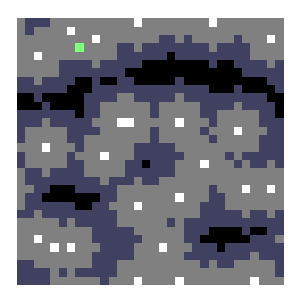
\includegraphics{00_000_grid.eps}
}
\caption["`Leeres Szenario"' ohne Hindernisse]{"`Leeres Szenario"' ohne Hindernisse}
\label{empty_grid:fig}
\end{figure}


\subsection{Szenario mit zuf�llig verteilten Hindernissen}\label{random_scenario_definition:sec}

F�r das Szenario mit zuf�llig verteilten Hindernissen sind zwei Parameter pr�gend. So bestimmt der erste Parameter (Hindernissanteil~\(\lambda_{h}\)) den Prozentsatz an Hindernissen an der Gesamtzahl der Felder des Torus und der zweite Parameter (Verkn�pfungsfaktor~\(\lambda_{p}\)) den Grad inwieweit die Hindernisse zusammenh�ngen.\\

Bei der Erstellung des Szenarios bestimmt \(\lambda_{p}\) die Wahrscheinlichkeit f�r jedes einzelne angrenzende freie Feld, dass beim Verteilen der Hindernisse nach dem Setzen eines Hindernisses dort sofort ein weiteres Hindernis gesetzt wird. \(\lambda_{p} = 0,0\) erg�be somit eine v�llig zuf�llig verteilte Menge an Hindernissen, w�hrend ein Wert von \(1,0\) eine oder mehrere stark zusammenh�ngende Strukturen schafft. Wird der Prozentsatz an Hindernissen \(\lambda_{h}\) auf \(0,0\) gesetzt, dann entspricht diesem dem oben erw�hnten leeren Szenario. Ein Wert von \(1,0\) w�rde eine v�llige Abdeckung des Torus bedeuten und w�re f�r einen Test somit unbrauchbar. Hier sollen nur geringe Werte bis \(0,4\) betrachtet werden, wobei sp�ter in Tests sich auf Werte bis \(0,2\) beschr�nkt wird, da bei gro�en Hindernissanteil die lokalen Entscheidungen einzelner Agenten zu wichtig werden, da das Zielobjekt sich eher  in einem kleinen Bereich aufh�lt.\\

In Abbildung~(\ref{random_grid_005:fig}), Abbildung~(\ref{random_grid_01:fig}), Abbildung~(\ref{random_grid_02:fig}) und Abbildung~(\ref{random_grid_04:fig}) werden Beispiele f�r zuf�llige Szenarien mit \(\lambda_{h} = 0,05\), \(0,1\), \(0,2\) bzw. \(0,4\) und \(\lambda_{p} = 0,01\), \(0,5\) bzw. \(0,99\) dargestellt.

\begin{figure}[htbp]
\centerline{	
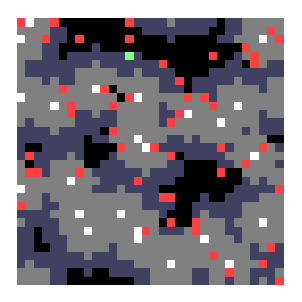
\includegraphics{005_001_grid.eps}
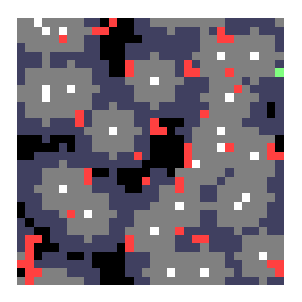
\includegraphics{005_050_grid.eps}
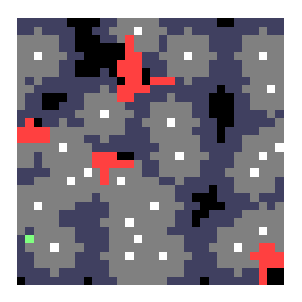
\includegraphics{005_099_grid.eps}
}
\caption[Szenario mit zuf�llig verteilten Hindernissen mit $\lambda_{h} = 0,05$] {Szenario mit zuf�llig verteilten Hindernissen mit Hindernissanteil \(\lambda_{h} = 0,05\) und Verkn�pfungsfaktor \(\lambda_{p} = 0,01\), \(0,5\) bzw. \(0,99\).}
\label{random_grid_005:fig}
\end{figure}

\begin{figure}[htbp]
\centerline{	
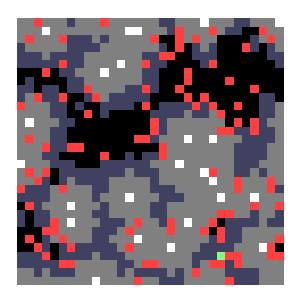
\includegraphics{01_001_grid.eps}
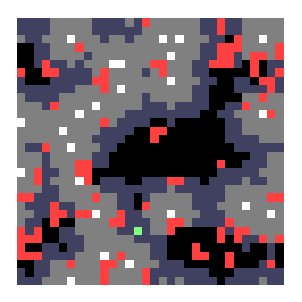
\includegraphics{01_050_grid.eps}
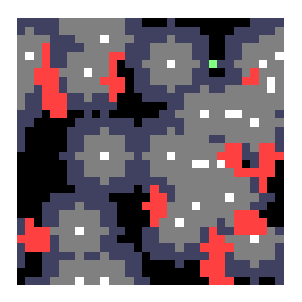
\includegraphics{01_099_grid.eps}
}
\caption[Szenario mit zuf�llig verteilten Hindernissen mit $\lambda_{h} = 0,1$] {Szenario mit zuf�llig verteilten Hindernissen mit Hindernissanteil \(\lambda_{h} = 0,1\) und Verkn�pfungsfaktor \(\lambda_{p} = 0,01\), \(0,5\) bzw. \(0,99\).}
\label{random_grid_01:fig}
\end{figure}

\begin{figure}[htbp]
\centerline{	
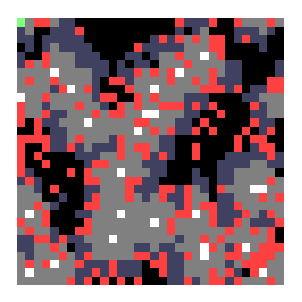
\includegraphics{02_001_grid.eps}
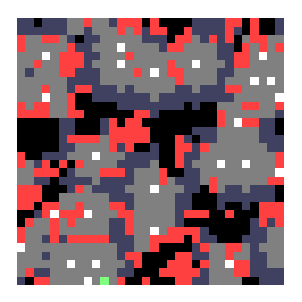
\includegraphics{02_050_grid.eps}
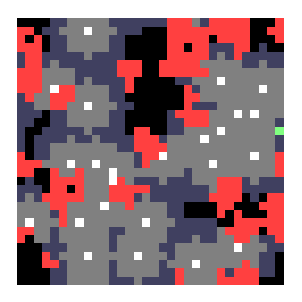
\includegraphics{02_099_grid.eps}
}
\caption[Szenario mit zuf�llig verteilten Hindernissen mit $\lambda_{h} = 0,2$] {Szenario mit zuf�llig verteilten Hindernissen mit Hindernissanteil \(\lambda_{h} = 0,2\) und Verkn�pfungsfaktor \(\lambda_{p} = 0,01\), \(0,5\) bzw. \(0,99\).}
\label{random_grid_02:fig}
\end{figure}

\begin{figure}[htbp]
\centerline{	
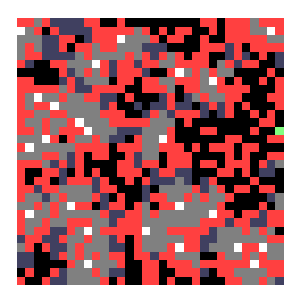
\includegraphics{04_001_grid.eps}
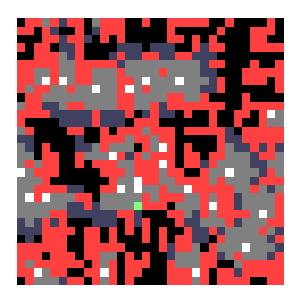
\includegraphics{04_050_grid.eps}
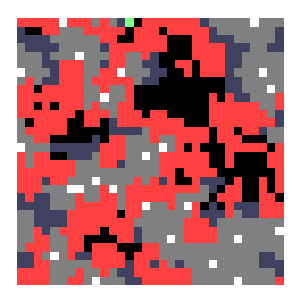
\includegraphics{04_099_grid.eps}
}
\caption[Szenario mit zuf�llig verteilten Hindernissen mit $\lambda_{h} = 0,4$] {Szenario mit zuf�llig verteilten Hindernissen mit Hindernissanteil \(\lambda_{h} = 0,4\) und Verkn�pfungsfaktor \(\lambda_{p} = 0,01\), \(0,5\) bzw. \(0,99\).}
\label{random_grid_04:fig}
\end{figure}


\subsection{S�ulenszenario}

In diesem Szenario werden regelm��ig, mit jeweils 7 Feldern Zwischenraum zueinander,  Hindernisse auf dem Torus verteilt. Tragende Idee dieses Szenarios ist es, dass die Agenten eine kleine Orientierungshilfe besitzen sollen, aber gleichzeitig m�glichst wenig Hindernisse verteilt werden. Das Zielobjekt startet an zuf�lliger Position, die Agenten starten mit m�glichst gro�em Abstand zum Zielobjekt.\\ Abbildung~\ref{pillar_grid:fig} zeigt ein Beispiel f�r den Startzustand eines solchen Szenarios, bei der das Zielobjekt sich in der Mitte und die Agenten am Rand befinden.

\begin{figure}[htbp]
\centerline{	
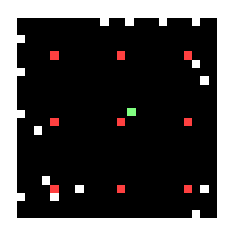
\includegraphics{pillar_grid.eps}
}
\caption[Startzustand des S�ulen Szenarios]{Startzustand des S�ulen Szenarios mit regelm��ig angeordneten Hindernissen und zuf�lliger Verteilung von Agenten mit m�glichst gro�em Abstand zum Zielobjekt}
\label{pillar_grid:fig}
\end{figure}



\subsection{Schwieriges Szenario}\label{difficult_scenario:sec}

Hier wird der Torus an der rechten Seite vollst�ndig durch Hindernisse blockiert, um den Torus zu halbieren. Alle Agenten starten (zuf�llig verteilt) am linken Rand, das Zielobjekt startet auf der rechten Seite.\\

In regelm��igen Abst�nden (7 Felder Zwischenraum) befindet sich eine vertikale Reihe von Hindernissen mit �ffnungen von 4 Feldern Breite abwechselnd im oberen Viertel und dem unteren Viertel.\\

Idee dieses Szenarios ist es, zu testen, inwieweit die Agenten durch die �ffnungen zum Ziel finden k�nnen. Ohne Orientierung an den �ffnungen und anderen Agenten ist es sehr schwierig, sich durch das Szenario zu bewegen. Die sp�ter besprochenen Tests in Kapitel~\ref{xcs_difficult_scenario:sec} werden zeigen, dass dieses Szenario besonders schwierig f�r sich zuf�llig bewegende Agenten und Agenten mit einfacher Heuristik ist und wie Kommunikation hier von Vorteil sein kann.\\
Abbildung~\ref{difficult_grid:fig} zeigt die Startkonfiguration des Szenarios.

\begin{figure}[htbp]
\centerline{	

\includegraphics{difficult_grid.eps}
}
\caption[Schwieriges Szenario]{Schwieriges Szenario mit fester, wallartiger Verteilung von Hindernissen in regelm��igen Abst�nden und mit �ffnungen, mit den Agenten mit zuf�lligem Startpunkt am linken Rand und mit dem Zielobjekt mit festem Startpunkt rechts oben}
\label{difficult_grid:fig}
\end{figure}

\section{Eigenschaften der Objekte}\label{sensoren:sec}

Jeder Agent bzw. das Zielobjekt besitzt eine Anzahl visueller, bin�rer Sensoren mit begrenzter Reichweite. Jeder Sensor kann nur feststellen, ob sich in seinem Sichtbereich ein Objekt eines bestimmten Typs befindet (\(1\)) oder nicht (\(0\)). Die Sensoren sind jeweils in eine bestimmte Richtung ausgerichtet, andere Objekte blockieren die Sicht und Sichtlinien werden durch einen einfachen Bresenham-Algorithmus~\cite{Bresenham} bestimmt.\\
Zwei Sensoren, die in dieselbe Richtung ausgerichtet sind und den selben Typ von Objekt erkennen, werden in diesem Zusammenhang ein Sensordatenpaar genannt (siehe Kapitel~\ref{sensor_datenpaar:sec}). Alle Sensoren, die nur gemeinsam haben, dass sie den selben Typ von Objekt erkennen, werden in einer Gruppe zusammengefasst und der Aufbau eines ganzen, aus solchen Gruppen bestehenden Sensordatensatzes soll in Kapitel~\ref{sensordatensatz:sec} besprochen werden. Die Eigenschaften der Agenten und des Zielobjekts selbst sollen dann in Kapitel~\ref{agents:cha} beschrieben werden.


\subsection{Sichtbarkeit von Objekten}\label{sichtbarkeit:sec}

Der Parameter \emph{sight range} bzw. \emph{reward range} bestimmt, bis zu welcher Distanz andere Objekte von einem Objekt als "`gesehen"' bzw. "`�berwacht"' gelten, sofern die Sicht durch andere Objekte nicht versperrt ist. Der Parameter \emph{reward range} ist relevant f�r die Bewertung der Qualit�t des Algorithmus (siehe Kapitel~\ref{qualitaet:sec}) und wird immer kleiner als der \emph{sight range} Wert gew�hlt. �ber die Sensoren kann ein Agent bzw. das Zielobjekt feststellen, ob sich Objekte in welcher der beiden Reichweiten befinden. Falls nicht anders angegeben sollen jeweils \emph{sight range} auf 5 und \emph{reward range} auf 2 gesetzt werden.\\


\subsection{Aufbau eines Sensordatenpaars}\label{sensor_datenpaar:sec}

Ein Datenpaar besteht aus zwei Sensoren, die den selben Typ von Objekt erkennen, in dieselbe Richtung ausgerichtet sind und sich nur in ihrer Sichtweite unterscheiden, wodurch der Agent rudiment�r die Entfernung zu anderen Objekten feststellen kann. Die Sichtweite des ersten Sensors eines Paares wird �ber den Parameter \emph{sight range} bestimmt, die Sichtweite des zweiten Sensors �ber den Parameter \emph{reward range} (siehe auch Kapitel~\ref{sichtbarkeit:sec}). Da \emph{sight range} \( > \) \emph{reward range} gilt, ist der �berwachte Bereich also eine Teilmenge des sichtbaren Bereichs. In Abbildung~\ref{sight_directions:fig} sind alle Sichtreichweiten (heller und dunkler Bereich) und �berwachungsreichweiten (heller Bereich) f�r die einzelnen Richtungen dargestellt.\\

\begin{figure}[htbp]
\centerline{	
\includegraphics{sight_directions.eps}
}
\caption[Sicht- und �berwachungsreichweite eines Agenten]{Sicht- ($5,0$, dunkler Bereich) und �berwachungsreichweite ($2,0$, heller Bereich) eines Agenten, jeweils f�r die einzelnen Richtungen}
\label{sight_directions:fig}
\end{figure}

Anzumerken sei hier, dass wegen der gew�hlten Werte f�r beide Reichweiten ein Sensordatenpaar (0\/1) nicht auftreten kann, da ein Objekt nicht gleichzeitig n�her als \(2,0\) und weiter als \(5,0\) entfernt sein kann.\\


\begin{figure}[H]
\setbox0\vbox{\small
Sei \(r(O1, O2)\) die Distanz zwischen dem Objekt, das die Sensordaten erfasst und dem n�chstliegenden Objekt des Typs, den der Sensor wahrnehmen kann, dann ergeben sich folgende F�lle:
\begin{enumerate}
\item (0/0) : \(r(O_1, O_2) > \) \emph{sight range} (kein passendes Objekt in Sichtweite)
\item (1/0) : \emph{reward range} \( < r(O_1, O_2) \le \) \emph{sight range} (Objekt in Sichtweite)
\item (1/1) : \(r(O_1, O_2) \le \) \emph{reward range} (Objekt in Sicht- und �berwachungsreichweite)
\item (0/1) : \emph{reward range} \(\ge r(O_1, O_2) > \) \emph{sight range} (Fall kann nicht auftreten, da \emph{reward range} \( < \) \emph{sight range})
\end{enumerate}
}
\centerline{\fbox{\box0}}
\end{figure}



\subsection{Aufbau eines Sensordatensatzes}\label{sensordatensatz:sec}

In einem Sensordatensatz sind jeweils 8 Sensoren zu jeweils einer Gruppe zusammengefasst, welche wiederum jeweils in 4 Richtungen mit jeweils einem Sensorenpaar aufgeteilt ist. Abbildung~\ref{sensordatensatz:fig} stellt den allgemeinen Aufbau eines kompletten Sensordatensatzes dar, der aus den drei Gruppen der Zielobjektsensoren (z), der Agentensensoren (a) und der Hinernisssensoren (h) besteht:\\


\begin{figure}[htbp]
\centerline{
$\mathrm{Sensordatensatz~} s = \underbrace{(z_{s_{N}} z_{r_{N}}) (z_{s_{O}} z_{r_{O}}) (z_{s_{S}} z_{r_{S}}) (z_{s_{W}} z_{r_{W}})}_{Erste~Gruppe~(Zielobjekt)}$
}
\centerline{
$\underbrace{(a_{s_{N}} a_{r_{N}}) (a_{s_{O}} a_{r_{O}}) (a_{s_{S}} a_{r_{S}}) (a_{s_{W}} a_{r_{W}})}_{Zweite~Gruppe~(Agenten)}$
$\underbrace{(h_{s_{N}} h_{r_{N}}) (h_{s_{O}} h_{r_{O}}) (h_{s_{S}} h_{r_{S}}) (h_{s_{W}} h_{r_{W}})}_{Dritte~Gruppe~(Hindernisse)}$
}
\caption[Darstellung des Sensordatensatzes] {Darstellung des Sensordatensatzes, eingeteilt in mehrere Gruppen und Sensorpaare}
\label{sensordatensatz:fig}
\end{figure}


Seien beispielsweise im Norden au�erhalb der �berwachungsreichweite aber in Sichtweite das Zielobjekt, im S�den ein oder mehrere Agenten in �berwachungsreichweite und im Westen und Osten sich ebenfalls in �berwachungsreichweite des Agenten befindliche Hindernisse, dann ergibt sich ein Sensordatensatz \(s_{Beispiel}\) wie in Abbildung~\ref{sensordatensatz_beispiel:fig} dargestellt.\\
 

\begin{figure}[htbp]
\centerline{	
$
s_{Beispiel} = (1, 0, 0, 0, 0, 0, 0, 0, 0, 0, 0, 0, 1, 0, 0, 0, 0, 0, 1, 1, 0, 0, 1, 1)
$
}
\caption[Beispiel f�r einen Sensordatensatz] {Beispiel f�r einen Sensordatensatz mit dem Zielobjekt im Norden, ein oder mehreren Agenten im S�den und Hindernissen im Westen und Osten}
\label{sensordatensatz_beispiel:fig}
\end{figure}


\subsection{Eigenschaften der Agenten und des Zielobjekts}\label{agents:cha}

Ein Agent kann in jedem Schritt zwischen vier verschiedenen Aktionen w�hlen, die den vier Richtungen (Norden, Osten, S�den, Westen) entsprechen. Dar�ber hinaus kann sich das Zielobjekt jedoch je nach Szenarioparameter auch mehrere Schritte bewegen, was in Kapitel~\ref{zielobjekt:sec} erl�utert wird.\\

Da ein Multiagentensystem auf einem diskreten Feld betrachtet werden soll, werden alle Agenten werden nacheinander in der Art abgearbeitet, dass jeder Agent die aktuellen Sensordaten (siehe Kapitel~\ref{sensoren:sec}) aus der Umgebung holt und auf deren Basis die n�chste Aktion bestimmt.\\
Wurden alle Aktionen bestimmt, k�nnen die Agenten in zuf�lliger Reihenfolge versuchen, sie auszuf�hren. Ung�ltige Aktionen, d.h. der Versuch sich auf ein besetztes Feld zu bewegen, schlagen fehl und der Agent f�hrt in diesem Schritt keine Aktion aus, wird aber auch nicht weiter bestraft. Eine detaillierte Beschreibung der Bewegung im Kontext anderer Agenten und Programmteile wird in Kapitel~\ref{reihenfolge:sec} gegeben.\\

Weitere F�higkeiten eines Agenten betreffen die Kommunikation, bis Kapitel~\ref{communication:cha} soll jedoch nur der Fall ohne Kommunikation betrachtet werden, d.h. die Agenten k�nnen untereinander keine Informationen austauschen und m�ssen sich alleine auf ihre Sensordaten verlassen.\\

Auf dem Torus bewegt sich neben den Agenten auch das Zielobjekt. Es kann, wie die Agenten auch, unterschiedlichen Bewegungsarten folgen, besitzt aber au�erdem noch eine bestimmte Geschwindigkeit (siehe Kapitel~\ref{zielobjekt:sec}). Neben der Gr��e des Torus und den Hindernissen tragen diese Eigenschaften des Zielobjekts wesentlich zur Schwierigkeit eines Szenarios bei, da dieser die Aufenthaltswahrscheinlichkeiten des Zielobjekts unter Einbeziehung des Zustands des letzten Zeitschritts bestimmt. Springt das Zielobjekt beispielsweise auf zuf�llige auf dem Torus (siehe Kapitel~\ref{goal_zufaelliger_sprung:sec}), dann existiert keine Verbindung zwischen den Positionen des Zielobjekts zweier aufeinanderfolgender Zeiteinheiten und Lernen wird sehr schwierig, was sp�ter in Kapitel~\ref{zielobjekt_analyse_zufall_sprung:sec} gezeigt wird. Prim�r soll diese Form der Bewegung auch nur zur allgemeinen, vorbereitenden Analyse dienen, w�hrend einfache Bewegungen, wie die zuf�llige Bewegung (Kapitel~\ref{random_neighbor:sec}) bzw. die Bewegung mit einfacher Richtungs�nderung (Kapitel~\ref{direction_change:sec}) die sp�ter tiefer untersuchten Bewegungsarten darstellen. Danach soll noch das sich intelligent verhaltende Zielobjekt besprochen werden, was ebenfalls ein zentraler Punkt der sp�teren Analyse (in Kapitel~\ref{zielagent_analyse_intelligent:sec}) sein soll. Am Ende sollen dann zwei Sonderf�lle erw�hnt werden, zum einen ein Zielobjekt, das nur in dieselbe Richtung l�uft (Kapitel~\ref{no_direction_change:sec}), welches in Kapitel~\ref{communication:cha} zur Untersuchung des schwierigen Szenarios benutzt werden soll.


\section{Grunds�tzliche Algorithmen der Agenten}\label{base_agent_types:sec}

Neben denjenigen Algorithmen, die auf XCS basieren und in Kapitel~\ref{lcs:cha} besprochen werden, sollen hier einige, auf einfachen Heuristiken basierende, Algorithmen vorgestellt werden, um die Qualit�t der anderen Algorithmen besser einordnen zu k�nnen. Wesentliches Merkmal im Vergleich zu auf XCS basierenden Algorithmen ist, dass sie statische, handgeschriebene Regeln benutzen und den Erfolg oder Misserfolg ihrer Aktionen ignorieren, d.h. ihre Regeln w�hrend eines Laufs nicht anpassen.\\
Die in Kapitel~\ref{implementierung_ablauf:sec} erw�hnte und dort aufgerufene Funktion \emph{calculateReward()} soll f�r die hier aufgelisteten Algorithmen also jeweils der leeren Funktion entsprechen. Im Folgenden sollen also insbesondere die Implementierungen der jeweiligen \emph{calculateNextMove()} Funktion vorgestellt werden.\\


\subsection{Algorithmus mit zuf�lliger Bewegung}\label{randomized_movement:sec}

Bei diesem Algorithmus wird in jedem Schritt wird eine zuf�llige Aktion ausgef�hrt. Abbildung~\ref{agent_random:fig} zeigt eine Beispielsituation, bei der der Agent jegliche Sensordaten (die 4 Agenten und das Zielobjekt, der als Stern dargestellt ist) ignoriert und eine Aktion zuf�llig ausw�hlen wird.\\
Programm~\ref{calculateNextMoveRandomAlgorithm:pro} zeigt den zugeh�rigen Quelltext.

\begin{figure}[htbp]
\centerline{	
\includegraphics{agent_random.eps}
}
\caption[Sich zuf�llig bewegender Agent]{Agent bewegt sich in eine zuf�llige Richtung (oder bleibt stehen).}
\label{agent_random:fig}
\end{figure}



\subsection{Algorithmus mit einfacher Heuristik}\label{simple_heuristik:sec}

Ist das Zielobjekt in Sichtweite, bewegt sich ein Agent mit dieser Heuristik  auf das Zielobjekt zu, ist es nicht in Sichtweite, f�hrt er eine zuf�llige Aktion aus. Abbildung~\ref{simple_agent_to_goal:fig} zeigt eine Beispielsituation bei der sich das Zielobjekt (Stern) im S�den befindet, der Agent mit einfacher Heuristik die anderen Agenten ignoriert und sich auf das Ziel zubewegen m�chte.\\
Programm~\ref{calculateNextMove_SimpleHeuristic:pro} zeigt den zugeh�rigen Quelltext.

\begin{figure}[htbp]
\centerline{	
\includegraphics{simple_agent_to_goal.eps}
}
\caption[Agent mit einfacher Heuristik]{Agent mit einfacher Heuristik: Sofern es sichtbar ist bewegt sich der Agent auf das Zielobjekt zu.}
\label{simple_agent_to_goal:fig}
\end{figure}



\subsection{Algorithmus mit intelligenter Heuristik}\label{intelligent_heuristik:sec}

Ist das Zielobjekt in Sicht, verh�lt sich diese Heuristik wie die einfache Heuristik. Ist das Zielobjekt dagegen nicht in Sicht, wird versucht, anderen Agenten auszuweichen, um ein m�glichst breit gestreutes Netz aus Agenten aufzubauen. In der Implementation hei�t das, dass unter allen Richtungen, in denen kein anderer Agent gesichtet wurde, eine Richtung zuf�llig ausgew�hlt wird und falls alle Richtungen belegt (oder alle frei) sind, wird aus allen Richtungen eine zuf�llig ausgew�hlt wird. In Abbildung~\ref{intelligent_agent:fig} ist das Zielobjekt nicht im Sichtbereich des Agenten und dieser w�hlt deswegen eine Richtung, in der die Sensoren keine Agenten anzeigen, in diesem Fall Norden.\\ Programm~\ref{calculateNextMove_IntelligentHeuristic:pro} zeigt den zugeh�rigen Quelltext.

\begin{figure}[htbp]
\centerline{	
\includegraphics{intelligent_agent.eps}
}
\caption[Agent mit intelligenter Heuristik]{Agent mit intelligenter Heuristik: Falls das Zielobjekt nicht sichtbar ist, bewegt sich der Agent von anderen Agenten weg.}
\label{intelligent_agent:fig}
\end{figure}



\section{Typen von Zielobjekten}\label{zielobjekt:sec}

Im Wesentlichen entspricht ein Zielobjekt einem Agenten, d.h. das Zielobjekt kann sich bewegen und besitzt Sensoren. Au�erdem kann sich das Zielobjekt in einem Schritt u.U. um mehr als ein Feld bewegen, was durch die durch das Szenario festgelegte Geschwindigkeit des Zielobjekts bestimmt ist. Der Wert der Geschwindigkeit kann auch gebrochene Werte annehmen, wobei in diesem Fall der gebrochene Rest dann die Wahrscheinlichkeit angibt, einen weiteren Schritt durchzuf�hren. Beispielsweise w�rde Geschwindigkeit \(1.4\) in \(40\%\) der F�lle zu zwei Schritten und in \(60\%\) der F�lle zu einem einzigen Schritt f�hren. Die Auswertung der Bewegungsgeschwindigkeit wird relevant in Kapitel~\ref{reihenfolge:sec}, bei der Reihenfolge der Ausf�hrung der Aktionen der Objekte.\\


Falls dem Algorithmus kein freies Feld zur Verf�gung steht, ist es allen Bewegungen des Zielobjektes gemeinsam, dass per Zufall ein freies Feld in der N�he ausgew�hlt und das Zielobjekt dorthin springt, was einem Neustart des Problems �hnlich ist. Dies ist notwendig, um eine Verf�lschung des Ergebnisses zu verhindern, welche eintreten kann, wenn einer oder mehrere Agenten (eventuell zusammen mit anderen Hindernissen) alle vier Bewegungsrichtungen des Zielobjekts dauerhaft zu blockieren. Zu beachten ist hier, dass auch der Sprung selbst eine Verf�lschung darstellt, insbesondere wenn in einem Durchlauf viele Spr�nge durchgef�hrt werden. Falls dies passiert sollte man deshalb das Ergebnis verwerfen und z.B. andere \emph{random seed} Werte oder einen anderen Algorithmus benutzen. Sofern nicht anders angegeben ist der Anteil solcher Spr�nge jeweils unter 0,1\% und wird ignoriert.\\


\subsection{Typ "`Zuf�lliger Sprung"'}\label{goal_zufaelliger_sprung:sec}

Ein Zielobjekt dieses Typs springt zu einem zuf�lligen Feld auf dem Torus. Ist das Feld besetzt, wird wiederholt, bis ein freies Feld gefunden wurde. Mit dieser Einstellung kann die Abdeckung des Algorithmus gepr�ft werden, d.h. inwieweit die Agenten jeweils au�erhalb der �berwachungsreichweite anderer Agenten bleiben.\\
Jegliche Anpassung an die Bewegung des Zielobjekts ist hier wenig hilfreich, ein Agent kann nicht einmal davon ausgehen, dass sich das Zielobjekt in der N�he seiner Position der letzten Zeiteinheit befindet.\\


\subsection{Typ "`Zuf�llige Bewegung"'}\label{random_neighbor:sec}

Ein Zielobjekt dieses Typs verh�lt sich so wie ein Agent mit dem Algorithmus mit zuf�lliger Bewegung (siehe Kapitel~\ref{randomized_movement:sec}). Sind alle m�glichen Felder belegt, wird, wie oben beschrieben, auf ein zuf�lliges Feld gesprungen.\\


\subsection{Typ "`Einfache Richtungs�nderung"'}\label{direction_change:sec}

Dieser Typ eines Zielobjekts entfernt zuerst alle Richtungen, in denen sich direkt angrenzend ein Hindernis befindet. Diese Erweiterung der F�higkeiten der Sensoren wurde gew�hlt, damit das Zielobjekt nicht in Hindernissen l�ngere Zeit steckenbleibt.\\
Anschlie�end wird die Richtung entfernt, die der im letzten Schritt gew�hlten entgegengesetzt ist. Von den verbleibenden (bis zu) drei Richtungen wird schlie�lich eine zuf�llig ausgew�hlt. Sind alle drei Richtungen versperrt, wird in die entgegengesetzte Richtung zur�ckgegangen.\\
In Abbildung~\ref{goal_agent_one_direction_change:fig} sind alle Felder grau markiert, die das Zielobjekt innerhalb von zwei Schritten erreichen kann, nachdem er sich einmal nach Norden bewegt hat.

\begin{figure}[htbp]
\centerline{	
\includegraphics{goal_direction_change.eps}
}
\caption[Zielobjekt mit maximal einer Richtungs�nderung]{Zielobjekt macht pro Schritt maximal eine Richtungs�nderung}
\label{goal_agent_one_direction_change:fig}
\end{figure}


\subsection{Typ "`Intelligentes Verhalten"'}\label{zielobjekt_intelligentes_verhalten:sec}

Hier versucht das Zielobjekt bei der Auswahl der Aktion m�glichst die Aktion zu w�hlen, bei der es au�erhalb der Sichtweite der Agenten bleibt. Dazu werden alle Richtungen gestrichen, in denen ein Agent sich innerhalb der �berwachungsreichweite befindet. Au�erdem werden von den verbleibenden Richtungen mit 50\% diejenigen Richtungen gestrichen, in denen sich ein Agent in Sichtweite befindet. Sind alle Richtungen gestrichen worden, bewegt sich das Zielobjekt zuf�llig. Sind alle Richtungen blockiert, springt es wie in den anderen Varianten auch auf ein zuf�lliges Feld in der N�he.\\

In Abbildung~\ref{goal_agent_intelligent:fig} wird die Richtung S�den gestrichen, da sich dort ein Agent in �berwachungsreichweite befindet. Die Richtungen Westen und Norden werden jeweils mit Wahrscheinlichkeit 50\% gestrichen, da sich dort Agenten in Sichtweite befinden. Nur Richtung Osten wird als M�glichkeit sicher �brig bleiben.\\

\begin{figure}[htbp]
\centerline{	
\includegraphics{goal_intelligent.eps}
}
\caption[Sich intelligent verhaltendes Zielobjekt weicht Agenten aus.]{Sich intelligent verhaltendes Zielobjekt weicht Agenten aus.}
\label{goal_agent_intelligent:fig}
\end{figure}


\subsection{Typ "`Beibehaltung der Richtung"'}\label{no_direction_change:sec}

Ein Zielobjekt dieses Typs versucht, immer Richtung Norden zu gehen. Ist das Zielfeld blockiert, w�hlt es ein zuf�lliges, angrenzendes, freies Feld im Westen oder Osten. Anzumerken ist, dass dies zus�tzliche F�higkeiten darstellen, d.h. das Zielobjekt kann feststellen, ob sich direkt angrenzend ein Hindernis im Norden befindet, w�hrend normale Agenten, was die Distanz betrifft, keine Informationen dar�ber besitzen k�nnen.\\

In Abbildung~\ref{goal_agent_always_same_direction:fig} sind drei Situationen dargestellt, zum einen ein wiederholtes Hin- und Herlaufen unter den Hindernissen, der Weg links um die Hindernisse herum und der Weg rechts um die Hindernisse herum.\\

Diese Art von Zielobjekt soll insbesondere im schwierigen Szenario benutzt werden um den Bereich, den das Zielobjekt �berquert, m�glichst gering zu halten, aber gleichzeitig das Zielobjekt auch nicht an einer Stelle stehen zu lassen.\\

\begin{figure}[htbp]
\centerline{	
\includegraphics{goal_always_same_direction.eps}
}
\caption[Bewegungsform "`Beibehaltung der Richtung"': Zielobjekt das sich, wenn m�glich, immer nach Norden bewegt]{Bewegungsform "`Beibehaltung der Richtung"': Zielobjekt bewegt sich, wenn m�glich, immer nach Norden.}
\label{goal_agent_always_same_direction:fig}
\end{figure}


\subsection{Typ "`Lernendes Zielobjekt"'}\label{zielobjekt_sxcs_einfuehrung:sec}

Ein besonderer Typ ist dieses Zielobjekt. Es kann mit Hilfe einer der in Kapitel~\ref{lcs_variants:cha} besprochenen Algorithmen lernen. Wesentlicher Unterschied zu lernenden Agenten ist, dass hier das Zielobjekt eine Aktion als positiv vermerkt, wenn sich keine Agenten in �berwachungsreichweite befinden. Eine genaue Beschreibung folgt in Kapitel~\ref{variant_zielobjekt_xcs_sxcs:sec}, hier soll die Idee nur der Vollst�ndigkeit halber erw�hnt werden.

\chapter{Das Zielobjekt}\label{zielobjekt:cha}

Auf dem Torus bewegt sich neben den Agenten auch das Zielobjekt. Es kann, wie die Agenten auch, unterschiedlichen Bewegungsarten folgen, besitzt aber au�erdem noch eine bestimmte Geschwindigkeit (Kapitel~\ref{base_properties_goal:sec}). Neben der Gr��e des Torus und den Hindernissen tragen diese Eigenschaften des Zielobjekts wesentlich zur Schwierigkeit eines Szenarios bei, da dieser die Aufenthaltswahrscheinlichkeiten des Zielobjekts unter Einbeziehung des Zustands des letzten Zeitschritts bestimmt. Springt das Zielobjekt beispielsweise auf zuf�llige auf dem Torus (siehe Kapitel~\ref{goal_zufaelliger_sprung:sec}), dann gibt es keine Verbindung zwischen den Positionen des Zielobjekts zweier aufeinanderfolgender Zeiteinheiten und Lernen wird sehr schwierig, was sp�ter in Kapitel~\ref{zielobjekt_analyse_zufall_sprung:sec} gezeigt wird. Prim�r soll diese Form der Bewegung auch nur zur allgemeinen, vorbereitenden Analyse dienen, w�hrend einfache Bewegungen, wie die zuf�llige Bewegung (Kapitel~\ref{random_neighbor:sec}) bzw. die Bewegung mit einfacher Richtungs�nderung (Kapitel~\ref{direction_change:sec}) die sp�ter tiefer untersuchten Bewegungsarten darstellen. Danach soll noch das sich intelligent verhaltende Zielobjekt besprochen werden, was ebenfalls ein zentraler Punkt der sp�teren Analyse (in Kapitel~\ref{zielagent_analyse_intelligent:sec}) sein soll. Am Ende sollen dann zwei Sonderf�lle erw�hnt werden, zum einen ein Zielobjekt, das nur in die selbe Richtung l�uft (Kapitel~\ref{no_direction_change:sec}), welches in Kapitel~\ref{communication:cha} zur Untersuchung des schwierigen Szenarios benutzt werden soll.


\section{Basiseigenschaften}\label{base_properties_goal:sec}

Im wesentlichen entspricht ein Zielobjekt einem Agenten, d.h. das Zielobjekt kann sich bewegen und besitzt Sensoren. Au�erdem kann sich das Zielobjekt in einem Schritt u.U. um mehr als ein Feld bewegen, was durch die durch das Szenario festgelegte Geschwindigkeit des Zielobjekts bestimmt ist. Der Wert der Geschwindigkeit kann auch gebrochene Werte annehmen, wobei in diesem Fall der gebrochene Rest dann die Wahrscheinlichkeit angibt, einen weiteren Schritt durchzuf�hren. Beispielsweise w�rde Geschwindigkeit \(1.4\) in \(40\%\) der F�lle zu zwei Schritten und in \(60\%\) der F�lle zu einem einzigen Schritt f�hren. Die Auswertung der Bewegungsgeschwindigkeit ist relevant in Kapitel~\ref{reihenfolge:sec}, bei der Reihenfolge der Ausf�hrung der Aktionen der Objekte.\\
Zus�tzlich dazu haben alle Arten von Bewegungen des Zielobjekts gemeinsam, dass, wenn dem Algorithmus kein freies Feld zur Verf�gung steht, ein zuf�lliges, freies Feld in der N�he ausgew�hlt und dorthin gesprungen wird. Dies kommt einem Neustart gleich und ist notwendig um eine Verf�lschung des Ergebnisses zu verhindern, das daher r�hren kann, dass ein oder mehrere Agenten (zusammen mit eventuellen Hindernissen) alle vier Bewegungsrichtungen des Zielobjekts blockieren.\\
Zu beachten ist hier, dass auch der Sprung selbst eine Verf�lschung darstellt, insbesondere wenn in einem Durchlauf viele Spr�nge durchgef�hrt werden. Falls dies passiert sollte man deshalb das Ergebnis verwerfen und z.B. andere \emph{random seed} Werte oder einen anderen Algorithmus benutzen. Sofern nicht anders angegeben ist der Anteil solcher Spr�nge jeweils unter 0.1\% und wird ignoriert.\\

TODO weiss schon dass blockiert


\section{Typen von Zielobjekten}

TODO EInleitung

\subsection{Typ "`Zuf�lliger Sprung"'}\label{goal_zufaelliger_sprung:sec}

Ein Zielobjekt dieses Typs springt zu einem zuf�lligen Feld auf dem Torus. Ist das Feld besetzt wird wiederholt bis ein freies Feld gefunden wurde. Mit dieser Einstellung kann die Abdeckung des Algorithmus gepr�ft werden, d.h. inwieweit die Agenten jeweils au�erhalb der �berwachungsreichweite anderer Agenten bleiben.\\
Jegliche Anpassung an die Bewegung des Zielobjekts ist hier wenig hilfreich, ein Agent kann nicht einmal davon ausgehen, dass sich das Zielobjekt in der N�he seiner Position der letzten Zeiteinheit befindet.\\


\subsection{Typ "`Zuf�llige Bewegung"'}\label{random_neighbor:sec}

Ein Zielobjekt dieses Typs verh�lt sich so wie ein Agent mit dem Algorithmus mit zuf�lliger Bewegung (siehe Kapitel~\ref{randomized_movement:sec}). Sind alle m�glichen Felder belegt, wird, wie oben beschrieben, auf ein zuf�lliges Feld gesprungen.\\


\subsection{Typ "`Einfache Richtungs�nderung"'}\label{direction_change:sec}

Ein Zielobjekt dieses Typs entfernt zuerst alle Richtungen, in denen sich direkt angrenzend ein Hindernis befindet. Diese Erweiterung der Sensorf�higkeiten wurde gew�hlt, damit das Zielobjekt nicht in Hindernissen l�ngere Zeit steckenbleibt.
Anschlie�end wird die Richtung entfernt, die der im letzten Schritt gew�hlten entgegengesetzt ist. Von den verbleibenden (bis zu) drei Richtungen wird schlie�lich eine zuf�llig ausgew�hlt. Sind alle drei Richtungen versperrt, wird in die entgegengesetzte Richtung zur�ckgegangen.\\
In Abbildung~\ref{goal_agent_one_direction_change:fig} sind alle Felder grau markiert, die der Zielagent innerhalb von zwei Schritten erreichen kann, nachdem er sich einmal nach Norden bewegt hat.

\begin{figure}[htbp]
\centerline{	
\includegraphics{goal_direction_change.eps}
}
\caption[Zielobjekt mit maximal einer Richtungs�nderung]{Zielobjekt macht pro Schritt maximal eine Richtungs�nderung}
\label{goal_agent_one_direction_change:fig}
\end{figure}


\subsection{Typ "`Intelligentes Verhalten"'}\label{zielobjekt_intelligentes_verhalten:sec}

Ein Zielobjekt dieses Typs versucht bei der Auswahl der Aktion m�glichst die Aktion zu w�hlen, bei der es au�erhalb der Sichtweite der Agenten bleibt. Dazu werden alle Richtungen gestrichen, in denen ein Agent sich innerhalb der �berwachungsreichweite befindet. Au�erdem werden von den verbleibenden Richtungen mit 50\% diejenigen Richtungen gestrichen, in denen sich ein Agent in Sichtweite befindet. Sind alle Richtungen gestrichen worden, bewegt sich das Zielobjekt zuf�llig. Sind alle Richtungen blockiert, springt es wie in den anderen Varianten auch auf ein zuf�lliges Feld in der N�he.\\

In Abbildung~\ref{goal_agent_intelligent:fig} wird die Richtung S�den gestrichen, da sich dort ein Agent in �berwachungsreichweite befindet. Die Richtungen Westen und Norden werden jeweils mit Wahrscheinlichkeit 50\% gestrichen, da sich dort Agenten in Sichtweite befinden. Nur Richtung Osten wird als M�glichkeit sicher �brigbleiben.

\begin{figure}[htbp]
\centerline{	
\includegraphics{goal_intelligent.eps}
}
\caption[Sich intelligent verhaltendes Zielobjekt der Agenten und Hindernissen ausweicht]{Zielobjekt bewegt sich mit bestimmter Wahrscheinlichkeit von Agenten und gr��erer Wahrscheinlichkeit von Hindernissen weg}
\label{goal_agent_intelligent:fig}
\end{figure}

\subsection{Typ "`Beibehaltung der Richtung"'}\label{no_direction_change:sec}

Der Zielobjekt versucht, immer Richtung Norden zu gehen. Ist das Zielfeld blockiert, w�hlt es ein zuf�lliges, angrenzendes, freies Feld im Westen oder Osten. Anzumerken ist, dass dies zus�tzliche F�higkeiten darstellen, d.h. das Zielobjekt kann feststellen, ob sich direkt angrenzend ein Hindernis im Norden befindet, w�hrend normale Agenten, was die Distanz betrifft, keine Informationen dar�ber besitzen k�nnen.\\ TODO

Sind auch die Felder im Westen und Osten belegt, springt es auf ein zuf�lliges freies Feld in der N�he. Schafft es der Zielobjekt innerhalb von einer bestimmten Zahl (Breite des Spielfelds) von Schritten nicht, einen weiteren Schritt nach Norden zu gehen, wird ebenfalls gesprungen, um ein "`festh�ngen"' an einem Hindernis zu vermeiden.\\

In Abbildung~\ref{goal_agent_always_same_direction:fig} sind drei Situationen dargestellt, zum einen ein wiederholtes hin- und herlaufen unter den Hindernissen, der Weg links um die Hindernisse herum und der Weg rechts um die Hindernisse herum.

\begin{figure}[htbp]
\centerline{	
\includegraphics{goal_always_same_direction.eps}
}
\caption[Bewegungsform "`Beibehaltung der Richtung"': Zielobjekt das sich, wenn m�glich, immer nach Norden bewegt]{Bewegungsform "`Beibehaltung der Richtung"': Zielobjekt bewegt sich, wenn m�glich, immer nach Norden}
\label{goal_agent_always_same_direction:fig}
\end{figure}

\subsection{Typ "`SXCS"'}\label{zielobjekt_sxcs_einfuehrung:sec}

Dieser Typ ist eine Implementierung f�r das Zielobjekt, das auf der SXCS Implementierung in Kapitel~\ref{lcs_variants:cha} basiert. Einziger Unterschied ist in der Art, wie das SXCS die eigenen Aktionen bewertet. W�hrend das dort beschriebene SXCS die N�he zum Zielobjekt belohnt, soll hier das Zielobjekt die Situationen positiv bewerten, bei denen sich keine Agenten in �berwachungsreichweite befinden. Eine genaue Beschreibung folgt im Kapitel~\ref{lcs_variants:cha}, hier sollte die Idee nur der Vollst�ndigkeit halber erw�hnt werden.

TODO Pendelbewegung?
TODO Fester Pfad?

\section{Bestimmung der Qualit�t eines Algorithmus}\label{qualitaet:sec}

Die Qualit�t eines Algorithmus zu einem Problem wird anhand des Anteils der Zeit berechnet, die er das Zielobjekt w�hrend des Problems �berwachen (d.h. das Zielobjekt innerhalb einer Distanz von h�chstens \emph{reward range} halten) konnte, relativ zur Gesamtzeit.\\
Die Qualit�t eines Algorithmus zu einer Anzahl von Problemen (also einem Experiment) wird Anhand des Gesamtanteil der Zeit berechnet, die er das Zielobjekt w�hrend aller Probleme �berwachen konnte, relativ zur Gesamtzeit aller Probleme.\\
Die Qualit�t eines Algorithmus entspricht dem Durchschnitt der Qualit�ten des Algorithmus mehrerer Experimente.\\
Die Halbzeitqualit�t eines Algorithmus zu einem Problem entspricht dem Anteil der Zeit, die der Algorithmus das Zielobjekt w�hrend jeweils der zweiten H�lfte des Problems �berwachen konnte, relativ zur halben Gesamtzeit.\\
Die Halbzeitqualit�t eines Algorithmus zu einer Anzahl von Problemen entspricht dem Anteil der Zeit, die der Algorithmus das Zielobjekt w�hrend jeweils der zweiten H�lfte des Problems �berwachen konnte, relativ zur halben Gesamtzeit aller Probleme.\\
Die Halbzeitqualit�t eines Algorithmus entspricht dem Durchschnitt aller Halbzeitqualit�ten des Algorithmus mehrerer Experimente.\\
Ein Vergleich der Qualit�t mit der Halbzeitqualit�t eines Algorithmus erm�glicht einen Einblick, wie gut sich der Algorithmus verh�lt, nachdem er sich auf das Problem bereits eine Zeit lang einstellen konnte.\\

\section{Ablauf der Simulation}\label{reihenfolge:sec}

Die Simulation selbst l�uft in ineinander geschachtelten Schleifen ab. Jede Konfiguration (in den abgedruckten Programmen jeweils �ber die globale Variable \emph{Configuration} angesprochen) wird �ber eine Reihe von Experimenten getestet (10 soweit nicht anders angegeben). F�r einen Test wird die Funktion \emph{doOneMultiStepExperiment()} (siehe Programm~\ref{mainExperiment:pro}) mit der aktuellen Nummer des Experiments als Parameter aufgerufen. In der Funktion wird ein neuer \emph{random seed} Wert initialisierung, der Torus auf den Startzustand gesetzt und schlie�lich das eigentliche Problem mit der Funktion \emph{doOneMultiStepProblem()} aufgerufen, welche in Programm~\ref{mainProblem:pro} abgebildet ist. Dort werden in einer Schleife alle Schritte durchlaufen und jeweils die Objekte abgearbeitet.\\

In welcher Reihenfolge dies geschieht, soll im Folgenden gekl�rt werden. Zusammenfassend ist zu sagen, dass zuerst die aktuelle Qualit�t und die aktuellen Sensordaten bestimmt werden. Daraus ermittelt jeder Agent die Bewertung f�r den letzten Schritt und bestimmt eine neue Aktion. Haben Agenten und das Zielobjekt diese Schritte abgeschlossen, werden ihre ermittelten Aktionen in zuf�lliger Reihenfolge ausgef�hrt.\\
TODO

Bei der Berechnung eines einzelnen Problems in der Funktion \emph{doOneMultiStepProblem()} stellt sich die Frage nach der Genauigkeit und der Reihenfolge der Abarbeitung, da die Simulation nicht parallel, sondern schrittweise auf einem diskreten Torus abl�uft. Dies kann u.U. dazu f�hren, dass je nach Position in der Liste abzuarbeitender Agenten die Informationen �ber die Umgebung unterschiedlich alt sind. Die Frage ist deshalb, in welcher Reihenfolge Sensordaten ermittelt, ausgewertet, Agenten bewegt, intern sich selbst bewertet und global die Qualit�t gemessen wird.\\

Da eine Aktion auf Basis der Sensordaten ausgew�hlt wird, ist die erste Restriktion, dass eine Aktion nach der Verarbeitung der Sensordaten stattfinden muss. Da au�erdem Aktionen bewertet werden sollen, also jeweils der Zustand nach der Bewegung mit dem gew�nschten Zustand verglichen werden soll, ist die zweite Restriktion, dass die Bewertung einer Aktion nach dessen Ausf�hrung stattfinden muss.\\

Unter diesen Voraussetzungen ergeben sich folgende zwei M�glichkeiten:

\begin{enumerate}
\item F�r alle Agenten werden erst einmal die neuen Sensordaten erfasst und sich f�r eine Aktion entschieden. Sind alle Agenten abgearbeitet, werden die Aktionen ausgef�hrt.
\item Die Agenten werden nacheinander abgearbeitet, es werden jeweils neue Sensordaten erfasst und sich sofort f�r eine neue Aktion entschieden. 
\end{enumerate}

Bei der ersten M�glichkeit haben alle Agenten die Sensordaten vom Beginn der Zeiteinheit, w�hrend bei der zweiten M�glichkeit sp�ter verarbeitete Agenten bereits die Aktionen der bereits berechneten Agenten miteinbeziehen k�nnen. Umgekehrt k�nnen dann fr�here Agenten bessere Positionen fr�her besetzen. Da aufgrund der primitiven Sensoren nicht davon auszugehen ist, dass Agenten beginnende Bewegungen (und somit deren jeweilige Zielposition) anderer Agenten einbeziehen k�nnen, soll jeder Agent von den Sensorinformationen zu Beginn der Zeiteinheit ausgehen.\\

Wenn sich mehrere Agenten auf dasselbe Feld bewegen wollen, dann spielt die Reihenfolge der Ausf�hrung der Aktionen eine Rolle. Wird die Liste der Agenten einfach linear abgearbeitet, k�nnen Agenten mit niedriger Position in der Liste die Aktion auf Basis j�ngerer Sensordaten f�llen. Dies kann dazu f�hren, dass Aktionen von Agenten mit h�herer Position in der Liste eher fehlschlagen, da das als frei angenommene Feld nun bereits besetzt ist. Da es keinen Grund gibt, Agenten mit niedrigerer Position zu bevorteilen, werden die Aktionen der Agenten in zuf�lliger Reihenfolge abgearbeitet.\\

Bez�glich der Bewegung ergibt sich hierbei eine weitere Frage, n�mlich wie unterschiedliche Bewegungsgeschwindigkeiten behandelt werden sollen, da alle Agenten eine Einheitsgeschwindigkeit von einem Feld pro Zeiteinheit haben, w�hrend sich das Zielobjekt je nach Szenario gleich eine ganze Anzahl von Feldern bewegen kann (siehe auch Kapitel~\ref{zielobjekt:sec}).\\

Die Entscheidung fiel hier auf eine zuf�llige Verteilung. Kann sich das Zielobjekt um \(n\) Schritte bewegen, so wird seine Bewegung in \(n\) Einzelschritte unterteilt, die nacheinander mit zuf�lligen Abst�nden (d.h. Bewegungen anderer Agenten) ausgef�hrt werden.\\

Eine weitere Frage ist, wie das Zielobjekt diese weiteren Schritte festlegen soll. Hier soll ein Sonderfall eingef�hrt werden, sodass das Zielobjekt in einer Zeiteinheit mehrmals (\(n\)-mal) neue Sensordaten erfassen und sich f�r eine neue Aktion entscheiden kann.



\subsection{Messung der Qualit�t}\label{qualitaetsmessung:sec}

Wie man die Qualit�t messen sollte, daf�r gibt es keinen Anhaltspunkt. Das zu verwendende Verfahren h�ngt davon ab, was man denn nun eigentlich erreichen m�chte, also auf welche Weise die Qualit�t des Algorithmus bewertet wird. Misst man die Qualit�t direkt nach der Bewegung des Zielobjekts, w�rde man diesem immer die M�glichkeit geben, sich noch vorher optimal zu positionieren, d.h. eine niedrigere Qualit�t w�re zu erwarten. Misst man sie immer zuvor, dann gilt das Umgekehrte f�r die Agenten.\\

Letztlich ist es eine Frage der Problemstellung, d.h. wann das Zielobjekt noch �berwacht gilt. Man denke z.B. an den Grenzfall, dass es sich gerade in die bzw. gerade aus der �berwachungsreichweite bewegt hat

Da ein wesentlicher Bestandteil die Kollaboration (und somit die Abdeckung des Torus anstatt dem Verfolgen des Zielobjekts) sein soll, soll ein Bewertungskriterium sein, inwieweit der Einfluss der Aktionen des Zielobjekts minimiert werden soll. D.h. die Agenten sollen sich m�glichst so verhalten, dass sie, unabh�ngig wie sich das Zielobjekt daraufhin bewegt, trotzdem m�glichst gut dastehen. Die Qualit�t wird somit nach der Bewegung des Zielobjekts gemessen. Die �berlegung unterstreicht auch nochmal, dass es besser ist, das Zielobjekt insgesamt wie einen normalen (aber sich mehrmals bewegenden) Agenten zu behandeln.\\

Spielt irgendwie keine Rolle... TODO raus!


\subsection{Reihenfolge der Ermittlung des \emph{base reward}}
TODO

Keine der bisher vorgestellten Varianten machen Gebrauch von einem sogenannten \emph{base reward}, d.h.  TODO

Schlie�lich bleibt die Frage danach, wann gepr�ft werden soll, ob das Zielobjekt in �berwachungsreichweite ist, und wann sich somit ein \emph{reward} ergeben soll. Wesentliche Punkte hierbei sind, dass der Algorithmus sich anhand der Sensordaten selbst bewertet und pro Zeitschritt die Sensordaten nur einmal erhoben werden. Letzteres folgt aus der Auslegung von XCS, der in der Standardimplementation darauf ausgelegt ist, dass der Reward jeweils genau einer Aktion zugeordnet ist. Daraus ergibt sich auch, dass der Reward von bin�rer Natur ist ("`Zielobjekt in �berwachungsreichweite"' oder "`Zielobjekt nicht in �berwachungsreichweite"'), weshalb Zwischenzust�nde f�r den Reward, der sich aus der mehrfachen Bewegung des Zielobjekts ergeben k�nnte, ausgeschlossen werden soll (z.B. "`War zwei von drei Schritten in der �berwachungsreichweite"' \(\Rightarrow \frac{2}{3}\) Reward). Insbesondere w�rde dies eine mehrfache Erhebung der Sensordaten erfordern.\\

TODO Rewarderhebung f�r normale Agenten irrelevant, evtl teilen und in XCS Kapitel

F�r den Reward ergeben sich somit folgende M�glichkeiten:

\begin{enumerate}
\item Ermittlung der einzelnen \emph{reward} Werte jeweils direkt nach der Ausf�hrung einer einzelnen Aktion
\item Ermittlung aller \emph{reward} Werte nach Ausf�hrung aller Aktionen der Agenten und des Zielobjekts
\end{enumerate}

Werden die \emph{reward} Werte sofort ermittelt (Punkt 1), dann bezieht sich der Wert auf die veralteten Sensordaten vor der Aktion, die Aktion selbst w�rde bei der Ermittlung des \emph{reward} Werts also ignoriert werden. Bei Punkt 2 m�sste man bis zum neuen Zeitschritt warten, bis neue Sensordaten ermittelt wurden.


\subsection{Zusammenfassung des Simulationsablaufs}

Zusammenfassend sieht der Ablauf aller Agenten (inklusive des Zielobjekts) also wie folgt aus:

\begin{figure}[H]
\setbox0\vbox{\small
\begin{enumerate}
\item Bestimmen der aktuellen \textbf{Qualit�t}
\item Erfassung aller \textbf{Sensordaten}
\item Bestimmung der jeweiligen {\bfseries {\em reward} Werte} f�r die einzelnen Objekte f�r den letzten Schritt
\item \textbf{Wahl der Aktion} anhand der Regeln des jeweiligen Agenten
\item \textbf{Ausf�hrung der Aktion} (in zuf�lliger Reihenfolge, das Zielobjekt wiederholt Schritte 1 und 2 nach der Ausf�hrung der Aktion)
\end{enumerate}
}
\centerline{\fbox{\box0}}
\end{figure}


\chapter{Erste Analyse der Agenten ohne LCS}

In diesem Kapitel sollen erste Analysen bez�glich der verwendeten Szenarien anhand des ``zuf�lligen Algorithmus''~\ref{randomized_movement:sec}, des Algorithmus mit ``einfacher Heuristik''~\ref{simple_heuristik:sec} und des Algorithmus mit ``intelligenter Heuristik''~\ref{intelligent_heuristik:sec} angefertigt werden. Die Ergebnisse aus der Analyse werden eine Grundlage f�r die vergleichende Betrachtung der Agenten mit LCS Algorithmen in Kapitel~\ref{lcs_analysis:cha} dienen, insbesondere werden sie Anhaltspunkte daf�r geben, welche Szenarien welche Eigenschaften der Algorithmen testen.

TODO: Ziel: Schwere Szenarien finden (schwierig f�r zuf�lligen, leicht f�r einfache heuristik)

\section{Statistische Merkmale}

Da keiner der hier vorgestellten Algorithmen lernt und somit statische Regeln besitzt, ist es nicht notwendig, die Qualit�ten der Algorithmen bei verschiedener Anzahl von Zeitschritten zu betrachten und zu vergleichen, die Zahl der Zeitschritte wird somit auf 500 festgesetzt. Au�erdem sollen in den Statistiken die Werte jeweils �ber einen Lauf von 10 Experimenten mit jeweils 10 Problemen ermittelt und gemittelt werden. Alle Werte sind auf 2 Stellen nach dem Komma gerundet. TODO

\subsection{Qualit�t}

\subsection{Abdeckung}

Die theoretisch maximal m�gliche Anzahl an Felder, die die Agenten innerhalb ihrer �berwachungsreichweite zu einem Zeitpunkt haben k�nnen, entspricht der Zahl der Agenten multipliziert mit der Zahl der Felder die ein Agent in seiner �bertragungsreichweite haben kann. Ist dieser Wert gr��er als die Gesamtzahl aller freien Felder, wird stattdessen dieser Wert benutzt.\\
Teilt man nun die Anzahl der momentan tats�chlich �berwachten Felder durch die eben ermittelte maximal m�gliche Anzahl an �berwachten Felder, erh�lt man die Abdeckung, die die Agenten momentan erreichen.\\

\subsection{Blockierte Bewegungen}

Der Wert der blockierten Bewegungen entspricht dem Anteil an Bewegungen, die insgesamt (Zielagent und Bewegungen gegen vom Zielagenten besetzte Felder ausgeschlossen) blockiert waren und somit nicht ausgef�hrt wurden. Der Wert ist ein 




\section{``Total Random'' Zielobjekt}

In allen Szenarien mit dieser Form der Bewegung des Zielobjekts kommt es nur darauf an, dass die Agenten einen m�glichst gro�en Bereich des Torus abdecken. 

\subsection{Ohne Hindernisse}

Ohne Hindernisse gibt sich ein klares Bild~(siehe~\ref{table:empty_total_random}), die intelligente Heuristik ist etwas besser als der des zuf�lligen Agenten und der einfachen Heuristik. Ein m�glichst weitr�umiges Verteilen auf dem Torus f�hrt zum Erfolg, was sich auch in einem hohen Wert der Abdeckung zeigt, denn genau das wird mit dem v�llig zuf�llig springenden Agenten getestet. Auch ist die Zahl der blockierten Bewegungen deutlich niedriger, was sich auch mit der Haltung des Abstands erkl�ren l�sst.\\
Die einfache Heuristik schneidet dagegen etwas schlechter als eine zuf�llige Bewegung ab. Zwar ist die Zahl der blockierten Bewegungen geringer, was sich dadurch erkl�ren l�sst, dass die einfache Heuristik zumindest an einem Punkt eine Sichtbarkeits�berpr�fung f�r die Richtung durchf�hrt, in der sie sich bewegen m�chte (n�mlich wenn das Zielobjekt in Sicht ist), andererseits ist die Abdeckung etwas geringer. Dies kommt daher, dass, wenn mehrere Agenten das Zielobjekt in der selben Richtung in Sichtweite haben, mehrere Agenten sich in die selbe Richtung bewegen. Dies beeintr�chtigt die zuf�llige Verteilung der Agenten auf dem Spielfeld und f�hrt somit auch zu einer niedrigeren Abdeckung des Torus.\\
Bez�glich der Anzahl der Agenten ergeben sich keine Besonderheiten, mit steigender Agentenzahl steigt die Zahl der blockierten Bewegungen (aufgrund gr��erer Anzahl von blockierten Feldern), w�hrend die Abdeckung sinkt (aufgrund sich �berlappender �berwachungsreichweiten).

\begin{table}[ht]
\caption{``Total Random'' ohne Hindernisse}
\centering
\begin{tabular}{c c c c c}
\hline\hline
Algorithmus & Agentenzahl & Blockierte Bewegungen & Abdeckung & Qualit�t \\ [0.5ex]
\hline
Zuf�llige Bewegung     & 8  & 2.84\% & 73.74\% & 32.43\% \\
Einfache Heuristik     & 8  & 2.81\% & 73.21\% & 32.12\% \\
Intelligente Heuristik & 8  & 0.63\% & 81.26\% & 36.01\% \\ [1ex]
\hline
Zuf�llige Bewegung     & 12 & 4.34\% & 69.49\% & 44.81\% \\
Einfache Heuristik     & 12 & 4.17\% & 68.89\% & 43.90\% \\
Intelligente Heuristik & 12 & 1.50\% & 77.57\% & 49.56\% \\ [1ex]
\hline
Zuf�llige Bewegung     & 16 & 5.81\% & 64.27\% & 54.57\% \\
Einfache Heuristik     & 16 & 5.67\% & 63.62\% & 54.05\% \\
Intelligente Heuristik & 16 & 2.85\% & 71.43\% & 60.73\% \\ [1ex]
\hline
\end{tabular}
\label{table:empty_total_random}
\end{table}

\subsection{S�ulenszenario}


\subsection{Zuf�llig verteilte Hindernisse}

Hier ergeben sich bei allen Einstellungen f�r \(\lambda_{h}\) und \(\lambda_{p}\) (siehe Kapitel~\ref{random_scenario_definition:sec}) ebenfalls ein klares Bild~(siehe~\ref{table:full_total_random}), die intelligente Heuristik liegt wieder vorne, gefolgt wieder von der einfachen Heuristik und der zuf�lligen Bewegung. Die einfache Heuristik schneidet minimal besser ab als die zuf�llige Bewegung, die Zahl der blockierten Bewegungen scheint hier st�rker ins Gewicht zu fallen. Insbesondere die intelligente Heuristik scheint Probleme mit den Hindernissen zu haben. Da Hindernisse in der Heuristik nicht beachtet werden, erzeugt die maximale Ausbreitung der Agenten einen Bewegungsdruck gegen sie.

\begin{table}[ht]
\caption{``Total Random'' mit Hindernisse (12 Agenten)}
\centering
\begin{tabular}{c c c c c c}
\hline\hline
Algorithmus & \(\lambda_{h}\) & \(\lambda_{p}\) & Blockierte Bewegungen & Abdeckung & Qualit�t \\ [0.5ex]
\hline
Zuf�llige Bewegung     & 0.2 & 0.99 & 14.25\% & 57.93\% & 46.89\% \\
Einfache Heuristik     & 0.2 & 0.99 & 11.96\% & 57.94\% & 46.99\% \\
Intelligente Heuristik & 0.2 & 0.99 & 17.76\% & 63.17\% & 51.39\% \\ [1ex]
\hline
Zuf�llige Bewegung     & 0.1 & 0.99 &  9.11\% & 64.04\% & 45.75\% \\
Einfache Heuristik     & 0.1 & 0.99 &  7.76\% & 63.82\% & 45.34\% \\
Intelligente Heuristik & 0.1 & 0.99 &  9.68\% & 70.50\% & 50.40\% \\ [1ex]
\hline
Zuf�llige Bewegung     & 0.1 & 0.5  & 11.89\% & 61.82\% & 44.62\% \\
Einfache Heuristik     & 0.1 & 0.5  & 10.27\% & 62.20\% & 44.32\% \\
Intelligente Heuristik & 0.1 & 0.5  & 12.21\% & 68.96\% & 49.16\% \\ [1ex]
\hline
\end{tabular}
\label{table:full_total_random}
\end{table}




Agenten. Der wesentliche zweite Faktor ist hier, dass der einfache Agent, wenn er das Zielobjekt in Sicht hat, davon ausgehen kann, dass sich in dieser Richtung wahrscheinlich kein Hindernis befindet, w�hrend der zuf�llige Agent Hindernisse �berhaupt nicht beachtet, somit �fters gegen ein Hindernis l�uft und letztlich �fters stehen bleibt. Der Unterschied zwischen beiden Agenten ist besonders hoch in Szenarien mit gr��erem Anteil an Hindernissen.\\

Ansonsten liegt der intelligente Agent wieder eindeutig vorne, beherrscht aber besonders gut Szenarien mit hohem ``Verkn�pfungsfaktor'' (\(1.0\)) der geringem Anteil an Hindernissen (\(0.1\)), bei denen er bis zu etwa 15\% �ber dem Ergebnis des einfachen Agenten liegt.\\
Dies liegt daran, dass Szenarien mit hohem ``Verkn�pfungsfaktors'' bedeuten, dass alle Hindernisse zusammenh�ngend einen gro�en Block bilden und somit dem Szenario ohne Hindernissen �hnlich sind, auf dem dieser Agent ja besonders gut abschneidet. In zerkl�ftete Szenarien hat der Algorithmus dagegen Schwierigkeiten um andere Agenten �berhaupt zu Gesicht bekommen, der Vorteil der Verteilung f�llt also zu einem Teil weg. 

Dies best�tigt auch ein Durchlauf bei dem Behinderungen der Sicht durch Hindernisse deaktiviert sind. Hierbei erreicht der intelligente Agent im Szenario (\(0.4\), \(0.1\)) statt TODO evtl weg

TODO

\section{``Zuf�lliger Nachbar'' und ``Einfache Richtungs�nderung''}

Wesentlicher Punkt bei beiden Bewegungstypen (siehe~\ref{random_neighbor:sec},~\ref{direction_change:sec}) ist, dass der jetzige Ort des Zielobjekts maximal zwei Felder (die Standardgeschwindigkeit des Zielobjekts in den Tests) vom Ort in der vorangegangenen Zeiteinheit entfernt ist. Somit ist ein lokales Einfangen eher von Relevanz, wenn auch das Zielobjekt grunds�tzlich schneller als andere Agenten ist.\\
Wesentlicher Unterschied zwischen beiden Bewegungstypen ist, dass das Zielobjekt mit Bewegungstyp ``zuf�lliger Nachbar'' bei einer Bewegungsgeschwindigkeit von 2 mit einer Wahrscheinlichkeit von \(\frac{1}{4}\) auf das urspr�ngliche Feld zur�ckkehrt, innerhalb eines Zeitschritts also stehenbleibt. Wie die Ergebnisse in Tabellen~\ref{table:neighbor_change_random} und ~\ref{table:neighbor_change_pillar} zeigen (TODO vielleicht noch n�her darauf eingehen), ergibt sich dadurch ein leichteres Szenario. Ein mitunter stehenbleibender Agent kann mittels Heuristiken leichter �berwacht werden, w�hrend es keine signifikante Ver�nderung bei der zuf�lligen Bewegung ergibt. In weiteren Tests soll deswegen immer nur die Bewegungsform ``Einfache Richtungs�nderung'' getestet werden.

%%TODO table:neighbor_change_no_obstacles

\begin{table}[ht]
\caption{Vergleich ``Zuf�lliger Nachbar'' und ``Einfache Richtungs�nderung'' (12 Agenten, ohne Hindernisse)}
\centering
\begin{tabular}{c c c c}
\hline\hline
Algorithmus & Blockierte Bewegungen & Abdeckung & Qualit�t \\ [1ex]
\hline
``Zuf�lliger Nachbar'' \\ [1ex]
\hline
Zuf�llige Bewegung     &  4.26\% & 69.41\% & 45.75\% \\
Einfache Heuristik     &  8.24\% & 61.77\% & 80.32\% \\
Intelligente Heuristik &  5.20\% & 70.09\% & 84.20\% \\ [1ex]
\hline
``Einfache Richtungs�nderung'' \\ [1ex]
\hline
Zuf�llige Bewegung     &  4.23\% & 69.63\% & 48.79\% \\
Einfache Heuristik     &  7.20\% & 62.71\% & 69.78\% \\
Intelligente Heuristik &  4.07\% & 71.24\% & 74.53\% \\ [1ex]
\hline
\end{tabular}
\label{table:neighbor_change_no_obstacles}
\end{table}

\begin{table}[ht]
\caption{Vergleich ``Zuf�lliger Nachbar'' und ``Einfache Richtungs�nderung'' (12 Agenten, zuf�lliges Szenario mit $\lambda_{h} = 0.2$, $\lambda_{p} = 0.99$)}
\centering
\begin{tabular}{c c c c}
\hline\hline
Algorithmus & Blockierte Bewegungen & Abdeckung & Qualit�t \\ [1ex]
\hline
``Zuf�lliger Nachbar'' \\ [1ex]
\hline
Zuf�llige Bewegung     & 14.56\% & 57.80\% & 47.32\% \\
Einfache Heuristik     & 18.29\% & 51.22\% & 85.92\% \\
Intelligente Heuristik & 22.33\% & 57.06\% & 88.31\% \\ [1ex]
\hline
``Einfache Richtungs�nderung'' \\ [1ex]
\hline
Zuf�llige Bewegung     & 14.60\% & 57.78\% & 47.92\% \\
Einfache Heuristik     & 17.11\% & 52.38\% & 78.39\% \\
Intelligente Heuristik & 21.54\% & 57.76\% & 82.31\% \\ [1ex]
\hline
\end{tabular}
\label{table:neighbor_change_random}
\end{table}

\begin{table}[ht]
\caption{Vergleich ``Zuf�lliger Nachbar'' und ``Einfache Richtungs�nderung'' (12 Agenten, S�ulenszenario)}
\centering
\begin{tabular}{c c c c}
\hline\hline
Algorithmus & Blockierte Bewegungen & Abdeckung & Qualit�t \\ [1ex]
\hline
``Zuf�lliger Nachbar'' \\ [1ex]
\hline
Zuf�llige Bewegung     &  5.94\% & 67.75\% & 43.37\% \\
Einfache Heuristik     & 10.41\% & 59.85\% & 85.61\% \\
Intelligente Heuristik &  7.82\% & 68.10\% & 88.98\% \\ [1ex]
\hline
``Einfache Richtungs�nderung'' \\ [1ex]
\hline
Zuf�llige Bewegung     &  6.02\% & 67.60\% & 45.83\% \\
Einfache Heuristik     &  9.54\% & 60.34\% & 76.05\% \\
Intelligente Heuristik &  6.90\% & 68.75\% & 81.28\% \\ [1ex]
\hline
\end{tabular}
\label{table:neighbor_change_pillar}
\end{table}


\section{``Intelligent Open'' und ``Intelligent Hide''}

\ref{table:intelligent_open_hide_no_obstacles}
\ref{table:intelligent_open_hide_random}
\ref{table:intelligent_open_hide_pillar}

TODO: Erl�uterung!

Zu beachten sei, dass im Fall von ``Intelligent Hide'' eine relativ gro�e Nummer an Spr�ngen des Zielobjekts (siehe Kapitel~\ref{base_properties_goal:sec}) stattgefunden hat, was die Ergebnisse etwas verzerrt, die Zahl h�lt sich aber noch in Grenzen (bis zu ca. 0.5\% im Fall der einfachen und intelligenten Heuristik im Fall mit vielen Hindernissen).

\begin{table}[ht]
\caption{Vergleich ``Intelligent Open'' und ``Intelligent Hide'' (8 Agenten, ohne Hindernisse)}
\centering
\begin{tabular}{c c c c}
\hline\hline
Algorithmus & Abdeckung & Qualit�t \\ [1ex]
\hline
``Intelligent Open'' \\ [1ex]
\hline
Zuf�llige Bewegung     & 74.15\% & 11.32\% \\
Einfache Heuristik     & 60.90\% & 82.86\% \\
Intelligente Heuristik & 69.62\% & 85.74\% \\ [1ex]
\hline
``Intelligent Hide'' \\ [1ex]
\hline
Zuf�llige Bewegung     & 74.13\% & 12.26\% \\
Einfache Heuristik     & 69.43\% & 55.31\% \\
Intelligente Heuristik & 74.87\% & 64.41\% \\ [1ex]
\hline
\end{tabular}
\label{table:intelligent_open_hide_no_obstacles}
\end{table}

\begin{table}[ht]
\caption{Vergleich ``Intelligent Open'' und ``Intelligent Hide'' (8 Agenten, zuf�lliges Szenario mit $\lambda_{h} = 0.2$, $\lambda_{p} = 0.99$)}
\centering
\begin{tabular}{c c c c}
\hline\hline
Algorithmus & Abdeckung & Qualit�t \\ [1ex]
\hline
``Intelligent Open'' \\ [1ex]
\hline
Zuf�llige Bewegung     & 62.54\% & 13.37\% \\
Einfache Heuristik     & 52.23\% & 84.33\% \\
Intelligente Heuristik & 56.92\% & 85.12\% \\ [1ex]
\hline
``Intelligent Hide'' \\ [1ex]
\hline
Zuf�llige Bewegung     & 62.52\% & 13.10\% \\
Einfache Heuristik     & 50.17\% & 90.32\% \\
Intelligente Heuristik & 56.94\% & 90.45\% \\ [1ex]
\hline
\end{tabular}
\label{table:intelligent_open_hide_random}
\end{table}

\begin{table}[ht]
\caption{Vergleich ``Intelligent (Open)'' und ``Intelligent (Hide)'' (8 Agenten, S�ulenszenario)}
\centering
\begin{tabular}{c c c}
\hline\hline
Algorithmus & Abdeckung & Qualit�t \\ [1ex]
\hline
``Intelligent (Open)'' \\ [1ex]
\hline
Zuf�llige Bewegung     & 72.55\% & 11.58\% \\
Einfache Heuristik     & 57.19\% & 85.58\% \\
Intelligente Heuristik & 64.26\% & 91.18\% \\ [1ex]
\hline
``Intelligent (Hide)'' \\ [1ex]
\hline
Zuf�llige Bewegung     & 72.56\% & 11.78\% \\
Einfache Heuristik     & 58.45\% & 80.98\% \\
Intelligente Heuristik & 65.65\% & 86.38\% \\ [1ex]
\hline
\end{tabular}
\label{table:intelligent_open_hide_pillar}
\end{table}


\section{Always Same Direction}

TODO

leeres Szenario

\section{LCS}

Wird weiter unten besprochen.





\section{Zusammenfassung}

Wie wir gesehen haben gibt es also Szenarien in denen Abdeckung kaum eine Rolle spielt und lokale Entscheidungen eine wesentliche Rolle spielen. Dies wird es erleichtern, geeignete Szenarien im Kapitel~\ref{communication:cha} ``Kommunikation'' zu finden.


\chapter{Parameter}\label{cha:parameter}

Die Einstellungen der XCS Parameter der durchgef�hrten Experimente entsprechen weitgehend den Vorschl�gen in~\cite{Butz} (``Commonly Used Parameter Settings''). Eine Auflistung findet sich in Tabelle~\ref{table:lcs_parameter}. Im Folgenden sollen Parameter besprochen werden, die entweder in der Empfehlung offen gelassen sind, also klar vom jeweiligen Szenario abh�ngen, und solche, bei denen von der Empfehlung abgewichen wurde.\\
Mitunter f�hren andere Parametereinstellungen auch zu wesentlich besseren Ergebnissen. Dies muss man aber vorsichtig bewerten, wenn die erreichte Qualit�t unter der des zuf�lligen Algorithmus liegt, da eine Auswirkung sein kann, dass der Algorithmus nicht besser lernt, sondern sich umgekehrt eher wie der zuf�llige Algorithmus verh�lt. Ein Vergleich mit der Qualit�t des zuf�lligen Algorithmus wird deswegen jeweils immer angegeben.\\
Anzumerken sei, dass alle Tests jeweils mit den in Tabelle~\ref{table:lcs_parameter} angegebenen Parameterwerten durchgef�hrt wurde und bei jedem Test jeweils nur der zu untersuchende Wert ver�ndert wurde. Um  synchronisierte und vergleichbare Daten zu haben, wurden die Tests deshalb in mehreren Etappen durchgef�hrt, die angegebenen Testergebnisse entsprechen jeweils den endg�ltigen Ergebnissen.

\section{Parameter \emph{max population N}}\label{sec:max_population_parameter}

Der Wert von \emph{max population} bezeichnet die maximalen Gr��e der \emph{classifier set} Liste. Ein gr��erer Wert verl�ngert die Laufzeit linear (siehe~\ref{empty_grid_time_maxpop:fig}), ein kleinerer Wert erh�ht die Konkurrenz zwischen den \emph{classifiers}. Gr��ere Werte erlauben eine bessere Anpassung, da weniger \emph{classifier} w�hrend eines Laufs gel�scht werden m�ssen und mehr Pl�tze zur Speicherung der Erfahrungen zur Verf�gung steht. Auf der anderen Seite werden mehr Schritte ben�tigt um die f�r die jeweiligen \emph{classifier} ausreichend Erfahrung zu sammeln (siehe~\ref{empty_grid_quality_maxpop:fig}).\\
F�r den Overhead (Benutzung des zuf�lligen Algorithmus ohne XCS) ergab sich eine mittlere Laufzeit von \(1.77\) Sekunden pro Experiment bei 500 Schritten (bzw. \(6.65\) Sekunden bei 2000 Schritten), was die anf�ngliche Stagnierung bis \(N = 32\) erkl�rt. Die Tests liefen auf einem T7500, 2.2 GHz in einem einzelnen Thread.\\
In den Tests wird \textbf{\(N = 128\)} gesetzt, was als ausreichender Kompromiss zwischen den erw�hnten Faktoren erscheint.

 und �ber 10 Probleme, gemittelt �ber 10 Experimente

~\ref{time_map_size_correlation:fig}

\begin{figure}[htbp]
\centerline{	
\includegraphics{time_map_size_correlation.eps}
}
\caption[Auswirkung der Torusgr��e auf die Laufzeit (leeres Szenario)] {Darstellung der Auswirkung der Torusgr��e auf die Laufzeit im leeren Szenario, zuf�lliger Bewegung des Zielobjekts, 8 sich zuf�llig bewegenden Agenten}
\label{time_map_size_correlation:fig}
\end{figure}


\begin{figure}[htbp]
\centerline{	
\includegraphics{empty_grid_time_maxpop.eps}
}
\caption[Auswirkung des Parameters \emph{max population N} auf Laufzeit (leeres Szenario)] {Darstellung der Auswirkung des Parameters \emph{max population N} auf die Laufzeit im leeren Szenario, zuf�lliger Bewegung des Zielobjekts, 8 Agenten mit LCS Algorithmus}
\label{empty_grid_time_maxpop:fig}
\end{figure}

\begin{figure}[htbp]
\centerline{	
\includegraphics{empty_grid_quality_maxpop.eps}
}
\caption[Auswirkung des Parameters \emph{max population N} auf Qualit�t (leeres Szenario)] {Darstellung der Auswirkung des Parameters \emph{max population N} auf die Qualit�t im leeren Szenario, zuf�lliger Bewegung des Zielobjekts, 8 Agenten mit LCS Algorithmus}
\label{empty_grid_quality_maxpop:fig}
\end{figure}

\section{Maximalwert \emph{reward}}\label{sec:maximalwert_rho}

Der Wert der bei der Bewertung als \emph{reward} vergeben wird hat lediglich �sthetische Auswirkungen und wurde auf \(1.0\) gesetzt. In der Standardimplementation von XCS (siehe~\ref{multistep_calc_reward:fig}) ist der maximale \emph{reward} �quivalent mit dem Maximalwert von \(\rho\), da das Problem bei jedem positiven \emph{reward} Wert neugestartet wird, also entweder der \emph{reward} Wert aus dem letzten Schritt also immer \(0\) ist oder \emph{maxPrediction} auf \(0\) gesetzt wurde, und \(\rho = \) \emph{reward} \(+~\gamma \) \emph{maxPrediction} gilt.\\

In den hier vorgestellten XCS Varianten wird dagegen der \emph{reward} Wert absteigend, zusammen mit dem \emph{maxPrediction} Wert, an fr�here \emph{actionSet} Listen verteilt, \(\rho\) kann also gr��er als \(1.0\) werden. In diesem Bereich ist noch Bedarf an theoretischer Forschung, in Tests haben sich Werte bis \(3.0\) ergeben, welche aber vom jeweiligen Szenario abh�ngen. Wird das Zielobjekt (z.B. wegen Hindernissen oder gro�en Torusdimensionen) eher selten gesehen, f�llt der Wert geringer aus.\\

\section{Parameter \emph{accuracy equality} $\epsilon_{0}$}
Der Parameter \(\epsilon_{0}\) gibt an, unter welchem Wert zwei \emph{accuracy} Werte als gleich gelten sollen. Dies ist insbesondere bei der \emph{subsummation} Funktion und der Berechnung des \emph{accuracy} Werts von Bedeutung. In der Literatur~\cite{Butz} wird als Regel genannt, dass der Wert auf etwa 1\% des Maximalwerts von \(\rho\) gesetzt werden soll, den der erwartete Reward annehmen kann. Aufgrund der �berlegungen in~\ref{sec:maximalwert_rho} wird \(\epsilon_{0}\) f�r die neuen XCS Varianten auf \(0.02\) gesetzt, w�hrend es f�r die Standardimplementation von XCS auf \(0.01\) gesetzt wird. Ein Testdurchlauf auf dem S�ulenszenario (siehe Abbildung~\ref{pillar_epsilon0:fig}) ergibt aber, dass der Parameter keine besondere Auswirkung hat, weshalb der Wert auf \(0.01\) belassen wird.

\begin{figure}[htbp]
\centerline{	
\includegraphics{pillar_epsilon0.eps}
}
\caption[Auswirkung des Parameters \emph{accuracy equality} $\epsilon_{0}$ auf die Qualit�t (S�ulenszenario)] {Auswirkung des Parameters  \emph{accuracy equality} $\epsilon_{0}$ auf die Qualit�t im S�ulenszenario, zuf�lliger Bewegung des Zielobjekts, 8 Agenten mit SXCS Algorithmus}
\label{pillar_epsilon0:fig}
\end{figure}

\section{Parameter \emph{reward prediction discount} $\gamma$}
TODO Abschnitt entfernen
Auch f�r den Wert \emph{reward prediction discount} \(\gamma\) hat sich ein etwas h�herer Wert als sinnvoll erwiesen, als standardm��ig benutzt wird. Laut~\cite{Butz} h�ngt der Wert auch vom verwendeten Szenario ab. Ein h�herer Wert f�r \(\gamma\) bedeutet, dass die H�he des Werts, der �ber \emph{maxPrediction} weitergegeben wird, mit zeitlichem Abstand zur urspr�nglichen Bewertung mit einem \emph{reward}, weniger schnell abf�llt, wodurch eine l�ngere Verkettung von \emph{reward} Werten m�glich ist. Umgekehrt f�hren zu hohe Werte f�r \(\gamma\) zu der positiven Bewertung von \emph{classifiers} die am Erfolg gar nicht beteiligt waren, was sich negativ auf die Qualit�t auswirken kann.

Tabelle~\ref{table:prediction_discount} zeigt einen Vergleich der Qualit�t mit dem Standardwert \(\gamma = 0.71\) und dem f�r die in dieser Arbeit verwendeten Testszenarien gew�hlten Wert \(\gamma = 0.95\).\\

TODO 0.71 lassen

TODOTabelle prediction discount

\section{Parameter Lernrate $\beta$}\label{sec:learnrate_parameter}

F�r die Lernrate \(\beta\) hat sich ein etwas niedrigerer als in der Literatur angegebener Wert (\(0.01\)) als erfolgreich erwiesen. Die Lernrate bestimmt, wie stark ein ermittelter \emph{reward} Wert den \emph{prediction}, \emph{prediction error}, \emph{fitness} und \emph{action set size} Wert pro Aktualisierung beeinflusst.TODO
Auch dieser Parameter ist szenariospezifisch, �ber die konkrete Begr�ndung kann nur spekuliert werden, die Schwierigkeit des Szenarios 
TODO

Vergleichende Tests (siehe Abbildung~\ref{pillar_learning_rate_quality:fig} mit niedrigerem bzw. h�herem Wert haben zu einer etwas schlechteren Qualit�t gef�hrt. TODO

\begin{figure}[htbp]
\centerline{	
\includegraphics{pillar_learning_rate_quality.eps}
}
\caption[Auswirkung des Parameters \emph{learning rate} $\beta$ auf Qualit�t (S�ulenszenario)] {Auswirkung des Parameters \emph{learning rate} $\beta$ auf die Qualit�t im S�ulenszenario, zuf�lliger Bewegung des Zielobjekts, 8 Agenten mit SXCS Algorithmus}
\label{pillar_learning_rate_quality:fig}
\end{figure}



\section{Parameter \emph{reward prediction init} $p_{i}$}\label{sec:prediction_init}

In der Literatur werden Werte nahe Null bzw. 1\% von \(\rho\) als Initialisierung f�r den \emph{reward prediction} Wert eines \emph{classifiers} angegeben. W�hlt man einen Wert, der n�her am Durchschnitt der \emph{reward prediction} Werte der \emph{classifier} liegt, die sich in den besten L�sungen am Ende eines Testdurchlaufs befinden, so ist zu erwarten, dass die Anzahl der ben�tigten Aktualisierungen des \emph{reward prediction} Werts geringer ausf�llt, das System also schneller konvergiert. Diese �berlegung wird best�tigt durch entsprechende Tests (siehe~\ref{pillar_lcs_prediction_init_quality:fig}).\\
Wir setzen somit f�r SXCS den Parameter auf \(p_{i} = 1.0\).\\
TODO Standardverfahren?

\begin{figure}[htbp]
\centerline{	
\includegraphics{pillar_lcs_prediction_init_quality.eps}
}
\caption[Auswirkung des Parameters \emph{reward prediction init} $p_{i}$ auf Qualit�t (S�ulenszenario)] {Darstellung Auswirkung des Parameters \emph{reward prediction init} $p_{i}$ auf die Qualit�t im S�ulenszenario, zuf�lliger Bewegung des Zielobjekts, 8 Agenten mit SXCS Algorithmus}
\label{pillar_lcs_prediction_init_quality:fig}
\end{figure}

\section{Zuf�llige Initialisierung}\label{sec:random_init}

Normalerweise werden XCS Systeme mit leeren \emph{classifier set} Listen initialisiert, als Option wird jedoch auch eine zuf�llige Initialisierung erw�hnt~(\cite{Butz2006}), bei der zu Beginn die \emph{classifier set} Liste mit mehreren \emph{classifiers} mit zuf�lligen \emph{action} Werten und \emph{condition} Vektoren gef�llt wird.\\
Tests haben gezeigt (siehe Tabelle~\ref{table:lcs_initialization}), dass dadurch minimal bessere Ergebnisse erzielt werden, allerdings nur in Szenarien mit ausreichender Schrittzahl (\(>100\)). Dies l�sst sich darauf zur�ckf�hren, dass  anf�nglich gef�llte \emph{classifier set} Listen die \emph{matchSet} Listen relativ gro� lassen werden, somit die Auswirkungen anf�nglichen Lernens geringer ausfallen und sich die Agenten eher wie sich zuf�llig bewegende Agenten verhalten. Da hier durchgef�hrten Tests �ber 500 bzw. 2000 Schritte laufen, sollen somit die \emph{classifier set} Listen mit zuf�llig generierten \emph{classifiers} gef�llt werden.

\begin{table}[ht]
\caption{Vergleichende Tests f�r den den Start mit und ohne zuf�llig gef�llten \emph{classifier set} Listen}
\centering
\begin{tabular}{c c c c c}
\hline
Algorithmus & Agentenzahl & Schrittzahl & Abdeckung & Qualit�t \\ [0.5ex]
\hline
Zuf�lliger Agent & 8 & 500 & 60.64\% & 61.54\% \\
Multistep & 8 & 500 & 60.64\% & 61.54\% \\
LCS & 8 & 500 & 60.64\% & 61.54\% \\
NewLCS & 8 & 500 & 60.64\% & 61.54\% \\
Zuf�lliges Szenario  & 8 & 500 & 60.64\% & 61.54\% \\
S�ulenszenario & 8 & 100 & 1.0\% & 1.0\% \\
LCS Ohne Drehung & 8 & 2000 & 1.0\% & 1.0\% \\ [0.5ex]

LCS Mit Drehung & 8 & 100 & 1.0\% & 1.0\% \\
LCS Mit Drehung & 8 & 500 & 1.0\% & 1.0\% \\
LCS Mit Drehung & 8 & 2000 & 1.0\% & 1.0\% \\ [0.5ex]

Zuf�lliger Agent & 12 & 500 & 76.03\% & 76.59\% \\
Einfacher Agent & 12 & 500 & 67.30\% & 96.86\% \\
Intelligenter Agent & 12 & 500 & 86.85\% & 95.08\% \\ [0.5ex]

LCS Ohne Drehung & 12 & 100 & 1.0\% & 1.0\% \\
LCS Ohne Drehung & 12 & 500 & 1.0\% & 1.0\% \\
LCS Ohne Drehung & 12 & 2000 & 1.0\% & 1.0\% \\ [0.5ex]

LCS Mit Drehung & 12 & 100 & 1.0\% & 1.0\% \\
LCS Mit Drehung & 12 & 500 & 1.0\% & 1.0\% \\
LCS Mit Drehung & 12 & 2000 & 1.0\% & 1.0\% \\ [0.5ex]

\hline
\end{tabular}
\label{table:lcs_initialization}
\end{table}


\section{�bersicht �ber alle Parameterwerte}
\begin{table}[ht]
\caption{Verwendete Parameter (soweit nicht anders angegeben) und Standardparameter, TODO englisch/deutsch}
\centering
\begin{tabular}{c c c}
\hline\hline
Parameter & Wert & Standardwert ~\cite{Butz}\\ [0.5ex]
\hline
Max population \(N\) & \textbf{128} (siehe~\ref{sec:max_population_parameter})\\
Max value \(\rho\) & \textbf{1.0} (siehe~\ref{sec:maximalwert_rho}) & [10000]\\
Fraction mean fitness \(\delta\) & 0.1 & [0.1]\\
Deletion threshold \(\theta_{\mathrm{del}}\) & 20.0 & [\(\sim\) 20.0]\\
Subsumption threshold \(\theta_{\mathrm{sub}}\) & 20.0 & [20.0+]\\
Covering \(\#\) probability \(P_{\#}\) & 0.5 & [\(\sim\) 0.33]\\
GAthreshold \(\theta_{\mathrm{GA}}\) & 25.0 & [25-50]\\
Mutation probability \(\mu\) & \(0.05\) & [0.01-0.05]\\
Prediction error reduction & 0.25 & [0.25]\\
Fitness reduction & \(0.1\) & [0.1]\\

Prediction init \(p_{i}\) & \textbf{0.5, 1.0} (siehe~\ref{sec:prediction_init}) & [\(\sim\) 0]\\
Prediction error init \(\epsilon_{i}\) & 0.0 & [0.0]\\
Fitness init \(F_{i}\) & \(0.01\) &  [0.01]\\
Random init & \textbf{ja} & [ja oder nein]\\
Numerosity & 1 & [1]\\
Experience & 0 & [0]\\

Accuracy equality \(\epsilon_{0}\) & \textbf{0.05} & [\emph{1\% des gr��ten Werts}]\\
Accuracy calculation \(\alpha\) & 0.1 & [0.1]\\
Accuracy power \(\nu\) & 5.0 & [5.0]\\
Prediction discount \(\gamma\) & 0.71 & [0.71]\\

Learning rate \(\beta\) & \textbf{0.01} (siehe~\ref{sec:learnrate_parameter}) & [0.1-0.2]\\

exploration probability & 0.5 (siehe~\ref{subsummation:sec}) & [\(\sim\) 0.5]\\ [0.5ex]

\hline
\end{tabular}
\label{table:lcs_parameter}
\end{table}





\chapter{XCS}\label{lcs:cha}

Jeder Agent besitzt ein unabh�ngiges, sogennantes \emph{eXtended Classifier System} (XCS), welches einem speziellen \emph{learning classifier system} (LCS) entspricht. Ein LCS ist ein evolution�res Lernsystem, das aus einer Reihe von \emph{classifier} Regeln besteht, die zusammen ein sogenanntes \emph{classifier set} bilden (siehe Kapitel~\ref{uebersicht_classifier:sec}). Eine allgemeine Einf�hrung in LCS findet sich z.B. in~\cite{Butz2006a}.\\

Das auf Genauigkeit der \emph{classifier} basierende XCS wurde zuerst in \cite{wilson:95} beschrieben und stellt eine wesentliche Erweiterung von LCS dar. Neben neuer Mechanismen zur Generierung neuer \emph{classifier} (insbesondere im Bereich bei der Anwendung des genetischen Operators) ist im Vergleich zum LCS gibt es vor allem innerhalb der Funktion zur Berechnung der \emph{fitness} Werte der \emph{classifier} Unterschiede. W�hrend der \emph{fitness} Wert beim einfachen LCS lediglich auf dem \emph{reward prediction error} Wert basierte, basiert bei XCS der \emph{fitness} Wert auf der Genauigkeit der jeweiligen Regel. Eine ausf�hrliche Beschreibung findet sich in~\cite{Butz2006}.\\

Im einfachsten Fall, im sogenannten \emph{single step} Verfahren erfolgt die Bewertung einzelner \emph{classifier}, also der Bestimmung eines jeweils neuen \emph{fitness} Werts, sofort nach Aufruf jeder einzelnen Regel, w�hrend im sogenannten \emph{multi step} Verfahren mehrere aufeinanderfolgende Regeln erst dann bewertet werden, sobald ein Ziel erreicht wurde.\\

TODO evtl teilweise in Scenario!
TODO zusammentun evtl mit Bewertung, s.u.

Ein klassisches Beispiel f�r den Test \emph{single step} Verfahren ist das 6-Multiplexer Problem~\cite{Butz2006}, bei dem das XCS einen Multiplexer simulieren soll, der bei der Eingabe von 2 Adressbits und 4 Datenbits das korrekte Datenbit liefert. Sind beispielsweise die 2 Adressbits auf "`10"' und die 4 Datenbits auf "`1101"', so soll das dritte Datenbit, also "`0"' zur�ckgeben. Im Gegensatz zum �berwachungsszenario kann also �ber die Qualit�t eines XCS direkt bei jedem Schritt entschieden werden. In Abbildung~\ref{6multiplexer:fig} findet sich eine schematische Darstellung des Problems.

\begin{figure}[htbp]
\centerline{	
\includegraphics{6multiplexer.eps}
}
\caption[Schematische Darstellung des 6-Multiplexer Problems] {Schematische Darstellung des Das 6-Multiplexer Problems}
\label{6multiplexer:fig}
\end{figure}

Ein klassisches Beispiel f�r \emph{multi step} Verfahren ist das \emph{Maze \(N\)} Problem, bei dem durch ein Labyrinth mit dem k�rzesten Weg von \(N\) Schritten gegangen werden muss. Am Ziel angekommen wird der zuletzt aktivierte \emph{classifier} positiv bewertet und das Problem neugestartet. Bei den Wiederholungen erh�lt jede Regel einen Teil der Bewertung des folgenden \emph{classifier}. Somit wird eine ganze Kette von \emph{classifier} bewertet und sich der optimalen Wahrscheinlichkeitsverteilung angen�hert, welche repr�sentiert, welche der Regeln in welchem Ma� am L�sungsweg beteiligt sind. 


Als Demonstration soll das in Abbildung~\ref{simple_scenario_multistep:fig} dargestellte (sehr einfache) Szenario dienen. Die zum Agenten zugeh�rigen \emph{classifer} sind in Abbildung~\ref{simple_scenario_multistep_classifier:fig} dargestellt, wobei die 4 angrenzenden Felder f�r jeden \emph{classifier} jeweils die Konfiguration der Kondition darstellt und der Pfeil die Aktion (f�r eine genauere Beschreibung eines \emph{classifier} siehe Kapitel~\emph{classifier:sec}). Im ersten Durchlauf werden alle \emph{classifier} in jedem Schritt zuf�llig gew�hlt, dann erh�lt \emph{classifier} e) eine positive Bewertung. Im zweiten Durchlauf erh�lt dann \emph{classifer} c) einen von \emph{classifier} e) weitergegebene positive Bewertung und \emph{classifier} e) auf Position 3 wird mit h�herer Wahrscheinlichkeit als \emph{classifier} f) gew�hlt. Das geht so lange weiter, bis sich f�r \emph{classifier} \(b, c, e, g\) ein ausreichend gro�er Wert eingestellt hat und keine wesentlichen Ver�nderungen mehr auftreten.

\begin{figure}[htbp]
\centerline{	
\includegraphics{simple_scenario_multistep.eps}
}
\caption[Einfaches Beispiel zum XCS \emph{multi step} Verfahren] {Einfaches Beispiel zum XCS \emph{multi step} Verfahren}
\label{simple_scenario_multistep:fig}
\end{figure}

\begin{figure}[htbp]
\centerline{	
\includegraphics{simple_scenario_multistep_classifier.eps}
}
\caption[Vereinfachte Darstellung eines \emph{classifier set} f�r das Beispiel zum XCS \emph{multi step} Verfahren] {Vereinfachte Darstellung eines \emph{classifier set} f�r das Beispiel zum XCS \emph{multi step} Verfahren}
\label{simple_scenario_multistep_classifier:fig}
\end{figure}


Eine n�here Beschreibung bez�glich der Implementierung von und dem Unterschied zwischen dem \emph{single step} und \emph{multi step} Verfahren findet sich in \cite{butz01algorithmic}.\\

Die in dieser Arbeit verwendete Implementierung entspricht im Wesentlichen der Standardimplementation des \emph{multi step} Verfahrens von~\cite{Butz_xcsclassifier} (mit der algorithmischen Beschreibung des Algorithmus in~\cite{butz01algorithmic}), eine 

Besonderheit stellt allerdings die Problemdefinition dar, da es kein Ziel zu erreichen gibt, sondern �ber die Zeit hinweg ein bestimmtes Verhalten erreicht werden soll (die �berwachung des Zielobjekts). Somit gibt es auch kein Neustart des Problems und keinen festen Start- oder Zielpunkt. Zus�tzlich, durch die Bewegung der anderen Agenten und des Zielobjekts, ver�ndert sich die Umwelt in jedem Schritt, ein Lernen durch Wiederholung gemachter Bewegungsabl�ufe ist deswegen deutlich schwieriger.\\


Die meisten Implementationen und Varianten von XCS besch�ftigen sich mit Szenarios, bei denen das Ziel in einer statischen Umgebung gefunden werden muss. H�ufiger Gegenstand der Untersuchung in der Literatur sind insbesondere relativ einfache Probleme 6-Multiplexer Problem und Maze1 (z.B. in~\cite{Butz2006} \cite{wilson:95} \cite{xcs2}), w�hrend XCS mit Problemen gr��erer Schrittzahl zwischen Start und Ziel Probleme hat \cite{barry02stability} \cite{Banzhaf}. Zwar gibt es Ans�tze um auch schwierigere Probleme besser in den Griff zu bekommen (z.B. Maze5, Maze6, Woods14 in~\cite{Butz2005}), indem ein Gradientenabstieg in XCS implementiert wurde. Ein konkreter Bezug zu einem dynamischen �berwachungsszenario konnte jedoch in keiner dieser Arbeiten gefunden werden.\\

Bez�glich Multiagentensystemen und XCS gibt es haupts�chlich Arbeiten, die auf zentraler Steuerung bzw. \emph{OCS} \cite{Takadama} basieren, also im Gegensatz zum Gegenstand dieser Arbeit auf eine �bergeordnete Organisationseinheit bzw. auf globale Regeln oder globalem Regeltausch zwischen den Agenten zur�ckgreifen.\\
Arbeiten bez�glich Multiagentensysteme in Verbindung mit LCS im Allgemeinen finden sich z.B. in \cite{Benouhiba}, wobei es auch dort zentrale Agenten gibt, mit deren Hilfe die Zusammenarbeit koordiniert werden soll, w�hrend in dieser Arbeit alle Agenten dieselbe Rolle spielen sollen.\\

Vielversprechend war der Titel der Arbeit~\cite{Lujan2008}, ``Generation of Rule-based Adaptive Strategies for a Collaborative Virtual Simulation Environment''. Leider wird in der Arbeit nicht diskutiert, auf was sich der kollaborative Anteil bezog, da nicht mehrere Agenten benutzt worden sind. Auch konnte dort jeder einzelne Schritt mittels einer \emph{reward} Funktion bewertet werden, da es globale Information gab. Dies vereinfacht ein solches Problem deutlich und macht einen Vergleich schwierig.\\

Eine weitere Arbeit in dieser Richtung~\cite{Hercog02socialsimulation} beschreibt das "`El Farol"' Bar Problem (EFBP), welches dort mit Hilfe eines Multiagenten XCS System erfolgreich gel�st wurde. Die Vergleichbarkeit ist hier auch eingeschr�nkt, da es sich bei dem EFBP um ein \emph{single step} Problem handelt.\\

TODO Comm!

Eine der dieser Arbeit (bez�glich Multiagentensysteme) am n�chsten kommende Problemstellung wurde in \cite{1102281} vorgestellt. Dort wurde die jeweilige Bewertung unter den (zwei) Agenten aufgeteilt, es fand also eine Kommunikation des \emph{reward} Werts statt. Wie das Ergebnis in Verbindung mit den Ergebnissen dieser Arbeit interpretiert werden kann, wird in Kapitel~\ref{communication:cha} diskutiert.\\

In \cite{Miyazaki} wurde gezeigt, dass bei der Weitergabe der Bewertung Gruppenbildung von entscheidender Wichtigkeit ist. Nach bestimmten Kriterien werden Agenten in Gruppen zusammengefasst und die Bewertung anstatt an alle, jeweils nur an die jeweiligen Gruppenmitgliedern weitergegeben.
Dies best�tigen auch Tests in Kapitel~\ref{communication:cha}, bei der sich Agenten mit �hnelnden (was das Verhalten gegen�ber anderen Agenten betrifft) \emph{classifier set} Listen in Gruppen zusammengefasst wurden und zum Teil bessere Ergebnisse erzielt werden konnten als ohne Kommunikation.


\cite{Barry03limitsin} TODO

TODO
In Kapitel~\ref{lcs_variants:cha} werden dann die Implementierungen der 
calculateReward, calculateNextMove beschrieben
TODO
Limits in Long Path Learning with XCS
Gamma!

\section{�bersicht}\label{uebersicht_classifier:sec}



Ein XCS ist ein regelbasiertes evolution�res Lernsystem, das im Wesentlichen aus folgenden Elementen besteht:

TODO ausfuehrlicher




\section{Ablauf eines XCS}\label{ablauf_lcs:sec}

\begin{enumerate}
\item Vervollst�ndigung der \emph{classifier} Liste (\emph{covering}, siehe Kapitel~\ref{covering:sec})
\item Auswahl auf die Sensordaten passender \emph{classifier} (\emph{match set} Liste, siehe Kapitel~\ref{matching:sec})
\item Bestimmung der Auswahlart der Aktion (\emph{explore/exploit}, siehe Kapitel~\ref{auswahlart:sec})
\item Auswahl der Aktion TODO
\item Erstellung des zur Aktion zugeh�rigen Liste von \emph{classifier} (\emph{action set} Liste, siehe Kapitel~\ref{actionSet:sec})

, so dass es in der Liste \emph{classifier} deren 

TODO
Bei der Auswahl einer Aktion werden alle \emph{classifier} mit \emph{condition} Vektoren gesucht, die auf die aktuellen Sensordaten passen. Diese bilden dann das \emph{matchSet}.
\item Im n�chsten Schritt wird ein \emph{classifier} aus diesem \emph{matchset} ausgew�hlt und dessen Aktion gespeichert.
\item Schlie�lich wird anhand des \emph{match set} und der gew�hlten Aktion das \emph{action set} gebildet.
\end{enumerate}

\subsection{Covering}\label{covering:sec}

TODO

\subsection{Variable \emph{lastMatchSet}}\label{matching:sec}

In der \emph{lastMatchSet} Variable werden jeweils alle \emph{classifier} gespeichert, die den letzten Sensordatenvektor erkannt haben. Sie entspricht dem \emph{predictionArray} in der originalen Implementierung von XCS in~\cite{Butz_xcsclassifier}, dort werden au�erdem Vorberechnungen zur Auswahl des n�chsten \emph{classifier} f�r die Bewegung durchgef�hrt und die Ergebnisse gespeichert.\\

\subsection{Variable \emph{actionSet}}\label{actionSet:sec}

Ein \emph{actionSet} ist jeweils einer Zeiteinheit zugeordnet. Dort werden jeweils alle \emph{classifier} gespeichert, die zu diesem Zeitpunkt denselben \emph{action} Wert besitzen wie der f�r die Bewegung bestimmte \emph{classifier}. In der Standardimplementation von XCS wird jeweils nur das letzte \emph{actionSet} gespeichert, w�hrend in SXCS eine ganze Reihe (bis zu \emph{maxStackSize} St�ck) gespeichert werden.





\begin{enumerate}

\item Einer Menge an Regeln, sogenannte \emph{classifier} (siehe Kapitel~\ref{classifier:sec}), die zusammen ein \emph{classifier set} bilden

\item Einem Mechanismus zur Auswahl einer Aktion aus dem \emph{classifier set} (siehe Kapitel~\ref{auswahlart:sec})

\item Einem Mechanismus zur Zusammenfassung aller \emph{classifier} aus dem \emph{classifier set} mit gleicher Aktion zu einer \emph{action set} Liste.

\item Einem Mechanismus zur Evolution der \emph{classifier} (mittels genetischer Operatoren, siehe Kapitel~\ref{genetische_operatoren:sec})

\item Eine Mechanismus zur Bewertung der \emph{classifier} (mittels \emph{reinforcement learning}, siehe Kapitel~\ref{bewertung:sec})

\end{enumerate}

W�hrend die ersten drei Punkte bei allen hier vorgestellten XCS Varianten identisch sind, gibt es wesentliche Unterschiede bei der Bewertung der \emph{classifier}. Diese werden gesondert in Kapitel~\ref{lcs_variants:cha} im Einzelnen besprochen. Im Folgenden sollen nun die ersten drei Punkte n�her betrachtet werden.\\

\section{Classifier}\label{classifier:sec}

Ein \emph{classifier} besteht aus einer Anzahl im folgenden diskutierten Variablen die anhand der in Kapitel~\ref{cha:parameter} aufgelisteten Werte initialisiert werden. Wesentliche Teile sind der \emph{condition} Vektor (Kapitel~\ref{condition_vector:sec}) und der \emph{action} Wert (Kapitel~\ref{action_wert:sec}), alle restlichen Variablen dienen zur Berechnung der Wahrscheinlichkeit mit der der \emph{classifier} ausgew�hlt und dessen \emph{action} Wert ausgef�hrt wird.\\


\subsection{Der \emph{condition} Vektor}\label{condition_vector:sec}

Der \emph{condition} Vektor gibt die Kondition an, in welcher Situation der zugeh�rige \emph{classifier} ausgew�hlt werden kann, d.h. welche Sensordaten von dem jeweiligen \emph{classifier} erkannt werden. Der Aufbau des Vektors (siehe Abbildung~\ref{gruppen_condition_vector:fig}) entspricht dem Vektor der �ber die Sensoren erstellt wird (siehe Kapitel~\ref{sensordatensatz:sec}).

\begin{figure}[htbp]
\centerline{	
$\underbrace{z_{s_{N}} z_{r_{N}} z_{s_{O}} z_{r_{O}} z_{s_{S}} z_{r_{S}} z_{s_{W}} z_{r_{W}}}_{Erste~Gruppe~(Zielobjekt)}
\underbrace{a_{s_{N}} a_{r_{N}} a_{s_{O}} a_{r_{O}} a_{s_{S}} a_{r_{S}} a_{s_{W}} a_{r_{W}}}_{Zweite~Gruppe~(Agenten)}
\underbrace{h_{s_{N}} h_{r_{N}} h_{s_{O}} h_{r_{O}} h_{s_{S}} h_{r_{S}} h_{s_{W}} h_{r_{W}}}_{Dritte~Gruppe~(Hindernisse)}$
}
\caption[Einteilung des \emph{condition} Vektors] {Einteilung des \emph{condition} Vektors in drei Gruppen}
\label{gruppen_condition_vector:fig}
\end{figure}


\subsection{Platzhalter im \emph{condition} Vektor}\label{platzhalter:sec}

Neben den zu den Sensordaten korrespondierenden Werten \(0\) und \(1\) soll es noch einen dritten Zustand, den Platzhalter "`\#"', geben, der anzeigen soll, dass beim Vergleich zwischen Kondition und Sensordaten diese Stelle ignoriert werden soll. Eine Stelle im \emph{condition} Vektor mit Platzhalter gilt also als �quivalent zur korrespondierenden Stelle in den Sensordaten, egal ob sie mit \(0\) oder \(1\) belegt ist. Ein Vektor, der ausschlie�lich aus Platzhaltern besteht, w�rde somit bei der Auswahl immer in Betracht gezogen werden, da er auf alle m�glichen Kombinationen der Sensordaten passt. Umgekehrt k�nnen dadurch bei der Auswahl der \emph{classifier} mehrere \emph{classifier} auf einen gegebenen Sensordatenvektor passen. Diese bilden dann die sogenannte \emph{match set} Liste, aus welchem dann wie in Kapitel~\ref{auswahlart:sec} beschrieben der eigentliche \emph{classifier} ausgew�hlt wird.\\


\subsection{Vergleich des \emph{condition} Vektors mit den Sensordaten}

Beim Vergleich der Sensordaten und Daten aus dem \emph{condition} Vektor werden immer jeweils zwei Paare verglichen. In Kapitel~\ref{sensoren:sec} wurde erw�hnt, dass der Fall \((0/1\)) in den Sensordaten nicht auftreten kann, weswegen (um die Aufgabe nicht unn�tig zu erschweren) ein Datenpaar \((0/1\)) im \emph{condition} Vektor �quivalent zum Datenpaar \((1/1\)) sein soll, es damit also eine gewisse Redundanz gibt. Daraus folgt, dass auch das Datenpaar \((0/\#)\) zu \((\#/\#)\) �quivalent ist.

Es ergeben sich also folgende F�lle:

\begin{enumerate}
\item Sensorenpaar \((0/0)\) wird erkannt von \((0/0)\), \((\#, 0)\), \((0, \#)\), \((\#, \#)\)
\item Sensorenpaar \((1/0)\) wird erkannt von \((1/0)\), \((\#, 0)\), \((1, \#)\), \((\#, \#)\)
\item Sensorenpaar \((1/1)\) wird erkannt von \((1/1)\), \((\#, 1)\), \((1, \#)\), \((\#, \#)\), \((0/1)\), \((0/\#)\)
\end{enumerate}

Beispielsweise w�rden folgende Sensordaten von den folgenden \emph{condition} Vektoren erkannt:
\begin{verbatim}
Sensordaten:
(Zielobjekt in Sicht im Norden, Agent im Sicht im S�den, 
Hindernisse im Westen und Osten)
10 00 00 00 . 00 00 11 00 . 00 11 00 11

Beispiele f�r erkennende condition Vektoren:
10 00 00 00 . ## ## ## ## . 00 ## ## ##
## ## ## ## . ## ## #1 00 . 00 11 ## ##
#0 ## ## ## . ## ## 01 ## . ## 11 ## 11
\end{verbatim}


\subsection{Der \emph{action} Wert}\label{action_wert:sec}

Wird ein \emph{classifier} ausgew�hlt, wird eine bestimmte Aktion ausgef�hrt, die durch den \emph{action} Wert determiniert ist. Im Rahmen dieser Arbeit entsprechen diese Aktionsm�glichkeiten den 4 Bewegungsrichtungen, die in Kapitel~\ref{agents:cha} besprochen wurden.\\


\subsection{Der \emph{fitness} Wert}

Der \emph{fitness} Wert soll die allgemeine Genauigkeit des \emph{classifier}
repr�sentieren und wird �ber die Zeit hinweg sukzessive an die beobachteten \emph{reward} Werte angepasst. Der Wertebereich verl�uft zwischen \(0.0\) und \(1.0\) (maximale Genauigkeit). Insbesondere eines der fr�hesten Werke zu XCS \cite{wilson:95} besch�ftigte sich mit diesem Aspekt der Genauigkeit.\\


\subsection{Der \emph{reward prediction} Wert}

Der \emph{reward prediction} Wert des \emph{classifier} stellt die H�he des \emph{reward} Werts dar, von dem der \emph{classifier} erwartet, dass er ihn bei der n�chsten Bewertung erhalten wird.\\


\subsection{Der \emph{reward prediction error} Wert}

Der \emph{reward prediction error} Wert soll die Genauigkeit des \emph{classifier} bzgl. des \emph{reward prediction} Werts (die durchschnittliche Differenz zwischen \emph{reward prediction} und \emph{reward}) repr�sentieren. U.a. auf Basis dieses Werts wird der \emph{fitness} Wert des \emph{classifier} angepasst.\\


\subsection{Der \emph{experience} Wert}

Der \emph{experience} Wert des \emph{classifier} repr�sentiert die Anzahl, wie oft ein \emph{classifier} aktualisiert wurde, also wieviel Erfahrung er sammeln konnte. Im Wesentlichen dient dieser Wert als Entscheidungshilfe, ob auf die anderen Werte des \emph{classifier} vertraut werden kann bzw. ob der \emph{classifier} als unerfahren gilt und somit z.B. bei L�schung und Subsummation gesondert behandelt werden muss.\\


\subsection{Der \emph{numerosity} Wert}

Durch Subsummation (siehe Kapitel~\ref{subsummation:sec} und Kapitel~\ref{genetische_operatoren:sec}) k�nnen \emph{classifier} eine Rolle als \emph{macro classifier} spielen, d.h. \emph{classifier} die andere \emph{classifier} in sich beinhalten. Der \emph{numerosity} Wert gibt an, wieviele andere, sogenannte \emph{micro classifier} sich in dem jeweiligen \emph{classifier} befinden.\\


\section{Subsummation von \emph{classifier}}\label{subsummation:sec}

Die Benutzung von den oben erw�hnten Platzhaltern (Kapitel~\ref{platzhalter:sec}) erlaubt es dem XCS mehrere \emph{classifier} zu zusammenzulegen, wodurch die Gesamtzahl der \emph{classifier} sinkt und somit Erfahrungen, die ein XCS Agent sammelt, nicht unbedingt mehrfach gemacht werden m�ssen. Die dahinter stehende Annahme ist, dass es Situationen gibt, in denen der Gewinn der durch Unterscheidung zwischen zwei verschiedenen Sensordatens�tzen geringer ist als die Ersparnis durch das Zusammenlegen beider \emph{classifier}, d.h. dem Ignorieren der Unterschiede.\\

Besitzt ein \emph{classifier} sowohl einen gen�gend gro�en \emph{experience} Wert als auch einen ausreichend kleinen \emph{reward prediction error} Wert, so kann er als sogenannter \emph{subsumer} auftreten. Andere \emph{classifier} (in derselben \emph{action set} Liste, also mit gleichem \emph{action} Wert) werden durch den \emph{subsumer} ersetzt, sofern der von ihnen abgedeckte Sensordatenbereich eine Teilmenge des von dem \emph{subsumer} abgedeckten Bereichs ist, der \emph{subsumer} also an allen Stellen des \emph{condition} Vektors entweder denselben Wert wie der zu subsummierende \emph{classifier} oder einen Platzhalter besitzt.\\


\section{Genetische Operatoren}\label{genetische_operatoren:sec}

Es werden aus der jeweiligen \emph{action set} Liste zwei \emph{classifier} (die Eltern) zuf�llig ausgew�hlt und zwei neue \emph{classifier} (die Kinder) aus ihnen gebildet und in die Population eingef�gt. Dabei wird mittels \emph{two-point crossover} ein neuer \emph{condition} Vektor generiert und der \emph{action} Wert auf den der Eltern gesetzt (da sie aus derselben \emph{action set} Liste stammen, ist der Wert beider Eltern identisch). Die restlichen Werte werden standardm��ig wie in Kapitel~\ref{cha:parameter} aufgelistet initialisiert. Werden Kinder in die Population eingef�gt, deren \emph{action} Wert und \emph{condition} Vektor identisch mit existierenden \emph{classifier} ist, werden sie stattdessen subsummiert.\\
Da die Sensoren und somit auch der \emph{condition} Vektor aus drei in sich geschlossenen Gruppen bestehen, werden im Unterschied zur Standardimplementation beim \emph{crossing over} zwei feste Stellen benutzt, die die Gruppe f�r das Zielobjekt, die Gruppe f�r Agenten und die Gruppe f�r feste Hindernisse voneinander trennen.\\

Bezeichne \((z_1, a_1, h_1)\) bzw. \((z_2, a_2, h_2)\) jeweils die drei Gruppen (siehe Kapitel~\ref{condition_vector:sec}) des \emph{condition} Vektors des ersten bzw. zweiten ausgew�hlten Elternteils, dann k�nnen f�r die drei Gruppen der \emph{condition} Vektoren \((z_{1k}, a_{1k}, h_{1k})\) und \((z_{2k}, a_{2k}, h_{2k})\) der beiden Kinder folgende Kombinationen auftreten:

\[[(z_{1k}, a_{1k}, h_{1k}), (z_{2k}, a_{2k}, h_{2k})] = [(z_1, a_1, h_1) , (z_2, a_2, h_2)]\]
\[[(z_{1k}, a_{1k}, h_{1k}), (z_{2k}, a_{2k}, h_{2k})] = [(z_2, a_1, h_1) , (z_1, a_2, h_2)]\]
\[[(z_{1k}, a_{1k}, h_{1k}), (z_{2k}, a_{2k}, h_{2k})] = [(z_1, a_2, h_1) , (z_2, a_1, h_2)]\]
\[[(z_{1k}, a_{1k}, h_{1k}), (z_{2k}, a_{2k}, h_{2k})] = [(z_2, a_2, h_1) , (z_1, a_1, h_2)]\]






\section{Bewertung der Aktionen (\emph{base reward})}\label{bewertung:sec}

XCS ist darauf ausgelegt, dass es eine komplette, genaue und m�glichst allgemeine Darstellung einer \emph{reward} Funktion darstellt. Bei einer Problemstellung, die mit dem \emph{single step} Verfahren gel�st werden kann, entspricht die optimale Darstellung der \emph{reward} Funktion durch das XCS gleichzeitig auch der L�sung des eigentlichen Problems. Beispielsweise beim oben erw�hnten 6-Multiplexer Problem pr�ft die \emph{reward} Funktion, ob das XCS aus den 4 Datenbits anhand der 2 Steuerbits das richtige Datenbit gew�hlt hat, also ob das XCS so wie ein 6-Multiplexer funktioniert. Wesentliche Voraussetzung f�r das \emph{single step} Verfahren ist, dass der Agent globale Information besitzt, also in einem Schritt m�glichst alle Informationen zur L�sung des Problems zur Verf�gung hat, um die jeweilige L�sung zu bewerten.\\

Bei komplexeren Problemen, bei denen ein Agent nur lokale Informationen zur Verf�gung hat (beispielsweise bei \emph{Maze~\(N\)} die angrenzenden Felder), liefert die \emph{reward} Funktion nur eine Teilinformation, beispielsweise "`1"' beim letzten Schritt auf das Ziel und "`0"' sonst. Diese Art von Bewertung, die der Agent direkt aus den Sensordaten berechnet, soll in diesem Zusammenhang im folgenden \emph{base reward} genannt werden.\\

Die optimale Darstellung der \emph{reward} Funktion, die XCS zum \emph{base reward} in dem Beispiel liefern w�rde, w�re bis auf den letzten Schritt nicht besser als ein sich zuf�llig bewegender Agent, weshalb bei XCS der ermittelte \emph{base reward} auch an andere, am Gesamtweg beteiligte, \emph{action set} Listen in der Art weitergibt, dass Aktionen, die an einem k�rzeren Weg beteiligt sind, h�her bewertet werden.\\

Die in der Standardimplementation von XCS verwendete Weitergabe bezieht sich, wie in der Einf�hrung zu diesem Kapitel erl�utert wurde, auf schrittweise Weitergabe der Bewertungen an das vergangene \emph{action set}. 

TODO
Ergebnis: bringt nichts Agenten miteinzubeziehen, da nicht sichergestellt ist, dass der andere Agent den Agenten in Sicht hat mmh... Naja

Die Erweiterung beim �berwachungszenario im Vergleich zu TODO!

, wird die gemessene Qualit�t des Algorithmus davon abh�ngen, 
lokaler Reward!!!

Die Bewertung von Aktionen bzw. deren zugeh�rigen \emph{classifier} erfolgt in zwei Schritten. Zuerst soll anhand einer Heuristik (der \emph{reward} Funktion) bestimmt werden, ob die momentane Situation "`gut"' oder "`schlecht"' ist. Dies stellt den in dieser Arbeit genannten \emph{base reward} dar. Da 


Die Heuristik sollte so gestaltet sein, dass sie 

Foundations of Learning Classifier Systems By Larry Bull, Tim Kovacs
Evolutionary pressures in XCS



TODO Quelle?


Wie diese Heuristik, die im Allgemeinen genannte \emph{reward} Funktion, gestaltet wird, davon h�ngt sehr stark die Qualit�t des Systems ab. 



W�rde man beispielsweise nur die Position von Hindernissen 

Der \emph{base reward} 


Getestet wurde

goal in sight range
goal in reward range

goal in sight range, kein agent in reward range (selbe Richtung)
goal in sight range, kein agent in sight range (selbe Richtung)

BESTES von oben + kein Agent in Sicht


base reward

Programm~\ref{agent_check_reward:pro}

\newlisting{Bestimmung des \emph{base reward} Werts f�r Agenten}{agent_check_reward:pro}
/**
 * @return true Falls das Zielobjekt von diesem Agenten �berwacht wird
 *   und kein anderer Agent in dieser Richtung in 
 *   �berwachungsreichweite steht
 */
  public boolean checkRewardPoints() {
    boolean[] sensor_agent = lastState.getSensorAgent();
    boolean[] sensor_goal = lastState.getSensorGoal();
 
    for(int i = 0; i < Action.MAX_DIRECTIONS; i++) {
      if((sensor_goal[2*i]) && (!sensor_agent[2*i+1])) {
        return true;
      }
    }
    
    return false;
  }
\end{lstlisting}

TODO raus

\section{Auswahlart der \emph{classifier}}\label{auswahlart:sec}

In jedem Zeitschritt gilt es zu entscheiden, welche Bewegung ein Agent ausf�hren soll. Als Basis der Entscheidung hat ein Agent zum einen die Sensordaten und zum anderen das eigene \emph{classifier set} zur Verf�gung. Da ein Sensordatensatz von mehreren \emph{classifier} erkannt werden kann und in jedem Schritt somit mehrere passende \emph{classifier} samt Aktionen ausgew�hlt werden k�nnen (siehe Kapitel~\ref{platzhalter:sec}), stellt sich die Frage, welche der Aktionen ausgef�hrt werden soll.\\

In XCS wird dazu die zur jeweiligen Sensordatensatz passenden \emph{match set} Liste in vier (Anzahl der m�glichen Aktionen) Gruppen entsprechend des \emph{action} Werts des jeweiligen \emph{classifier} aufgeteilt um dann alle Produkte aus den \emph{fitness} und \emph{reward prediction} Werten der \emph{classifier} aus der jeweiligen Gruppe aufaddiert und durch die Summe der \emph{fitness} Werte der \emph{classifier} der jeweiligen Gruppe geteilt. Dieser Wert soll im folgenden \emph{predictionFitnessProductSum} genannt werden.\\

In der urspr�nglichen Implementierung \cite{Butz_xcsclassifier} wurden dann folgende Arten beschrieben, wie eine Aktion aus diesen vier ausgew�hlt werden kann:

\begin{enumerate}
\item \emph{random selection} : Zuf�llige Auswahl einer Aktion (identisch mit zuf�lliger Bewegung)
\item \emph{roulette wheel selection} : Zuf�llige Auswahl einer Aktion, Wahrscheinlichkeit abh�ngig vom \emph{predictionFitnessProductSum} Wert der jeweiligen Gruppe
\item \emph{best selection} : Auswahl der Aktion mit dem h�chsten \emph{predictionFitnessProductSum} Wert der jeweiligen Gruppe
\end{enumerate}

Im Folgenden sollen diese Auswahlarten n�her vorgestellt und au�erdem noch eine weitere Auswahlart aus der Literatur besprochen werden. Im n�chsten Abschnitt (Kapitel~\ref{exploreexploit:sec}) soll dann der Wechsel zwischen diesen Auswahlarten n�her untersucht und die tats�chlichen Testergebnisse (Kapitel~\ref{test_auswahlarten:sec}) zwischen den vorgestellten Varianten pr�sentiert werden.



\subsection{Auswahlart \emph{random selection}}

Bei einem dynamischen �berwachungsszenario ist es im Vergleich zu standardm��igen statischen Szenarien weder n�tig noch hilfreich \emph{random selection} zu nutzen. Die Idee f�r diese Auswahlart in einem statischen Szenario ist, dass man m�chte, dass das XCS m�glichst vielen verschiedenen Situationen ausgesetzt ist. Da in einem statischen Szenario Start- und Zielposition wie auch die Hindernisse fest sind, ist es wichtig, durch \emph{random selection} dem XCS einen gewissen Spielraum zu geben.\\

Bei einem dynamischen Szenario (siehe Kapitel~\ref{dynamisch_kollaborativ:sec}) ergibt sich dieses Problem nicht, andere Agenten und das Zielobjekt sind in stetiger Bewegung, der eigene Startpunkt ist nicht fixiert und das Problem wird bei Erreichen des Ziels nicht neugestartet. Aufgrund der Natur der Aufgabenstellung ist es in einem �berwachungsszenario au�erdem wichtig, dass das XCS �ber eine l�ngere Zeit hinweg eine gute Leistung liefert, also stetig gute Entscheidungen trifft, eine zuf�llige Auswahl scheint also wenig zielf�hrend zu sein.\\


\subsection{Auswahlart \emph{best selection}}\label{best_selection_auswahlart:sec}

Bei der Auswahlart~\emph{best selection} wird einfach nur die Aktion mit dem h�chsten \emph{predictionFitnessProductSum} Wert ausgew�hlt. Die Verwendung dieser Auswahlart kann u.U. schnell in eine Sackgasse bzw. zu langen Folgen gleicher Aktionen (beispielsweise andauernd gegen eine Wand laufen) f�hren, sofern sich die Umwelt nicht �ndert. Auf den ersten Blick scheint es zwar, dass z.B. zur Verfolgung von einem Zielobjekt ein kompromissloses Verhalten sinnvoll ist, jedoch bedarf dies zum einen bereits guter, gelernter \emph{classifier} und zum anderen vollst�ndige Information. In dem in dieser Arbeit betrachteten Szenario sind die Sensordaten allerdings beschr�nkt, der Agent wei� nicht genau, wo sich das Zielobjekt befindet, selbst wenn es in Sicht ist. Eine optimale Verhaltensstrategie muss hier also Entscheidungen auf Basis von Wahrscheinlichkeitsverteilungen treffen, weshalb die alleinige Verwendung der Auswahlart \emph{best selection} eher nicht in Frage kommt.\\


\subsection{Auswahlart \emph{roulette wheel selection}}

Bei dieser Auswahlart bestimmt der \emph{predictionFitnessProductSum} Wert (relativ zu den anderen \emph{predictionFitnessProductSum} Werten) die Wahrscheinlichkeit, ausgew�hlt zu werden. Diese Auswahlart erscheint sinnvoll, allerdings ist speziell bei diesem Szenario davon auszugehen, dass, wie auch schon in Kapitel~\ref{best_selection_auswahlart:sec} erw�hnt, es aufgrund mangelnder Sensorinformation keine eindeutig besten Aktionen gibt, weshalb sich die \emph{reward prediction} Werte der \emph{classifier} sich eher �hneln. Eine auf Proportionen ausgelegte Auswahlart wie \emph{roulette wheel selection} kann deshalb dazu f�hren, dass es kaum Unterschiede in den Auswahlwahrscheinlichkeiten gibt, mit der eine Aktion ausgew�hlt wird. Diese Auswahlart �hnelt somit eher der Auswahlart \emph{random selection} als \emph{best selection}.


\subsection{Auswahlart \emph{tournament selection}}\label{tournament_selection:sec}

Zu den oben erw�hnten drei M�glichkeiten wurde in \cite{Butz2003} eine weitere vorgestellt und in Bezug auf XCS diskutiert, die sogenannte \emph{tournament selection}. Als Vorteile werden geringerer Selektionsdruck, h�here Effizienz, geringerer Einfluss von St�rungen, wie auch Flexibilit�t der Anpassung �ber zwei Parameter, \(k\) und \(p\), genannt.\\
Bei dieser Auswahlart werden allgemein gesagt \(k\) Elemente aus einer Menge zuf�llig ausgew�hlt, nach ihrem zugeh�rigen Wert sortiert und absteigend mit Wahrscheinlichkeit \(p\) das jeweilige Element gew�hlt (d.h. das erste mit \(p\), das zweite mit \((1,0-p)p\), das dritte mit \((1,0-p)^{2}p\) usw.).\\

In dem hier besprochenen Fall w�ren die Mengen immer der Gr��e 4 (Anzahl der Aktionen) und die Elemente entsprechen jeweils den berechneten \emph{predictionFitnessProductSum} Werten. Der Einfachheit soll \(k\) auf den Maximalwert gesetzt werden, damit alle Aktionen zumindest eine geringe Wahrscheinlichkeit besitzen, ausgew�hlt zu werden.\\

Im Grunde entspricht diese Auswahlart also der \emph{roulette wheel selection}, allerdings ohne dem Problem, dass die Auswahlwahrscheinlichkeit aufgrund �hnlicher Produkte sich ebenfalls �hneln. Diese Form der Auswahl, bei geeigneter Wahl von \(k\) und \(p\), scheint also am vielversprechend zu sein. Au�erdem ist die Darstellung selbst sehr flexibel, beispielsweise w�re \emph{tournament selection} mit \(p = 1,0\) und \(k = 4\) identisch mit \emph{best selection} und mit \(p = 1,0\) und \(k = 1\) w�re es identisch mit \emph{random selection}.\\ 

Bei der Implementierung dieser Auswahlart muss man aufpassen, dass bei der Sortierung Eintr�ge mit gleichem Produkt aus \emph{fitness} und \emph{reward prediction} in zuf�lliger Reihenfolge aufgef�hrt werden. Insbesondere am Anfang kann es sonst dazu kommen, dass alle Agenten in die selbe Richtung laufen.\\

Ein idealer Wert f�r \(p\) ergibt sich aus Abbildung~\ref{test_tournament_selectionp:fig} und Abbildung~\ref{test_tournament_selectionp2:fig}. Dort zur besseren �bersicht jeweils die Differenz zum Agenten mit zuf�lliger Bewegung dargestellt. Beide Testreihen liefen auf dem S�ulenszenario mit einem Zielobjekt mit Geschwindigkeit 1 bzw. 2, 2000 Schritten, mit Zielobjekt mit einfacher Richtungs�nderung bzw. mit einem sich intelligent verhaltendem Zielobjekt. Die Werte im Bereich von etwa \(0,75\) bis \(0,9\) erreichen sehr �hnliche Werte, da \(0,84\) etwa in der Mitte liegt und in vielen F�llen das beste Ergebnis erzielte, soll dieser Wert f�r die Tests gen�gen. Die beste Aktion wird also mit \(p = 84\%\) Wahrscheinlichkeit, die zweitbeste mit ca. \((1,0-p)p \approx 13\%\) Wahrscheinlichkeit, die drittbeste mit ca. \((1,0-p)^{2}p \approx 2\%\) Wahrscheinlichkeit und die schlechteste Aktion mit ca. \((1,0-p)^{3}p \approx 1\%\) Wahrscheinlichkeit gew�hlt.\\
Au�erdem kann man erkennen, dass bei einem sich intelligent verhaltenden Zielobjekt eine andauernde \emph{exploit} Phase die beste Wahl ist. Dies wird in Kapitel~\ref{test_auswahlarten:sec} relevant.\\


\begin{figure}[htbp]
\centerline{	
\includegraphics{test_tournament_selectionp.eps}
}
\caption[Vergleich verschiedener Werte $p$ f�r Auswahlart \emph{tournament selection} (Zielobjekt mit einfacher Richtungs�nderung)]{Vergleich verschiedener Werte $p$ f�r Auswahlart \emph{tournament selection} (Zielobjekt mit einfacher Richtungs�nderung, S�ulenszenario, 2000 Schritte)}
\label{test_tournament_selectionp:fig}
\end{figure}

\begin{figure}[htbp]
\centerline{	
\includegraphics{test_tournament_selectionp2.eps}
}
\caption[Vergleich verschiedener Werte $p$ f�r Auswahlart \emph{tournament selection} (intelligentes Zielobjekt)]{Vergleich verschiedener Werte $p$ f�r Auswahlart \emph{tournament selection} (intelligentes Zielobjekt, S�ulenszenario, 2000 Schritte)}
\label{test_tournament_selectionp2:fig}
\end{figure}



\subsection{Wechsel zwischen den \emph{explore} und \emph{exploit} Phasen}\label{exploreexploit:sec}

In der Standardimplementierung von XCS wird zwischen verschiedenen Auswahlarten hin und her geschalten. Die Auswahlarten werden in zwei Gruppen geteilt, in die sogenannte \emph{explore} Phase und in die \emph{exploit} Phase. In der \emph{exploit} Phase soll bevorzugt eine Auswahlart ausgef�hrt werden, die das Produkt aus den Werten \emph{fitness} und \emph{reward prediction} m�glichst stark gewichtet, \emph{best selection} und \emph{tournament selection} sind Kandidaten f�r die \emph{exploit} Phase, w�hrend \emph{random selection} und \emph{roulette wheel selection} Kandidaten f�r die \emph{explore} Phase w�ren. Idee ist, dass man mit Hilfe der \emph{explore} Phasen den Suchraum besser erforschen kann, dann aber zur eigentlichen Probleml�sung in der \emph{exploit} Phase m�glichst direkt auf das Ziel zugeht um \emph{classifier} st�rker zu belohnen, die am k�rzesten Weg beteiligt sind.\\

Die Wahl der Auswahlart in Kapitel~\ref{ablauf_lcs:sec} f�r \emph{classifier} in Punkt (3) kann auf verschiedene Weise erfolgen. In der Standardimplementierung von XCS wird zwischen \emph{exploit} und \emph{explore} nach jedem Erreichen des Ziels entweder umgeschalten oder zuf�llig mit einer bestimmten Wahrscheinlichkeit eine Auswahlart ermittelt. Es werden also abwechselnd ganze Probleme entweder im \emph{exploit} oder im \emph{explore} Modus berechnet. Dies erscheint sinnvoll f�r die erw�hnten Standardprobleme, da nach Erreichen des Ziels ein neues Problem gestartet wird und die Entscheidungen die w�hrend der L�sung eines Problems getroffen werden keine Auswirkungen auf die folgenden Probleme hat, die Probleme also nicht miteinander zusammenh�ngen.\\

Bei dem hier vorgestellten �berwachungsszenario kann dagegen nicht neugestartet werden, es gibt keine "`Trocken�bung"', die Qualit�t eines Algorithmus soll deshalb davon abh�ngen, wie gut sich der Algorithmus w�hrend der gesamten Berechnung, inklusive der Lernphasen, verh�lt. Es ist nicht m�glich bei diesem Szenario zwischen \emph{exploit} und \emph{explore} Phasen in dem Sinne zu differenzieren, wie dies in den Standardszenarien bei XCS der Fall ist, bei denen u.a. die Qualit�t nur w�hrend der \emph{exploit} Phase gemessen wird.\\

Desweiteren greift auch die Idee einer reinen \emph{explore} Phase beim �berwachungsszenario nicht, da das Szenario nicht statisch, sondern dynamisch ist. Ein zuf�lliges Herumlaufen kann, im Vergleich zur gewichteten Auswahl der Aktionen, dazu f�hren, dass der Agent mit bestimmten Situationen mit deutlich niedrigerer Wahrscheinlichkeit konfrontiert wird, da der Agent sich in Hindernissen verf�ngt oder das Zielobjekt (z.B. mit "`Intelligentem Verhalten"' aus Kapitel~\ref{zielobjekt_intelligentes_verhalten:sec}) ihm andauernd ausweicht. Aus diesen Gr�nden erscheint es sinnvoll, weitere Formen des Wechsels zwischen diesen Phasen zu untersuchen.\\

Bei der Standardimplementierung f�r den statischen Fall ist allerdings das Erreichen eines positiven \emph{base reward} �quivalent mit einem Neustart des Problems. W�hrend dort beim Neustart des Problems das gesamte Szenario (alle Agenten, Hindernisse und das Zielobjekt) auf den Startzustand zur�ckgesetzt werden, l�uft das �berwachungsszenario weiter. Als erweiterten Ansatz soll nun deshalb eine neue Problemdefinition gelten, dass nicht das Erreichen eines positiven \emph{base rewards} (also ein Neustart des Problems) einen Phasenwechsel ausl�st, sondern eine \emph{�nderung} des \emph{base rewards}, so dass mit anf�nglicher \emph{explore} Phase immer dann in die \emph{exploit} Phase gewechselt wird, wenn das Zielobjekt in Sicht ist (bzw. umgekehrt, wenn mit der \emph{exploit} Phase begonnen wird). Als Vergleich soll der andauernde, zuf�llige Wechsel zwischen der \emph{explore} und \emph{exploit} Phase, eine andauernde \emph{exploit} und andauernde \emph{explore} Phase dienen. Es sollen nun also folgende Arten des Wechsel zwischen den Phasen untersucht werden:

\begin{enumerate}
\item Andauernde \emph{explore} Phase
\item Andauernde \emph{exploit} Phase
\item Abwechselnd \emph{explore} und \emph{exploit} Phase (bei �nderung des \emph{base reward}, beginnend mit \emph{explore})
\item Abwechselnd \emph{explore} und \emph{exploit} Phase (bei �nderung des \emph{base reward}, beginnend mit \emph{exploit})
\item In jedem Schritt zuf�llig entweder \emph{explore} oder \emph{exploit} Phase (50\% Wahrscheinlichkeit jeweils)
\end{enumerate}

Anzumerken sei hier, dass Punkt (3.), (4.) und (5.) in der Standardimplementierung praktisch �quivalent sind, da dort die Phasen separat betrachtet werden k�nnen und nur nach jedem Problem vertauscht werden. Dabei wird bei jedem Erreichen eines positiven \emph{reward} zwischen \emph{explore} und \emph{exploit} hin und hergeschaltet, was in der Standardimplementierung dem Beginn eines neuen Problems entspricht.

\chapter{XCS Varianten}\label{lcs_variants:cha}

Ziel der Arbeit war es, wie man den XCS Algorithmus auf ein �berwachungsszenario anwenden kann. Notwendig daf�r war es, die XCS Implementierung vollst�ndig nachzuvollziehen, um f�r jeden Bestandteil entscheiden zu k�nnen, welche Rolle er bez�glich eines solchen Szenarios spielt. F�r die Tests wurde nicht auf bestehende Pakete (z.B. XCSlib~\cite{xcslib}) zur�ckgegriffen, wenn auch der Quelltext von \cite{Butz_xcsclassifier} Modell stand und aus ihm gro�e Teile entnommen wurden.\\

Im Vordergrund stand zum einen die grunds�tzliche Frage, ob XCS in einem solchen Szenario �berhaupt besser als ein Algorithmus sein kann, der sich rein zuf�llig verh�lt, und wie m�gliche Ans�tze aussehen k�nnen, den Algorithmus zu verbessern.\\

Zuerst sollen allgemeine Anpassungen des Algorithmus und der Implementation besprochen werden (siehe Kapitel~\ref{allgemeine_anpassungen:sec}) um dann auf die konkreten Ver�nderungen der einzelnen XCS Varianten einzugehen. Zum einen wird der XCS Algorithmus selbst in Kapitel~\ref{standardxcs:sec} vorgestellt, dort wird insbesondere die Behandlung des Neustarts eines Problems diskutiert. Zum anderen wird eine an �berwachungsszenarios angepasste Variante, der sogenannte SXCS Algorithmus, vorgestellt werden. Dieser Algorithmus wurde unter dem Gesichtspunkt des Problems einer kontinuierlichen �berwachung eines Zielobjekts entwickelt, also nicht, wie viele der Standardprobleme beim originalen XCS \emph{multi step} Verfahren, einen Weg durch ein Labyrinth zu einem Ziel finden. Schlie�lich soll in Kapitel~\ref{communication:cha} eine Variante mit verz�gerter Aktualisierung des \emph{reward} Werts in den \emph{action set} Listen und eine darauf aufbauende Variante mit Kommunikation mit anderen Agenten vorgestellt werden (der sogenannte DSXCS Algorithmus, siehe Kapitel~\ref{communication:cha}).


\section{Allgemeine Anpassungen}\label{allgemeine_anpassungen:sec}

Eine Anzahl allgemeine �nderungen an der Implementation und am Algorithmus waren notwendig, um XCS in einem �berwachungsszenario laufen zu lassen. Unter anderen sind dies:

\begin{enumerate}
\item Die Berechnung der Summe der \emph{numerosity} Werte wurde vollst�ndig neuorganisiert wie auch ein Fehler bei der Aktualisierung des \emph{numerosity} Werts in der Implementierung korrigiert (siehe Kapitel~\ref{corrected_numerosity_function:sec})

\item Der genetischer Operator wird hier zwei feste anstatt zuf�llige Schnittpunkte f�r das \emph{two point crossover} verwenden (siehe Kapitel~\ref{genetische_operatoren:sec}).

\item Die Qualit�t des Algorithmus wird nicht nur in der \emph{exploit} Phase gemessen werden, da ein fortlaufendes Problem und kein statisches Szenario betrachtet wird (siehe Kapitel~\ref{exploreexploit:sec}).

\item Mehrere XCS Parameter wurden angepasst (siehe Kapitel~\ref{cha:parameter}).

\item Das Erreichen des Ziels wurde f�r das �berwachungsszenario neu verfasst wie auch der Neustart von Probleminstanzen neu geregelt wurde (siehe Kapitel~\ref{bewertung:sec}).

\item Die Reihenfolge bei der Bewertung, Entscheidung und Aktion in einem Multiagentensystem auf einem diskreten Torus musste �berdacht werden (siehe Kapitel~\ref{ablauf_lcs:sec})
\end{enumerate}


\section{XCS \emph{multi step} Verfahren}\label{standardxcs:sec}

Idee dieses Verfahrens ist, dass der \emph{reward} Wert, den eine Aktion (bzw. der jeweils zugeh�rigen \emph{action set} Liste und die dortigen \emph{classifier}) erh�lt, vom erwarteten \emph{reward} Wert der folgenden Aktion abh�ngen soll. Somit wird, r�ckf�hrend vom letzten Schritt auf das Ziel, der \emph{reward} Wert schrittweise (mit jeder neuen Probleminstanz) an vorgehende Aktionen verteilt. Die Annahme ist, dass dann, durch mehrfache Wiederholung des Lernprozesses, mit dem sich dadurch ergebenen Regelsatz mit h�herer Wahrscheinlichkeit das Ziel gefunden wird.\\

Dies entspricht dem aus \cite{butz01algorithmic} bekannten XCS \emph{multi step} Verfahren. Der wesentliche Unterschied der Implementierung in dieser Arbeit ist, dass das Szenario bei einem positiven \emph{base reward} nicht neugestartet wird, algorithmisch ist die Implementierung ansonsten identisch. Dies zeigt sich in Programm~\ref{multistep_calc_reward:pro} (Zeilen 22-27), zwar wird die \emph{action set} Liste gel�scht, das Szenario selbst l�uft aber weiter. In der originalen Implementierung in~\cite{Butz_xcsclassifier} wird an dieser Stelle im Algorithmus die aktuelle Probleminstanz abgebrochen (in \emph{XCS.java} in der Funktion \emph{doOneMultiStepProblemExploit()} bzw. \emph{doOneMultiStepProblemExplore()}). Liegt kein positiver \emph{base reward} Wert vor, so wird lediglich der f�r diesen Schritt erwartete \emph{reward} Wert (n�mlich der \emph{maxPrediction} Wert) an die letzte \emph{action set} Liste gegeben.\\

In den Programmen~\ref{multistep_collect_reward:pro} und \ref{multistep_calc_move:pro} finden sich, neben Anpassungen an den Simulator, keine wesentlichen �nderungen. In Programm~\ref{multistep_collect_reward:pro} wird der ermittelte \emph{base reward} zusammen mit dem ermittelten \emph{maxPrediction} Wert an die Aktualisierungsfunktion der jeweiligen \emph{action set} Liste weitergegeben und in Programm~\ref{multistep_calc_move:pro} wird eine Aktion ausgew�hlt und entsprechende \emph{match set} und \emph{action set} Listen erstellt.


\section{XCS Variante f�r �berwachungsszenarien (SXCS)}\label{sxcs_variant:sec}

Die Hypothese bei der Aufstellung dieser XCS Variante ist im Grunde dieselbe wie beim XCS \emph{multi step} Verfahren selbst, n�mlich dass die Kombination mehrerer Aktionen zum Ziel f�hrt. Beim \emph{multi step} Verfahren besteht die wesentliche Verbindung zwischen den \emph{action set} Listen jeweils nur zwischen zwei direkt aufeinanderfolgenden \emph{action set} Listen �ber den \emph{maxPrediction} Wert. In einer statischen Umgebung kann dadurch �ber mehrere (identische) Probleme hinweg eine optimale Einstellung (des \emph{fitness} und \emph{reward prediction} Werts) f�r die \emph{classifier} gefunden werden.\\

Bei der hier besprochenen SXCS Variante (\emph{Supervising eXtended Classifier System}) soll in Kapitel~\ref{umsetzung_sxcs:sec} zuerst die Umsetzung dieser Idee diskutiert. Insbesondere baut sie auf sogenannten Ereignissen auf, die mit einer �nderung des \emph{base reward} Werts einhergehen, welche in Kapitel~\ref{sec:events} erkl�rt werden. Die Implementierung selbst wird dann in Kapitel~\ref{sxcs_implementation:sec} vorgestellt.\\


\subsection{Umsetzung von SXCS}\label{umsetzung_sxcs:sec}

Bei SXCS Variante soll die Verbindung zwischen den \emph{action set} Listen direkt durch die zeitliche N�he zur Vergabe des \emph{base reward} gegeben sein. Es wird in jedem Schritt die jeweilige \emph{action set} Liste gespeichert und aufgehoben, bis ein neues Ereignis (siehe Kapitel~\ref{sec:events}) eintritt und dann in Abh�ngigkeit des Alters mit einem entsprechenden \emph{reward} Wert aktualisiert.\\
Bezeichne \(r(a)\) den \emph{reward} Wert f�r die \emph{action set} Liste mit Alter \(a\), bei linearer Verteilung des \emph{base reward} ergibt sich dann:
$$
r(a) = \left\{ \begin{array}{rl}
  \frac{a}{\mathrm{size(actionSet)}} &\mbox{, falls base reward = $1$} \\
  \frac{1 - a}{\mathrm{size(actionSet)}} &\mbox{, falls base reward = $0$}
       \end{array} \right.
$$

bzw. bei quadratischer Verteilung des \emph{base reward}:

$$
r(a) = \left\{ \begin{array}{rl}
  \frac{{a}^{2}}{\mathrm{size(actionSet)}} &\mbox{ falls base reward = $1$} \\
  \frac{{1 - a}^{2}}{\mathrm{size(actionSet)}} &\mbox{ falls base reward = $0$}
       \end{array} \right.
$$

Die schematische Abbildung~\ref{positive_negative_reward:fig} demonstriert diesen Sachverhalt nochmals anschaulich. In Tests ergab sich f�r die quadratische Verteilung des \emph{base reward} ein minimal besseres Ergebnis, weitere Grafiken werden auf die lineare Verteilung des \emph{base reward} beschr�nkt sein, um eine verst�ndliche Darstellung zu erm�glichen, w�hrend in den Simulationen die quadratische Vergabe des \emph{base reward} benutzt wird.

\begin{figure}[htbp]
\centerline{	
\includegraphics{positive_negative_reward.eps}
}
\caption[Schematische Darstellung der Verteilung des \emph{reward} an \emph{action set} Listen] {Schematische Darstellung der (quadratischen) Verteilung des \emph{reward} an gespeicherte \emph{action set} Listen bei einem positiven bzw. negativen Ereignis}
\label{positive_negative_reward:fig}
\end{figure}




\subsection{Ereignisse}\label{sec:events}

In XCS wird lediglich das jeweils letzte \emph{action set} Liste aus dem vorherigen Zeitschritt gespeichert, in der neuen Implementierung werden dagegen eine ganze Anzahl (bis zum Wert \emph{maxStackSize}) von \emph{action set} Listen gespeichert. Die Speicherung erlaubt zum einen eine Vorverarbeitung des \emph{reward} anhand der vergangenen Zeitschritte und auf Basis einer gr��eren Zahl von \emph{action set} Listen und zum anderen die zeitliche Relativierung einer \emph{action set} Liste zu einem Ereignis. Die \emph{classifier} werden dann jeweils r�ckwirkend anhand des jeweiligen \emph{reward} Werts aktualisiert, sobald bestimmte Bedingungen eingetreten sind.\\

Von einem positiven bzw. negativen Ereignis spricht man, wenn sich der \emph{base reward} im Vergleich zum vorangegangenen Zeitschritt ver�ndert hat, also wenn das Zielobjekt sich in �berwachungsreichweite bzw. aus ihr heraus bewegt hat (siehe Abbildung~\ref{saved_rewards:fig}).\\

\begin{figure}[htbp]
\centerline{	
\includegraphics{saved_rewards.eps}
}
\caption[Schematische Darstellung der zeitlichen Verteilung des \emph{reward} an und der Speicherung von \emph{action set} Listen] {Schematische Darstellung der zeitlichen Verteilung des \emph{reward} an \emph{action set} Listen nach mehreren positiven und negativen Ereignissen und der Speicherung der letzten \emph{action set} Liste}
\label{saved_rewards:fig}
\end{figure}

Bei der Benutzung eines solchen Stacks entsteht eine Zeitverz�gerung, d.h. die \emph{classifier} erhalten jeweils Information, die bis zu \emph{maxStackSize} Schritte zu alt sein kann. Tritt beim Stack ein �berlauf ein, gab es also \emph{maxStackSize} Schritte lang keine �nderung des \emph{base reward} Werts, wird abgebrochen und die \(\frac{maxStackSize}{2}\) �ltesten Eintr�ge vom Stack genommen.\\

Alle diese Eintr�ge werden vorher dabei mit diesem \emph{base reward} Wert aktualisiert. Abbildung~\ref{neutral_reward:fig} zeigt die Bewertung bei einem solchen neutralen Ereignis, bei dem nach �berlauf die erste H�lfte mit \(1\) bewertet wurde. Au�erdem ist dort der maximale Fehler dargestellt, welcher eintreten w�rde, wenn direkt beim Schritt nach dem Abbruch eine �nderung des \emph{base reward} Werts auftritt, im dargestellten Fall also der \emph{base reward} sich beim aktuellen Zeitpunkt auf \(0\) ver�ndern w�rde.\\

\begin{figure}[htbp]
\centerline{	
\includegraphics{neutral_reward.eps}
}
\caption[Schematische Darstellung der Bewertung von \emph{action set} Listen bei einem neutralen Ereignis] {Schematische Darstellung der Bewertung von \emph{action set} Listen bei einem neutralen Ereignis (mit \emph{base reward} = 1)}
\label{neutral_reward:fig}
\end{figure}


\subsection{Gr��e des Stacks (\emph{maxStackSize})}

Offen bleibt die Frage nach der Gr��e des Stacks. Mangels theoretischem Fundament muss man zwischen den drei wirkenden Faktoren einen Kompromiss finden. Erstens gibt es die Verz�gerung zu Beginn eines Problems und insbesondere zu Beginn eines Experiments, es kann u.U. bis zu \(\frac{maxStackSize}{2}\) Schritte dauern, bis das erste Mal ein \emph{classifier} aktualisiert wird. Auch werden bei einem gro�en \emph{maxStackSize} Wert wom�glich Aktionen positiv (oder negativ) bewertet, die an der Situation nicht beteiligt waren, vor allem wenn es sich um kurze lokale Entscheidungen handelt. Umgekehrt, w�hlt man den Stack zu klein, kann es sein, dass ein �berlauf und somit u.U. ein gewisser Fehler auftritt. Der Wert \emph{maxStackSize} stellt also einen Kompromiss zwischen Zeitverz�gerung bzw. Reaktionsgeschwindigkeit und Genauigkeit dar.\\


Wie Abbildung~\ref{max_stack_size:fig} zeigt, ist dies bei gr��erer Schrittzahl (2000 Schritte) aber vernachl�ssigbar, die erreichten Qualit�ten unterscheiden sich im betrachteten Wertebereich kaum voneinander. Es gibt bei geringen Werten einen kleinen Anstieg, au�erdem einen kleinen Abfall beim schwierigen Szenario. Da w�hrend der Entwicklung die meisten Tests mit dem Wert 128 durchgef�hrt wurden, wird dieser Wert belassen. Nur f�r das schwierige Szenario ist wom�glich ein Wert von 64 vorzuziehen.

\begin{figure}[htbp]
\centerline{	
\includegraphics{max_stack_size.eps}
}
\caption[Vergleich verschiedener Werte f�r \emph{maxStackSize}] {Vergleich verschiedener Werte f�r \emph{maxStackSize} (2000 Schritte, SXCS Agenten)}
\label{max_stack_size:fig}
\end{figure}


\subsection{Zusammenfassung der Ereignisse}

Zusammengefasst ergeben sich also folgende Ereignisse:

\begin{figure}[H]
\setbox0\vbox{\small
Ein Ereignis tritt auf, wenn:
\begin{enumerate}
\item �nderung des \emph{base reward} Werts von 0 auf 1 (Zielobjekt war im letzten Zeitschritt nicht in �berwachungsreichweite) \(\Rightarrow\) positives Ereignis
\item �nderung des \emph{base reward} Werts von 1 auf 0 (Zielobjekt war im letzten Zeitschritt in �berwachungsreichweite) \(\Rightarrow\) negatives Ereignis
\item �berlauf des Stacks (kein positives oder negatives Ereignis in den letzten \emph{maxStackSize} Schritten), Zielobjekt ist in �berwachungsreichweite \(\Rightarrow\) neutrales Ereignis (mit \emph{base reward} = \(1\))
\item �berlauf des Stacks (kein positives oder negatives Ereignis in den letzten \emph{maxStackSize} Schritten), Zielobjekt ist nicht in �berwachungsreichweite \(\Rightarrow\) neutrales Ereignis (mit \emph{base reward} = \(0\))
\end{enumerate}
}
\centerline{\fbox{\box0}}
\end{figure}




\subsection{Implementierung von SXCS}\label{sxcs_implementation:sec}

Im Wesentlichen entspricht die Implementierung von SXCS der bekannten Implementierung von XCS (siehe Kapitel~\ref{standardxcs:sec}). Unterschiede gibt es erstens bei Berechnung des \emph{reward} Werts in der Funktion \emph{calculateReward()} in Programm~\ref{sxcs_calc_reward:pro}, bei der zwischen zwei F�llen unterschieden wird. Zum einen gibt es die Behandlung negativer und positiver Ereignisse (Zeile 17-21) und zum anderen die Behandlung des �berlaufs des Stacks (Zeile 24-30), w�hrend bei der Implementierung von XCS in Programm~\ref{multistep_calc_reward:pro} in fast jedem Schritt unabh�ngig von Ereignissen eine Aktualisierung stattfindet. Zweitens gibt es Unterschiede in der Funktion \emph{collectReward()} in Programm~\ref{sxcs_collect_reward:pro}. Dort werden nicht nur die aktuelle bzw. letzte \emph{action set} Liste aktualisiert, sondern eine ganze Reihe aus dem gespeicherten Stack. Insbesondere werden dort die auf- bzw. absteigenden \emph{reward} Werte nach einem positiven bzw. negativen Ereignis berechnet (Zeile 31-33). Bei der Berechnung der n�chsten Aktion hingegen (Funktion \emph{calculateNextMove()} in Programm~\ref{sxcs_calc_move:pro}) wurde lediglich die Behandlung des Stacks hinzugef�gt (Zeile 39-43).


\subsection{Zielobjekt mit XCS und SXCS}\label{variant_zielobjekt_xcs_sxcs:sec}

Wie bereits in Kapitel~\ref{zielobjekt_sxcs_einfuehrung:sec} erw�hnt, soll hier eine Implementierung von XCS und SXCS f�r das Zielobjekt diskutiert werden. Der Grund f�r die Untersuchung liegt mehr darin, eine weitere Anwendungsm�glichkeit aufzuzeigen und XCS und SXCS nochmals zu vergleichen, anstatt konkrete neue Erkenntnisse zu gewinnen. Insbesondere handelt es sich hierbei nicht mehr um ein kollaboratives Multiagentensystem, da es zum einen nur ein einziges Zielobjekt im Szenario gibt und zum anderen die Aufgabe, anderen Agenten auszuweichen, durch Zusammenarbeit nicht besser gel�st werden kann (mal von hochentwickelten Verhaltensweisen abgesehen, bei der ein Zielobjekt das andere dadurch "`rettet"', dass es einen Agent weglocken kann). Die Ergebnisse der Analyse folgt in Kapitel~\ref{goal_agent_with_xcs:sec}, auch hier ist der Ansatz von SXCS gegen�ber dem von XCS �berlegen.\\

Was die Implementierung betrifft ist sie, bis auf die Funktion \emph{checkRewardPoints()}, f�r das Zielobjekt fast identisch. Dort wird ein positiver \emph{base reward} Wert dann vergeben, wenn kein Agent in Sicht ist (w�hrend bei den Agenten ein positiver \emph{base reward} Wert dann vergeben wurde, wenn das Zielobjekt in Sicht ist). Die einzige zweite �nderung ist in der Funktion \emph{calculateNextMove()} (siehe Programm~\ref{multistep_calc_move:pro} (XCS) bzw. Programm~\ref{sxcs_calc_move:pro} (SXCS)), bei der die zus�tzliche Sprungeigenschaft des Zielobjekts hinzugef�gt ist (siehe Kapitel~\ref{zielobjekt:sec}).\\





\chapter{Analyse SXCS}\label{lcs_analysis:cha}

TODO auch sich langsam bewegende analysieren!
Und auch stehenbleibende :> z.B. im Raumszenario.

Geschwindigkeit 2 problematisch, Geschwindigkeit 1 ok

lcs l�nger laufen lassen!viele experimente

\section{Zusammenfassung der bisherigen Erkenntnisse}

Bez�glich der Tests konnten in den vorangegangenen Kapiteln bisher folgende Ergebnisse in Erfahrung gebracht werden:

\begin{itemize}
\item Algorithmen mit Ergebnissen die unter dem des zuf�lligen Algorithmus liegt, sind unbrauchbar und nicht vergleichbar. ``Verbesserungen'', die die Qualit�t des Algorithmus n�her an das Ergebnis des zuf�lligen Algorithmus bringen, sind in Wirklichkeit Ver�nderungen, die den Algorithmus eher zuf�llige Entscheidungen treffen lassen, und keine tats�chlichen Lernerfolge.
\item Szenarien
\item 

\end{itemize}

\section{Standard XCS Multistepverfahren}



\subsection{SXCS und Heuristiken}

erst multistep... mit random vergleichen

In allen Tests erreichten die Heuristiken deutlich bessere Ergebnisse. Diesen Nachteil hat sich LCS in diesen Szenarien durch deutlich �berlegene Flexibilit�t erkauft
Ein Gro�teil der eingehenden Informationen ist f�r die Auswertung nicht relevant und lokale Information ist zu ungenau.
Bei einer komplexeren Implementierung mit Distanzen

Insbesondere der Vergleich mit dem intelligenten Agenten, der anderen Agenten ausweicht, zeigt, dass die LCS Agenten unm�glich ein solches globales Ziel erreichen k�nnen, es ist also kein emergentes Verhalten zu beobachten. Dies ist dadurch zu begr�nden, dass bei der Berechnung des Rewards keine Information au�er der eigenen, lokalen Information 

der Abstand zu anderen Agenten nicht Teil der Berechnung des Rewards ist, noch gibt keine eingebaute Heuristik. Man k�nnte zwar 


TODO statistical value:Error in predictions!

\subsection{Vergleich Multistep / LCS}

Szenarien, Parameter.

\subsection{Test der verschiedenen Exploration-Modi}


Prediction Error sehr hoch, da dynamisches 


\chapter{Kommunikation}\label{communication:cha}


TODO SWITCH EXPLORE/EXPLOIT + NEW LCS sehr gut

Einf�hrung, Kommunikationsbeschr�nkungen (nur Reward weitergeben)

Vergleich Agentenzahl (1, 2, 3, 4, 5, 6, 7, 8)

reward all equally besser als reward none
Unterscheidung interner und externer reward

\section{Realistischer Fall mit Kommunikationsrestriktionen}



Bisher wurde der Fall betrachtet, dass Kommunikation mit beliebiger Reichweite stattfinden kann. Dies ist nat�rlich kein realistisches Szenario. Geht man jedoch davon aus, dass die Kommunikationsreichweite zumindest ausreichend gro� ist um nahe Agenten zu kontaktieren, so kann man argumentieren, dass man dadurch ein Kommunikationsnetzwerk aufbauen kann, in dem jeder Agent jeden anderen Agenten - mit einer gewissen Zeitverz�gerung - erreichen kann. Bei ausreichender Agentenzahl relativ zur freien Fl�che fallen dadurch nur vereinzelte Agenten aus dem Netz, was der Effektivit�t der Agentengruppe erwartungsgem�� nur geringf�gig schadet (TODO zeigen?)
Stehen die Agenten nicht indirekt andauernd miteinander in Kontakt (mit anderen Agenten als Proxy), sondern muss die Information zum Teil durch aktive Bewegungen der Agenten transportiert werden, tritt eine Zeitverz�gerung auf. Auch kann die ben�tigte Bandbreite die verf�gbare �bersteigen, was ebenfalls Zeit ben�tigt.
Im realistischen Fall ist also davon auszugehen, dass jede Kommunikation erst mit einer gewissen Verz�gerung ausgef�hrt wird, weshalb f�r Kommunikation nur der zuvor besprochene verz�gerte SXCS Algorithmus (DSXCS) in Frage kommt.

pg. 286 Zentralisierung der Daten

TODO bei Faktorberechnung Ranking

\section{L�sungen aus der Literatur}

Da ein Multiagentensystem betrachtet wird, stellt sich nat�rlich die Frage nach der Kommunikation. In der Literatur gibt es Multiagentensysteme, die auf Learning Classifier Systemen aufbauen, wie z.B. TODO Literatur. 
Alle Ans�tze in der Literatur erlauben jedoch globale Kommunikation, z.T. gibt es globale \emph{classifier} auf die alle Agenten zur�ckgreifen k�nnen, z.T. gibt es globale Steuerung. 

Verteilung des rewards an alle - soccer

TODO Einordnen
In \cite{Miyazaki} gezeigt, Gruppenbildung (rationality, grade 2 confusion)

soccer!

\cite{Takadama} OCS, centralized control system

In dieser Arbeit soll ein Szenario ohne globale Steuerung oder globale \emph{classifier}, also mit der Restriktion einer begrenzten, lokalen Kommunikation.
Geht man davon aus, dass �ber die Zeit hinweg jeder Agent indirekt mit jedem anderen Agenten in Kontakt treten kann, Nachrichten also mit Zeitverz�gerung weitergeleitet werden k�nnen, ist eine Form der globalen, wenn auch zeitverz�gerten, Kommunikation m�glich. TODO 
Eine spezielle Implementierung f�r diesen Fall werde ich weiter unten besprechen TODO


\section{SXCS Variante mit verz�gerter Reward (DSXCS)}




Eine hilfreiche Voraussetzung f�r Kommunikation ist, wenn die dadurch m�glicherweise entstehende Verz�gerung vom jeweiligen Algorithmus unterst�tzt wird. W�hrend weiter oben 

Realistischer Fall

Drei Werte weitergeben... Egoismus Faktor, Reward und Timestamp

Der wesentliche Unterschied zur ersten XCS Variante SXCS ist, dass jeglicher ermittelter \emph{reward} Wert und der jeweils zugeh�rige Faktor lediglich erst einmal zusammen mit den jeweiligen \emph{actionSets} in einer Liste (\emph{historicActionSet} TODO Bezeichnung) gespeichert werden und in jedem Schritt immer nur die \emph{classifiers} des \emph{actionSets} des �ltesten Eintrags in der \emph{historicActionSet} Liste aktualisiert wird. Somit ergibt sich also eine zeitlich beliebig verz�gerbare Aktualisierungsfunktion, welche uns erlaubt, mehrere gleichzeitig stattgefundene (aber erst verz�gert eintreffende, wegen z.B. Kommunikationsschwierigkeiten) Ereignisse zusammen auszuwerten. Dies ist eine wesentliche Voraussetzung f�r Kommunikation zwischen den Agenten. TODO

Wann immer ein \emph{base reward} Wert an einen Agenten verteilt wird, kann es sinnvoll sein, diesen \emph{base reward} an andere Agenten weiterzugeben. Dies wurde z.B. in einem �hnlichen Szenario in~\cite{1102281} festgestellt, bei dem zwei auf XCS basierende Agenten gegen bis zu zwei anderen (zuf�lligen) Agenten eine vereinfachte Form des Fu�balls spielen. Das in dieser Arbeite besprochene Szenario ist wesentlich komplexer, was d



Die Funktion \emph{calculateReward()} ist identisch mit der in Kapitel ~\ref{calculateRewardLCS:fig} besprochenen Funktion bei der SXCS Variante ohne verz�gerten \emph{reward}. 

In der Funktion \emph{processReward()} werden die gespeicherten \emph{reward} und \emph{factor} ausgewertet. In der Implementation in Programm~\ref{process_reward_dsxcs1:fig} werden einfach alle nacheinander auf das \emph{action set} angewendet, w�hrend in der verbesserten Version in Programm~\ref{process_reward_dsxcs2:fig} nur der \emph{reward} Wert aus dem Paar mit dem gr��ten Produkt aus den \emph{reward} und \emph{factor} Werten f�r die Aktualisierung benutzt wird. In beiden Implementationen werden au�erdem Eintr�ge mit sowohl einem \emph{reward} als auch \emph{factor} Wert von 1.0 ignoriert, sie wurden bereits in Programm~\ref{collect_reward_dsxcs:pro} ausgewertet.

\newlisting{Zweites Kernst�ck des verz�gerten SXCS-Algorithmus (\emph{collectReward()} - Verteilung des Rewards auf die ActionSets)}{collect_reward_dsxcs:pro}
/**
 * Diese Funktion verarbeitet den �bergebenen Reward und gibt ihn an die
 * zugeh�rigen action sets weiter. Wesentlicher Unterschied zum SXCS 
 * Algorithmus ist, dass der maxPrediction Wert erst bei der endg�ltigen 
 * Verarbeitung des historicActionSets ermittelt wird.
 *
 * @param reward Wahr wenn das Zielobjekt in Sicht war.
 * @param best_value Bester Wert des vorangegangenen action sets
 * @param is_event Wahr wenn diese Funktion wegen eines Ereignisses, d.h.
 *        einem positiven Reward, aufgerufen wurde
 */

  public void collectReward(
                boolean reward, double best_value, boolean is_event) {
    double corrected_reward = reward ? 1.0 : 0.0;

  /**
   * Aktualisiere eine ganze Anzahl von Eintr�gen im historicActionSet
   */
     for(int i = 0; i < action_set_size; i++) {

  /**
   * Benutze aufsteigenden bzw. absteigenden reward bei einem positiven 
   * bzw. negativen Ereignis
   */
       if(is_event) {
         corrected_reward = reward ? 
           calculateReward(i, action_set_size) : 
           calculateReward(action_set_size - i, action_set_size);
       } else {
         if(corrected_reward == 1.0 && factor == 1.0) {
           historicActionSet.get(start_index - i).
             rewardPrematurely(
               historicActionSet.get(start_index - i + 1).getBestValue());
         }
       }

  /**
   * F�ge den ermittelten Reward zum historicActionSet
   */
       historicActionSet.get(start_index - i).
         addReward(corrected_reward, factor);

    }
  }
\end{lstlisting}

TODO Programm~\ref{dsxcs_calc_move:pro}

\newlisting{Auszug aus dem dritten Kernst�ck des verz�gerten SXCS-Algorithmus DSXCS (\emph{calculateNextMove()})}{dsxcs_calc_move:pro}

/**
 * Der erste Teil der Funktion ist identisch mit dem calculateNextMove
 * der SXCS Variante ohne Kommunikation. Der Zusatz ist, dass beim 
 * �berlauf die im HistoricActionSet gespeicherte Rewards verarbeitet
 * werden
 */

  public void calculateNextMove(long gaTimestep) {
 
  // ... 

  /**
   * HistoryActionSet voll? Dann verarbeite den dort gespeicherten Reward
   */
     if (historicActionSet.size() > Configuration.getMaxStackSize()) {
      HistoryActionClassifierSet first = historicActionSet.pop();
      last.processReward(historicActionSet.getFirst().getBestValue());
    }
  }
\end{lstlisting}

TODO Programm~\ref{process_reward_dsxcs1:pro}

\newlisting{Viertes Kernst�ck des verz�gerten SXCS-Algorithmus DSXCS  (Verarbeitung des Rewards, \emph{processReward()})}{process_reward_dsxcs1:pro}
/**
 * Zentrale Routine des HistoryActionSets zur Verarbeitung aller 
 * eingegangenen Rewards bis zu diesem Punkt.
 */

  public void processReward(double max_prediction) {

  /**
   * Finde das gr��te reward / factor Paar TODO Verbessern
   */
    for(RewardHelper r : reward) {
    /**
     * Dieser Eintrag wurde schon in collectReward() verwertet
     */
      if(r.reward == 1.0 && r.factor == 1.0) {
        continue;
      }
    /**
     * Aktualisiere den Eintrag mit den entsprechenden Werten und dem
     * �bergebenen maxPrediction Wert
     */
      actionClassifierSet.updateReward(r.reward, max_prediction, r.factor);
    }
  }
\end{lstlisting}

TODO Programm~\ref{process_reward_dsxcs2:pro}

\newlisting{Verbesserte Variante des vierten Kernst�ck des verz�gerten SXCS-Algorithmus DSXCS (Verarbeitung des Rewards, \emph{processReward()})}{process_reward_dsxcs2:pro}
/**
 * Zentrale Routine des HistoryActionSets zur Verarbeitung aller 
 * eingegangenen Rewards bis zu diesem Punkt.
 */

  public void processReward(double max_prediction) {

    double max_value = 0.0;
    double max_reward = 0.0;
  /**
   * Finde das gr��te reward / factor Paar TODO Verbessern
   */
    for(RewardHelper r : reward) {
    /**
     * Dieser Eintrag wurde schon in collectReward() verwertet
     */
      if(r.reward == 1.0 && r.factor == 1.0) {
        return;
      }
      
      if(r.reward * r.factor > max_value) {
        max_value = r.reward * r.factor;
        max_reward = r.reward;
      }
    }
    /**
     * Aktualisiere den Eintrag mit dem ermittelten Wert und dem
     * �bergebenen maxPrediction Wert
     */
    actionClassifierSet.updateReward(max_reward, max_prediction, 1.0);
  }
\end{lstlisting}



\section{Ablauf}

TODO wann weitergabe des rewards

Jeder Reward, der aus einem normalen Ereignis generiert wird, wird unter Umst�nden an alle anderen Agenten weitergegeben. Wie ein solches sogenanntes ``externes Ereignis'' von diesen Agenten aufgefasst wird, h�ngt von den jeweiligen Kommunikationsvarianten ab, die in ~(\ref{sec:kommunikationsvarianten}) besprochen werden.

Durch eine gemeinsame Schnittstelle erh�lt jeder Agent den Reward zusammen mit dem Kommunikationsfaktor. Dabei ergibt sich das Problem, dass sich Rewards �berschneiden k�nnen, da jeder Reward sich r�ckwirkend auf die vergangenen ActionClassifierSets auswirken kann. Auch k�nnen mehrere externe Rewards eintreffen, als auch ein eigener lokaler Reward aufgetreten sein. W�rden die Rewards nach ihrer Eingangsreihenfolge abgearbeitet werden, kann es passieren, dass das selbe ActionClassifierSet sowohl mit einem hohen als auch einem niedrigen Reward aktualisiert wird. Da das globale Ziel ist, das Zielobjekt durch \emph{irgendeinen} Agenten zu �berwachen, ist es in jedem einzelnen Zeitschritt nur relevant, dass ein \emph{einzelner} Agent einen hohen Reward produziert bzw. weitergibt um die eigene Aktion als zielf�hrend zu bewerten.

Befindet sich das Ziel beispielsweise gerade in �berwachungsreichweite mehrerer Agenten und verliert ein anderer Agent das Ziel aus der Sicht, sollte der Agent (und alle anderen Agenten), der das Ziel in Sicht hat, deswegen nicht bestraft werden, da das globale Ziel ja weiterhin erf�llt wurde.

TODO �berlegen ob das noch Sinn macht, inwieweit das erkl�rt werden musws


Gebe keinen Reward an andere Agenten weiter. Es ist nicht relevant, ob ein Agent das Ziel aus den Augen verliert oder nicht, es ist nur relevant, ob das Zielobjekt weiterhin von anderen Agenten beobachtet wird.
Ein Sonderfall ist, wenn im vorherigen Schritt das Zielobjekt nicht in Sichtweite eines anderen Agenten stand, also in diesem Schritt auf einmal mehrere Agenten das Zielobjekt sehen k�nnen. In diesem Fall gibt nur der erste Agent den Reward weiter und setzt ein Flag.


Ziel verschwindet aus Sicht
War das Zielobjekt von keinem anderen Agenten in Sicht, dann hat sich das Zielobjekt hiermit aus der Sichtweite aller Agenten bewegt. Somit haben alle Agenten versagt und der negative Reward wird weitergegeben.





Selbiges wenn das Ziel in Sicht kommt und von keinem anderen Agenten in Sicht ist. Die Agenten waren offensichtlich erfolgreich und k�nnen belohnt werden.

TODOTODOTODOTODO
Ist kein Event aufgetreten und wird die H�lfte des Stacks geleert, dann ist es nicht sinnvoll, einen 0-Reward weiterzugeben, da zwangsl�ufig immer mehrere Agenten eine l�ngere Zeit das Zielobjekt nicht sehen, selbst wenn sie sich optimal verteilen / bewegen. TODO

Dies zeigt auch der Test:
TODO

Ist kein Event aufgetreten und liegt ein 1-Reward vor, dann stellt sich die Frage, ob bereits andere Agenten diesen Reward weitergereicht haben. Befinden sich andere Agenten in Reichweite soll nur ein Agent den Reward weiterreichen.
TODO Test


\section{Kommunikationsvarianten}
\label{sec:kommunikationsvarianten}

Allen hier vorgestellten Kommunikationsvarianten ist gemeinsam, dass sie einen Kommunikationsfaktor berechnen, nach denen sie den externen Reward, den ihnen ein anderer Agent �bermittelt hat, bewerten. Der Kommunikationsfaktor gewichtet alle Verwendungen des Parameters \(\beta\) (welcher die Lernrate bestimmt). Ein Faktor von \(1.0\) hie�e, dass der externe Reward wie ein normaler Reward behandelt wird, ein Faktor von \(0.0\) hie�e, dass externe Rewards deaktiviert sein sollen.
Die Idee ist, dass unterschiedliche Agenten unterschiedlich stark am Erfolg des anderen Agenten beteiligt sind, da ohne Kommunikation jeder Agent versuchen wird, selbst das Zielobjekt m�glichst in die eigene �berwachungsreichweite zu bekommen, anstatt mit anderen Agenten zu kooperieren, also das Gebiet des Torus m�glichst gro�r�umig abzudecken.

Gruppenbildung

\subsection{Einzelne Gruppe}

Mit dieser Variante wird der Kommunikationsfaktor fest auf \(1.0\) gesetzt und es werden alle Rewards in gleicher Weise weitergegeben. Dadurch wird zwischen den Agenten nicht diskriminiert, was letztlich bedeutet, dass zwar zum einen diejenigen Agenten korrekt mit einem externen Reward belohnt werden, die sich zielf�hrend verhalten, aber zum anderen eben auch diejenigen, die es nicht tun. Deren Classifier werden somit zu einem gewissen Grad zuf�llig bewertet, denn es fehlt die Verbindung zwischen Classifier und Reward.\\

Letztlich ist eine Zusammenlegung der Rewards im Grunde mit einer Zusammenlegung aller Sensoren zu vergleichen, 
Tats�chlich nur ein einzelner Agent?


In Tests (TODO) haben sich dennoch in bestimmten F�llen mit ``Reward all equally'' deutlich bessere Ergebnisse gezeigt als im Fall ohne Kommunikation. Dies ist wahrscheinlich darauf zur�ckzuf�hren, dass in diesen F�llen die Kartengr��e und Geschwindigkeit des Zielobjekts relativ zur Sichtweite und Lerngeschwindigkeit zu gro� war, die Agenten also annahmen, dass ihr Verhalten schlecht ist, weil sie den Zielobjekts relativ selten in Sicht bekamen. Eine Weitergabe des Rewards an alle Agenten kann hier also zu einer Verbesserung f�hren, dabei ist der Punkt aber nicht, dass Informationen ausgetauscht werden, sondern, dass obiges Verh�ltnis zugunsten der Sichtweite gedreht wird. F�r die Auswahl geeigneter Tests sollten die Szenarioparameter also m�glichst so gew�hlt werden, dass ``Reward all equally'' keinen signifikanten Vorteil gegen�ber ``No external reward'' bringt.
Blickt man auf diesen Sachverhalt aus einer etwas anderen Perspektive ist es auch einleuchtend. Es scheint offensichtlich, dass es relevant ist, ob das Spielfeld z.B. 100x100 oder nur 10x10 Felder gro� ist, wenn es darum geht, das Verhalten �ber die Zeit hinweg zu bewerten. In den Algorithmus f�r die Kommunikation bzw. f�r die Rewardvergabe m�sste man deshalb einen weiteren (festen) Faktor einbauen, der zu Beginn in Abh�ngigkeit von Gr��e des zu �berwachenden Feldes berechnet wird. Dies soll aber nicht Teil der Arbeit werden. TODO



TODO Idee:
Verteilt man den Reward an alle Agenten mit gleichem Faktor heisst das letztlich, dass jeder Agent in jedem Zeitschritt den selben Rewardwert erh�lt. Dann bildet das System der Agenten im Grunde als gemeinsames System von Agenten mit gemeinsamen Sensoren und gemeinsame, ClassifierSet TODO

\subsection{Gruppenbildung �ber �hnlichkeit des Verhaltens der Agenten}\label{egoistic_relation:sec}

Eine weitere Variante berechnet erst einmal f�r jeden Agenten einen ``Egoismusfaktor'', indem grob die Wahrscheinlichkeit ermittelt wird, dass ein Agent, wenn sich ein anderer Agent in Sicht befindet, sich in diese Richtung bewegt. ``Egoismus''-Faktor, weil ein gro�er Faktor bedeutet, dass der Agent eher einen kleinen Abstand zu anderen Agenten bevorzugt, also wahrscheinlich eher auf eigene Faust versucht, das Zielobjekt in Sicht zu bekommen, anstatt ein m�glichst gro�es Gebiet abzudecken.\\

Die Hypothese ist, dass Agenten mit �hnlichem Egoismusfaktor auch einen �hnlichen Classifiersatz besitzen und der Reward nicht an alle Agenten gleichm��ig weitergegeben wird, sondern bevorzugt an �hnliche Agenten. 

Damit g�be es einen Druck in Richtung eines bestimmten Egoismusfaktors. TODO

Der Vorteil gegen�ber den anderen Verfahren liegt darin, dass der Kommunikationsaufwand hier nur minimal ist, neben dem \emph{reward} muss lediglich der Egoismus Faktor �bertragen und pro Zeitschritt nur einmal berechnet werden.\\
Ein Problem dieser Variante kann sein, dass der Ansatz das Problem selbst schon l�st, indem er kooperatives Verhalten belohnt, unabh�ngig davon, ob Kooperation f�r das Problem sinnvoll ist.

Die Variante m�sste also zum einen in 


schlecht abschneiden TODO

TODO rewardrange = kommrange, Vereinfachung


\begin{figure}[htbp]
\centerline{	
\includegraphics{reward_range.eps}
}
\caption[Schematische Darstellung der Rewardverteilung an ActionSets bei einem neutralen Ereignis] {Schematische Darstellung der Rewardverteilung an ActionSets bei einem neutralen Ereignis}
\label{reward_range:fig}
\end{figure}


\begin{figure}[htbp]
\centerline{	
\includegraphics{reward_range_egoist.eps}
}
\caption[Schematische Darstellung der Rewardverteilung an ActionSets bei einem neutralen Ereignis] {Schematische Darstellung der Rewardverteilung an ActionSets bei einem neutralen Ereignis}
\label{reward_range_egoist:fig}
\end{figure}


\begin{figure}[htbp]
\centerline{	
\includegraphics{reward_range_egoist_block.eps}
}
\caption[Schematische Darstellung der Rewardverteilung an ActionSets bei einem neutralen Ereignis] {Schematische Darstellung der Rewardverteilung an ActionSets bei einem neutralen Ereignis}
\label{reward_range_egoist_block:fig}
\end{figure}

TODO Programm~\ref{egoistic_relationship:pro}

\newlisting{"'Egoistische Relation"', Algorithmus zur Bestimmung des Kommunikationsfaktors basierend auf dem Verhalten des Agenten gegen�ber anderen Agenten}{egoistic_relationship:pro}
    /**
     * Relation of this classifier set (the active agent classifier set,
     * e.g. the set that received a reward) to another classifier set
     * @param other The other set we want to compare with
     * @return degree of relationship (0.0 - 1.0)
     */
    public double checkEgoisticDegreeOfRelationship(
                    final MainClassifierSet other) {
        double ego_factor = 
                 getEgoisticFactor() - other.getEgoisticFactor();
        if(ego_factor == 0.0) {
            return 0.0;
        }
        return 1.0 - ego_factor * ego_factor;
    }

    public double getEgoisticFactor() throws Exception {
        double factor = 0.0;
        double pred_sum = 0.0;
        for(Classifier c : getClassifiers()) {
            if(!c.isPossibleSubsumer()) {
                continue;
            }
            factor += c.getEgoFactor();
            pred_sum += c.getFitness() * c.getPrediction();
        }
        if(pred_sum > 0.0) {
            factor /= pred_sum;
        } else {
            factor = 0.0;
        }
        return factor;
    }
\end{lstlisting}



\section{Bewertung Kommunikation:}

Die Vorteile, die man durch Kommunikation erzielen kann, h�ngt stark von dem Szenario ab. Beispielsweise in dem Fall, bei dem zuf�llige Agenten bereits fast 100\% Abdeckung erreichen, also so viele Agenten auf dem Feld sind, dass der Gewinn durch Absprache minimal ist. Auch ist, weil nur mit Bin�rsensoren gearbeitet wird, die Sensorik gest�rt, wenn sich sehr viele Agenten auf dem Feld befinden, weil die Sensoren sehr oft gesetzt sind und somit wenig Aussagekraft haben. Erweiterungen wie zus�tzliche Sensoren die die genauen Abst�nde bestimmen, w�rde hier wahrscheinlich klarere Ergebnisse liefern.


Umgekehrt ist der Einfluss bei sehr wenigen Agenten gering. TODO
Vergleich unterschiedliche Agentenanzahl, unterschiedliche Kommunikationsmittel
Vergleich mit LCS?

\subsection{Vergleich TODO}

Old LCS Agent
New LCS Agent

Multistep LCS Agent
Dieser Algorithmus stellt eine Implementation des Standard XCS Algorithmus dar. Unterschied zur Standardimplementation ist, dass die Probleminstanz bei Erreichen des tempor�ren Ziels (d.h. das Zielobjekt in Sicht zu bekommen) nicht tats�chlich neugestartet wird.
Events, wie bei den neuen LCS Implementationen gibt es nicht, ist das Ziel in Sicht wird Reward 1.0 weitergegeben.

Sight range/Kommunikationsrange


LCS Agenten schneiden auch ohne Kommunikation (bei ausreichender Anzahl von Schritten) immer besser ab als zuf�llige Agenten.

TODOGrafiken

TODO Problemzahl und Schrittzahl mit
Kapitel~\ref{test_schwieriges_szenario:sec} vergleichen


\begin{figure}[htbp]
\centerline{	
\includegraphics{corrected_reward.eps}
}
\caption[Beispielhafte Darstellung der Kombinierung interner und externer Rewards] {Beispielhafte Darstellung der Kombinierung interner und externer Rewards}
\label{corrected_reward:fig}
\end{figure}



\include{communication2}

\chapter{Zusammenfassung, Ergebnis und Ausblick}
\label{conclusion:cha}


\section{Zusammenfassung}
Zu Beginn wurde auf die Szenariodefinition und die F�higkeiten der Agenten eingegangen. Anhand von Beispielen heuristischer Agenten wurden einige Grundeigenschaften der pr�sentierten Szenarien als Vorbereitung f�r die Analyse der Learning Classifier Systeme bestimmt. Nach der Einf�hrung in LCS, der Beschreibung des Standardverfahren XCS und der angepassten Implementierung f�r �berwachungsszenarios konnten dann umfangreiche Tests ausgef�hrt werden. Danach wurde durch die Hinzunahme von der M�glichkeit zur Kommunikation eine angepasste Implementierung f�r verz�gerten Reward definiert auf Basis dessen dann mehrere Varianten f�r die Weitergabe des Rewards vorgestellt, analysiert und verglichen wurden.

\section{Ergebnis}
Das wesentliche Ergebnis ist, dass die Implementierung des XCS auf  �berwachungsszenarios ausgeweitet werden kann ohne wesentliche Ver�nderungen am Algorithmus vorzunehmen. Die alleinige Anpassung des XCS Multistepverfahrens, dass ein neues Problem gestartet wird, wann immer sich das Ziel in �berwachungsreichweite befand f�hrte nicht zum Erfolg, die Ergebnisse waren nicht besser als ein sich zuf�llig bewegender Agent. Erst durch Verkn�pfung des Rewards mit dem zeitlichen Abstand zu einer �nderung des Zustands f�hrte zu deutlich besseren Ergebnissen.\\
Desweiteren wurde untersucht, inwiefern sich der Austausch an minimaler Information unter den Agenten, ohne zentrale Steuerung oder globalem Regeltausch, auf die Qualit�t auswirkt. Zwar gab es vereinzelt positive Effekte, diese waren jedoch auf andere Faktoren zur�ckzuf�hren.

\section{Ausblick}
Weitere Untersuchungen sind n�tig um zu bestimmen, inwiefern Kommunikation, beispielsweise mit einer gr��eren Zahl an besseren Sensoren, zu einem besseren Ergebnis f�hren kann. TODO\\
Vom theoretischen Standpunkt ist noch zu kl�ren, warum genau der zeitliche Abstand zum Erfolg gef�hrt hat und wo die Grenzen hierf�r liegen. 


\chapter{Verwendete Hilfsmittel und Software}

Zu Beginn stellte sich die Frage, welche Software zu benutzen ist, da es sich um ein recht komplexe Problemstellung handelt. Begonnen habe ich mit der YCS Implementierung von TODO. Sie ist in der Literatur wenig vertreten, die Implementierung bot aber einen guten Einstieg in das Thema, da sie sich auf das Wesentliche beschr�nkte und keine Optimierungen enthielt.

Der n�chste Schritt war zu entscheiden, auf welchem System die Agenten simuliert werden sollen. Unter einer Reihe von vorhandenen Implementierungen entschied ich mich f�r eine eigene Implementation. 
Wesentlicher Grund war die Unerfahrenheit mit den L�sungen (und der damit verbundenen Einarbeitungszeit) wie auch �berlegungen bzgl. der Geschwindigkeit, dem Speicherverbrauch und der Kompatibilit�t. TODO

Das Programm und die zugeh�rige Oberfl�che zum Erstellen von Test-Jobs wurden in Netbeans 6.5 programmiert.

Grafiken wurden mittels GnuPlot erstellt.

Grafiken der Grid-Konfiguration wurden im Programm mittels GifEncode TODO erste
 * @version 0.90 beta (15-Jul-2000)
 * @author J. M. G. Elliott (tep@jmge.net)

Wesentlicher Bestandteil der Konfigurationsoberfl�che war auch eine Automatisierung der Erstellung von Konfigurationsdateien, Batchdateien (f�r ein Einzelsystem und f�r JoSchKA) zum Testen einer ganzen Reihe von Szenarien und auch GnuPlot Skripts.

Speicherverbrauch

Speicherung der Agentenpositionen und des Grids verbrauchen fast keinen Speicher TODO
Wesentlicher Faktor waren die LCS Systeme mit ihren ClassifierSets TODO

OpenOffice

LEd Latex


Speicherprobleme JAVA GB

\section{Beschreibung des Konfigurationsprogramms}

\begin{figure}[htbp]
\centerline{	
%\includegraphics{agent_configuration.eps}
}
\caption[Screenshot des Konfigurationsprogramms] {Screenshot des Konfigurationsprogramms}
\label{agent_configuration:fig}
\end{figure}



\begin{thebibliography}{99}
\bibitem{Butz} {\sc Butz, M. \& Wilson, S.W.:}  \textit{An Algorithmic Description of XCS}, 2001.
In P-L. Lanzi, W. Stolzmann \& S.W. Wilson (eds) Advances in Learning Classifier Systems: IWLCS 2000. Springer, pp253-272.

\bibitem{Butz2000} {\sc Butz, M.:} \textit{XCSJava 1.0: An implementation of the XCS classifier system in Java}
IlliGAL Report No. 2000027, June, 2000
\url{http://www.illigal.uiuc.edu/pub/papers/IlliGALs/2000027.ps.Z}

\bibitem{Bull} {\sc Larry Bull:}  \textit{A Simple Accuracy-Based Learning Classifier System}, 
\url{http://www2.cmp.uea.ac.uk/~it/ycs/ycs.pdf}

\bibitem{Hamer} 
{\sc Carol Hamer}, \textit{J2ME Games With MIDP2}, Apress, 2004,
ISBN 1-590-59382-0
\url{http://www.java-tips.org/java-me-tips/midp/how-to-create-a-maze-game-in-j2me-3.html}


The weight vector w of covering
classifiers is randomly initialized with values from [-1,1]; all
the other parameters are initialized as in XCS (see [4]).
[4] Martin V. Butz and Stewart W. Wilson. An algorithmic description of
XCS. Journal of Soft Computing, 6(3�4):144�153, 2002.

\bibitem{Butz2005} {\sc Martin V. Butz, David E. Goldberg, Pier Luca Lanzi}, \textit{Gradient descent methods in learning classifier systems: Improving XCS performance in multistep problems}
IEEE Transaction on Evolutionary Computation, 9(5):452�473, October 2005.

Pier Luca Lanzi, Daniele Loiacono, Stewart W. Wilson, and David E.
Goldberg. XCS with Computed Prediction in Continuous Multistep
Environments. In Proceedings of the IEEE Congress on Evolutionary
Computation � CEC-2005, pages 2032�2039, Edinburgh, UK, September
2005. IEEE.


OCS, Central planning:
\bibitem{Takadama} {\sc Keiki Takadama, Koichiro Hajiri, Tatsuya Nomura, Michio Okada, Shinichi Nakasuka, Katsunori Shimohara} \textit{Learning model for adaptive behaviors as an organized group of swarm robots}
In Artif Life Robotics (1998) 2 : 123-128, ISAROB 1998


\bibitem{Butz2006} {\sc Martin V. Butz} \textit{The XCS Classifier System}
In Studies in Fuzziness and Soft Computing, Springer, 2006, pp51-64.
ISBN 978-3-540-25379-2

\bibitem{Butz2006a} {\sc Martin V. Butz} \textit{Simple Learning Classifier Systems}
In Studies in Fuzziness and Soft Computing, Springer, 2006, pp51-64.
ISBN 978-3-540-25379-2

\bibitem{Wilson1995} {\sc Stewart W. Wilson:} \textit{Classifier Fitness Based on Accuracy}. 
Evolutionary Computation 3(2): 149-175 (1995)


\bibitem{Banzhaf} {\sc W. Banzhaf, J. Daida, A. E. Eiben, M. H. Garzon, V. Honavar, M. Jakiela and R. E. Smith} \textit{�Extending the representation of classifier conditions, Part I: From binary to Messy coding,�}
in Proc. Genetic Evol. Comput. Conf., Eds., 1999b, pp. 337�344.

\bibitem{Barry} {\sc A. M. Barry} \textit{�The stability of long action chains in XCS,�}, 
Soft Comput.�A Fusion Foundations, Methodologies, Applicat., vol. 6, no.
3�4, pp. 183�199, 2002.

\bibitem{xcs1} \textit{�Classifier fitness based on accuracy,�} Evol. Comput., vol. 3,
no. 2, pp. 149�175, 1995

\bibitem{xcs2} {\sc J. R. Koza,W. Banzhaf, K. Chellapilla, K. Deb,
M. Dorigo, D. B. Fogel, M. H. Garzon, D. E. Goldberg, H. Iba, and R.
Riolo} \textit{�Generalization in the XCS classifier system,�}
in Proc. 3rd Ann. Conf. Genetic Program., , Eds., 1998, pp. 665�674.


\bibitem{Butz2003} {\sc M. V. Butz, K. Sastry, and D. E. Goldberg:} \textit{�Tournament selection: Stable fitness pressure in XCS,�}
 in Lecture Notes in Computer Science,
E. Cant�-Paz, J. A. Foster, K. Deb, D. Davis, R. Roy, U.-M. O�Reilly,
H.-G. Beyer, R. Standish, G. Kendall, S. Wilson, M. Harman, J.
Wegener, D. Dasgupta, M. A. Potter, A. C. Schultz, K. Dowsland, N.
Jonoska, and J. Miller, Eds. Chicago, IL, Jul. 12�16, 2003, vol. 2724,
Proc. Genetic and Evol. Comput., pp. 1857�1869.

\end{thebibliography}

\begin{thebibliography}{99}
\bibitem{Butz} {\sc Butz, M. \& Wilson, S.W.:}  \textit{An Algorithmic Description of XCS}, 2001.
In P-L. Lanzi, W. Stolzmann \& S.W. Wilson (eds) Advances in Learning Classifier Systems: IWLCS 2000. Springer, pp253-272.

\bibitem{Butz2000} {\sc Butz, M.:} \textit{XCSJava 1.0: An implementation of the XCS classifier system in Java}
IlliGAL Report No. 2000027, June, 2000
\url{http://www.illigal.uiuc.edu/pub/papers/IlliGALs/2000027.ps.Z}

\bibitem{Bull} {\sc Larry Bull:}  \textit{A Simple Accuracy-Based Learning Classifier System}, 
\url{http://www2.cmp.uea.ac.uk/~it/ycs/ycs.pdf}

\bibitem{Hamer} 
{\sc Carol Hamer}, \textit{J2ME Games With MIDP2}, Apress, 2004,
ISBN 1-590-59382-0
\url{http://www.java-tips.org/java-me-tips/midp/how-to-create-a-maze-game-in-j2me-3.html}

\bibitem{Butz2005} {\sc Martin V. Butz, David E. Goldberg, Pier Luca Lanzi}, \textit{Gradient descent methods in learning classifier systems: Improving XCS performance in multistep problems}
IEEE Transaction on Evolutionary Computation, 9(5):452�473, October 2005.

OCS, Central planning:
\bibitem{Takadama} {\sc Keiki Takadama, Koichiro Hajiri, Tatsuya Nomura, Michio Okada, Shinichi Nakasuka, Katsunori Shimohara} \textit{Learning model for adaptive behaviors as an organized group of swarm robots}
In Artif Life Robotics (1998) 2 : 123-128, ISAROB 1998


\bibitem{Butz2006} {\sc Martin V. Butz} \textit{The XCS Classifier System}
In Studies in Fuzziness and Soft Computing, Springer, 2006, pp51-64.
ISBN 978-3-540-25379-2

\bibitem{Butz2006a} {\sc Martin V. Butz} \textit{Simple Learning Classifier Systems}
In Studies in Fuzziness and Soft Computing, Springer, 2006, pp51-64.
ISBN 978-3-540-25379-2

\bibitem{Wilson1995} {\sc Stewart W. Wilson:} \textit{Classifier Fitness Based on Accuracy}. 
Evolutionary Computation 3(2): 149-175 (1995)


\bibitem{Banzhaf} {\sc W. Banzhaf, J. Daida, A. E. Eiben, M. H. Garzon, V. Honavar, M. Jakiela and R. E. Smith} \textit{�Extending the representation of classifier conditions, Part I: From binary to Messy coding,�}
in Proc. Genetic Evol. Comput. Conf., Eds., 1999b, pp. 337�344.

\bibitem{Barry} {\sc A. M. Barry} \textit{�The stability of long action chains in XCS,�}, 
Soft Comput.�A Fusion Foundations, Methodologies, Applicat., vol. 6, no.
3�4, pp. 183�199, 2002.

\bibitem{xcs1} \textit{�Classifier fitness based on accuracy,�} Evol. Comput., vol. 3,
no. 2, pp. 149�175, 1995

\bibitem{xcs2} {\sc J. R. Koza,W. Banzhaf, K. Chellapilla, K. Deb,
M. Dorigo, D. B. Fogel, M. H. Garzon, D. E. Goldberg, H. Iba, and R.
Riolo} \textit{�Generalization in the XCS classifier system,�}
in Proc. 3rd Ann. Conf. Genetic Program., , Eds., 1998, pp. 665�674.


\bibitem{Butz2003} {\sc M. V. Butz, K. Sastry, and D. E. Goldberg:} \textit{�Tournament selection: Stable fitness pressure in XCS,�}
 in Lecture Notes in Computer Science,
E. Cant�-Paz, J. A. Foster, K. Deb, D. Davis, R. Roy, U.-M. O�Reilly,
H.-G. Beyer, R. Standish, G. Kendall, S. Wilson, M. Harman, J.
Wegener, D. Dasgupta, M. A. Potter, A. C. Schultz, K. Dowsland, N.
Jonoska, and J. Miller, Eds. Chicago, IL, Jul. 12�16, 2003, vol. 2724,
Proc. Genetic and Evol. Comput., pp. 1857�1869.


\bibitem{Lujan} {\sc Alejandro Lujan, Richard Werner, Azzedine Boukerche} \textit{Generation of Rule-based Adaptive Strategies for a
Collaborative Virtual Simulation Environment}
PARADISE Research Laboratory
University of Ottawa TODO
HAVE 2008 � IEEE International Workshop on
Haptic Audio Visual Environments and their Applications
Ottawa � Canada, 18-19 October 2008


Pier Luca Lanzi, Daniele Loiacono, Stewart W. Wilson, and David E.
Goldberg. XCS with Computed Prediction in Continuous Multistep
Environments. In Proceedings of the IEEE Congress on Evolutionary
Computation � CEC-2005, pages 2032�2039, Edinburgh, UK, September
2005. IEEE.


\bibitem{Benouhiba} {\sc Toufik Benouhiba, Jean-Marc Nigro} \textit{An evidential cooperative multi-agent system}
Laboratoire ISTIT, CNRS FRE 2732, Universite� de Technologie de Troyes, Troyes, France

\bibitem{Hiroyashu} {\sc Hiroyasu Inoue, Keiki Takadama, Katsunori Shimohara} \textit{Exploring XCS in Multiagent Environments}

This research was conducted as part of Research on Human
Communication with funding from the National Institute
of Information and Communications Technology.

GECCO 05 June 25.29, 2005, Washington, DC, USA.
Copyright 2005 ACM 1-59593-097-3/05/0006
TODO

\end{thebibliography}


\begin{appendix}
\chapter{Implementation}

\section{Implementierung eines Problemablaufs}\label{implementierung_ablauf:sec}

In der Schleife der Funktion zur Berechnung eines Experiments (Programm~\ref{mainExperiment:pro}) wird die Funktion zur Berechnung des Problems (\emph{doOneMultiStepProblem()} in Programm~\ref{mainProblem:pro}) aufgerufen. Dort wird in einer weiteren Schleife �ber die Anzahl der maximalen Schritte die Sicht aktualisiert (\emph{updateSight()}), die Qualit�t bestimmt (\emph{updateStatistics()}), die neuen Sensordaten und die n�chste Aktion ermittelt (\emph{calculateAgents()}, siehe Programm~\ref{mainCalculate:pro}), der \emph{reward} Wert ermittelt (\emph{rewardAgents()}, siehe Programm~\ref{mainReward:pro}) und schlie�lich werden die Objekte bewegt (\emph{moveAgents()}, siehe Programm~\ref{mainMove:pro}). Die konkrete Umsetzung der dort aufgerufenen Funktionen (insbesondere \emph{calculateNextMove()} und \emph{calculateReward()}) wird im Kapitel~\ref{lcs_variants:cha} erl�utert (bzw. in Kapitel~\ref{agents:cha}, was die Heuristiken betrifft, wobei \emph{calculateReward()} dort keine Rolle spielt und eine leere Funktion aufgerufen wird).

\newlisting{Zentrale Schleife f�r einzelne Experimente}{mainExperiment:pro}
/**
 * F�hrt eine Anzahl von Problemen aus
 * @param experiment_nr Nummer des auszuf�hrenden Experiments
 */
  public void doOneMultiStepExperiment(int experiment_nr) {
    int currentTimestep = 0;

  /**
   * number of problems for the same population
   */
    for (int i = 0; i < Configuration.getNumberOfProblems(); i++) {

    /**
     * Initialisierung des neuen "Random Seed" Wert
     */
      Misc.initSeed(Configuration.getRandomSeed() + 
        experiment_nr * Configuration.getNumberOfProblems() + i);

    /**
     * Erstellt einen neuen Torus und verteilt Agenten und 
     *   das Zielobjekt neu
     */
      BaseAgent.grid.resetState();

    /**
     * F�hre Problem aus und aktualisiere aktuellen Zeitschritt
     */
      currentTimestep = doOneMultiStepProblem(currentTimestep);
    }
  }
\end{lstlisting}

\newlisting{Zentrale Schleife f�r einzelne Probleme}{mainProblem:pro}
/**
 * F�hrt eine Anzahl von Schritten auf dem aktuellen Torus aus
 * @param stepCounter Aktuelle Zeitschritt
 * @return Der Zeitschritt nach der Ausf�hrung
 */
  private int doOneMultiStepProblem(int stepCounter) {
  /**
   * Zeitpunkt bis zu dem das Problem ausgef�hrt wird
   */
    int steps_next_problem = 
      Configuration.getNumberOfSteps() + stepCounter;    
    for (int currentTimestep = stepCounter; 
         currentTimestep < steps_next_problem; currentTimestep++) {

    /**
     * Ermittle die Sichtbarkeit und erhebe Statistiken
     */
      BaseAgent.grid.updateSight();
      BaseAgent.grid.updateStatistics(currentTimestep);

    /**
     * Ermittle neue Sensordaten und berechne Aktionen der Agenten
     */
      calculateAgents(currentTimestep);

    /**
     * Ermittle den Reward f�r alle Agenten (nach dem ersten Schritt)
     */
      if(currentTimestep > stepCounter) {
        rewardAgents(currentTimestep);
      }

    /**
     * F�hre zuvor berechnete Aktionen aus
     */
      moveAgents();
    }

    /**
     * Abschlie�ende Ermittlung des Rewards
     */
    BaseAgent.grid.updateSight();
    rewardAgents(steps_next_problem);
    return steps_next_problem;
  }
\end{lstlisting}



\newlisting{Zentrale Bearbeitung (Sensordaten und Berechnung der neuen Aktion) aller Agenten und des Zielobjekts innerhalb eines Problems}{mainCalculate:pro}
/**
 * Berechnet die Aktionen und f�hrt sie in zuf�lliger Reihenfolge aus
 * @param gaTimestep der aktuelle Zeitschritt
 */
  private void calculateAgents(final long gaTimestep) {

  /**
   * Ermittle Sensordaten und bestimme n�chste Bewegung
   */
    for(BaseAgent a : agentList) {
      a.aquireNewSensorData();
      a.calculateNextMove(gaTimestep);
    }
    BaseAgent.goalAgent.aquireNewSensorData();
    BaseAgent.goalAgent.calculateNextMove(gaTimestep);
  }
\end{lstlisting}



\newlisting{Zentrale Bearbeitung (Verteilung des Rewards) aller Agenten und des Zielobjekts innerhalb eines Problems}{mainReward:pro}
/**
 * Verteilt den Reward an alle Agenten
 */
  private void rewardAgents(final long gaTimestep) {
    for(BaseAgent a : agentList) {
      a.calculateReward(gaTimestep);
    }
    BaseAgent.goalAgent.calculateReward(gaTimestep);
  }
\end{lstlisting}



\newlisting{Zentrale Bearbeitung (Ausf�hrung der Bewegung) aller Agenten und des Zielobjekts innerhalb eines Problems}{mainMove:pro}
/**
 * F�hrt die berechnete Bewegungen der Agenten in zuf�lliger Reihenfolge aus
 */
  private void moveAgents(long gaTimestep) {
  /**
   * Erstelle Ausf�hrungsliste f�r alle Objekte (Zielobjekt mehrfach)
   */
    int goal_speed = Configuration.getGoalAgentMovementSpeed();
    ArrayList<BaseAgent> random_list = 
      new ArrayList<BaseAgent>(agentList.size() + goal_speed);

    random_list.addAll(agentList);
    for(int i = 0; i < goal_speed; i++) {
      random_list.add(BaseAgent.goalAgent);
    }

  /**
   * F�hre die ermittelten Aktionen in zuf�lliger Reihenfolge aus
   *   (Zielobjekt kann mehrfach ausgef�hrt werden).
   */
    int[] array = Misc.getRandomArray(random_list.size());
    for(int i = 0; i < array.length; i++) {
      BaseAgent a = random_list.get(array[i]);
      a.doNextMove();
      if(a.isGoalAgent() && goal_speed > 1) {
        goal_speed--;
        a.aquireNewSensorData();
        a.calculateNextMove(gaTimestep);
        a.calculateReward(gaTimestep);
      }
    }
  }
\end{lstlisting}

\clearpage



\section{Korrigierte \emph{addNumerosity()} Funktion}\label{corrected_numerosity_function:sec}

Durch die Benutzung von \emph{macro classifier} ergibt sich das programmiertechnische Problem, dass man nicht mehr direkt wei�, wieviele \emph{micro classifier} sich in einer Population befinden, bei jeder Benutzung des Werts der Populationsgr��e m�ssten die \emph{numerosity} Werte aller \emph{classifier} jedes Mal addiert werden. In der Standardimplementierung \cite{Butz_xcsclassifier} ist die Behandlung des \emph{numerosity} Werts deswegen stark optimiert, jedes \emph{classifier set} tr�gt eine tempor�re Variable \emph{numerositySum} mit sich, in der die aktuelle Summe gespeichert ist. Die Aktualisierung ist jedoch zum einen mangelhaft umgesetzt, zum anderen auf die Verwendung von einer einzelnen \emph{action set} Liste optimiert, w�hrend die hier verwendete Implementierung jeweils mit bis �ber 100 \emph{action set} Listen programmiert wurde, denen ein \emph{classifier} Mitglied sein kann. Deswegen wurde die Optimierung entfernt und durch eine dezentrale Verwaltung mit einem \emph{Observer} ersetzt, jede �nderung des \emph{numerosity} Wertes hat also die �nderung aller \emph{action set} Listen zur Folge, in der der \emph{classifier} Mitglied ist.\\

Wird also z.B. ein \emph{micro classifier} entfernt, dann wird lediglich die �nderungsfunktion des \emph{classifiers} aufgerufen, der dann wiederum den \emph{numerositySum} Wert der jeweiligen Eltern anpasst. Dies macht einige Optimierungen r�ckg�ngig, erspart aber sehr viel Umst�nde, den \emph{numerositySum} der Eltern immer auf den aktuellen Stand zu halten und einzelne \emph{classifiers} zu l�schen.\\

Positiver Nebeneffekt durch die verbesserte Struktur ist, dass man dadurch leicht auf die Menge der \emph{action set} Listen zugreifen kann, denen ein \emph{classifier} angeh�rt, hierf�r wurde aber im Rahmen dieser Arbeit keine Verwendung gefunden.\\

Ein weiteres Problem der Standardimplementierung ist, dass der \emph{fitness} Wert eines \emph{classifiers} als Optimierung bereits den \emph{numerosity} Wert als Faktor enth�lt, w�hrend bei der Aktualisierung des \emph{numerosity} Werts der \emph{fitness} Wert nicht aktualisiert wurde. Das hat zur Folge, dass theoretisch \emph{fitness} Werte von \emph{classifiers} fast den \emph{max population} Wert annehmen kann, wenn ein \emph{classifier} mit \emph{numerosity} und \emph{fitness} Wert in der H�he von \emph{max population} auf einen \emph{numerosity} Wert von \(1,0\) reduziert wird.\\
Dies betrifft die Funktion \emph{public void addNumerosity(int num)} der Klasse \emph{XClassifier} in der Datei \emph{XClassifier.java}. Die Korrektur besteht darin, den \emph{fitness} Wert mit dem Quotienten aus dem neuen durch den alten \emph{numerosity} Wert zu multiplizieren. Die korrigierte Fassung ist in Programm~\ref{corrected_numerosity_function:pro} dargestellt.\\

M�glicherweise kann man diesen Fehler durch Ver�nderung der Parameter oder l�ngere Laufzeiten kompensieren, logisch betrachtet macht es aber keinen Sinn, dass beim Subsummieren bzw. L�schen eines \emph{micro classifier} der \emph{fitness} Wert ver�ndert wird. In Tests haben sich nur minimale Unterschiede ergeben. Beispielsweise ergab sich (auf dem S�ulenszenario mit 8 Agenten mit SXCS und einem Zielobjekt mit einfacher Richtungs�nderung) eine Qualit�t von \(39,15\%\) im Vergleich zur originalen Implementierung von \(39,95\%\) bei 500 Schritten bzw. \(35,42\%\) zu \(35,01\%\) bei 2000 Schritten. Der Fehler scheint sich also eher langfristig auszuwirken, wenn auch der Unterschied so klein ist, dass man ihn vernachl�ssigen kann. Problematisch wird es, wenn Modifikationen von XCS darauf aufbauen, dass der \emph{fitness} Wert f�r jeden \emph{micro classifier} immer kleiner gleich \emph{1.0} ist.\\

Alles in allem betrachtet soll im Rahmen dieser Arbeit soll die korrigierte Fassung benutzt werden.

\newlisting{Korrigierte Version der \emph{addNumerosity()} Funktion}{corrected_numerosity_function:pro}
/**
 * Erh�ht oder erniedrigt den numerosity Wert des classifier
 * @param num Der zur numerosity zu addierende Wert (kann negativ sein).
 */
  public void addNumerosity(int num) {
    int old_num = numerosity;
   
    numerosity += num;

  /**
   * Korrektur der fitness
   */
    if(old_num > 0) {
      fitness = fitness * (double)numerosity / (double)old_num;
    } else {
      fitness = Configuration.
    }

  /**
   * Aktualisierung der Eltern
   */
    for (ClassifierSet p : parents) {
      p.changeNumerositySum(num);
      if (numerosity == 0) {
        p.removeClassifier(this);
      }
    }
  }
\end{lstlisting}


\clearpage

\section{Implementierung XCS Multistepverfahrens }

\newlisting{Erstes Kernst�ck des Standard XCS Multistepverfahrens (\emph{calculateReward()}, Bestimmung und Verarbeitung des \emph{reward} Werts anhand der Sensordaten), angepasst an ein dynamisches �berwachungsszenario, bei positivem \emph{reward} Wert wird nicht abgebrochen}{multistep_calc_reward:pro}
/**
 * Diese Funktion wird in jedem Schritt aufgerufen um den aktuellen
 * reward zu bestimmen, den besten Wert der ermittelten match set Liste
 * weiterzugeben und, bei aktuell positivem reward, die aktuelle
 * action set Liste zu belohnen.
 *
 * @param gaTimestep Der aktuelle Zeitschritt
 */

  public void calculateReward(final long gaTimestep) {
  /**
   * checkRewardPoints liefert "wahr" wenn sich das Zielobjekt in
   * �berwachungsreichweite befindet
   */
    boolean reward = checkRewardPoints();

    if(prevActionSet != null){
      collectReward(lastReward, lastMatchSet.getBestValue(), false);
      prevActionSet.evolutionaryAlgorithm(classifierSet, gaTimestep);
    }

    if(reward) {
      collectReward(reward, 0.0, true);
      lastActionSet.evolutionaryAlgorithm(classifierSet, gaTimestep);
      prevActionSet = null;
      return;
    }
    prevActionSet = lastActionSet;
    lastReward = reward;
  }
\end{lstlisting}


\newlisting{Zweites Kernst�ck des XCS \emph{multi step} Verfahrens (\emph{collectReward()} - Verteilung des \emph{reward} Werts auf die \emph{action set} Listen), angepasst an ein dynamisches �berwachungsszenario}{multistep_collect_reward:pro}
/**
 * Diese Funktion verarbeitet den �bergebenen Reward und gibt ihn an die
 * zugeh�rigen action set Listen weiter.
 *
 * @param reward Wahr wenn das Zielobjekt in Sicht war.
 * @param best_value Bester Wert des vorangegangenen action set Listen
 * @param is_event Wahr wenn diese Funktion wegen eines Ereignisses, d.h.
 *        einem positiven Reward, aufgerufen wurde
 */

  public void collectReward(boolean reward, 
                double best_value, boolean is_event) {
    double corrected_reward = reward ? 1.0 : 0.0;

  /**
   * Falls der Reward von einem Ereignis r�hrt, aktualisiere die 
   * aktuelle action set Liste und l�sche das vorherige
   */
    if(is_event) {
      if(lastActionSet != null) {
        lastActionSet.updateReward(corrected_reward, best_value, factor);
        prevActionSet = null;
      }
    } 

  /**
   * Kein Ereignis, also nur die letzte action set Liste aktualisieren
   */
    else 
    {
      if(prevActionSet != null) {
        prevActionSet.updateReward(corrected_reward, best_value, factor);
      }
    }
  }
\end{lstlisting}



\newlisting{Drittes Kernst�ck des XCS \emph{multi step} Verfahrens (\emph{calculateNextMove()}, Auswahl der n�chsten Aktion und Ermittlung der zugeh�rigen action set Liste), angepasst an ein dynamisches �berwachungsszenario}{multistep_calc_move:pro}
/**
 * Bestimmt die zum letzten bekannten Status passenden classifier und
 * w�hlt aus dieser Menge eine Aktion. Au�erdem wird die aktuelle 
 * action set Liste mithilfe der gew�hlten Aktion ermittelt.
 *
 * @param gaTimestep Der aktuelle Zeitschritt
 */

  public void calculateNextMove(long gaTimestep) {

 /**
  * �berdecke das classifierSet mit zum Status passenden Classifiern
  * welche insgesamt alle m�glichen Aktionen abdecken.
  */
    classifierSet.coverAllValidActions(
                    lastState, getPosition(), gaTimestep);

 /**
  * Bestimme alle zum Status passenden Classifier.
  */
    lastMatchSet = new AppliedClassifierSet(lastState, classifierSet);

 /**
  * Entscheide auf welche Weise die Aktion ausgew�hlt werden soll.
  */
    lastExplore = checkIfExplore(lastState.getSensorGoalAgent(),
                                           lastExplore, gaTimestep);

 /**
  * W�hle Aktion und bestimme zugeh�rige action set Liste
  */
    calculatedAction = lastMatchSet.chooseAbsoluteDirection(lastExplore);
    lastActionSet = new ActionClassifierSet(lastState, lastMatchSet,
                                                      calculatedAction);
  }
\end{lstlisting}



\clearpage

\section{Implementierung des SXCS Verfahrens}

\newlisting{Erstes Kernst�ck des SXCS-Algorithmus (\emph{calculateReward()}, Bestimmung des Rewards anhand der Sensordaten)}{sxcs_calc_reward:pro}
/**
 * Diese Funktion wird in jedem Schritt aufgerufen um den aktuellen
 * reward zu bestimmen und positive, negative und neutrale Ereignisse 
 * den besten Wert der ermittelten match set Liste weiterzugeben und, bei 
 * aktuell positivem reward, die aktuelle action set Liste zu belohnen.
 *
 * @param gaTimestep Der aktuelle Zeitschritt
 */

  public void calculateReward(final long gaTimestep) {
  /**
   * checkRewardPoints liefert "wahr" wenn sich der Zielobjekt in
   * �berwachungsreichweite befindet
   */
    boolean reward = checkRewardPoints();

    if (reward != lastReward) {
      int start_index = historicActionSet.size() - 1;
      collectReward(start_index, actionSetSize, reward, 1.0, true);
      actionSetSize = 0;
    }
    else 

    if(actionSetSize >= Configuration.getMaxStackSize())
    {
      int start_index = Configuration.getMaxStackSize() / 2;
      int length = actionSetSize - start_index;
      collectReward(start_index, length, reward, 1.0, false);
      actionSetSize = start_index;
    }

    lastReward = reward;
  }
\end{lstlisting}




\newlisting{Zweites Kernst�ck des SXCS-Algorithmus (\emph{collectReward()} - Verteilung des reward auf die action set Listen)}{sxcs_collect_reward:pro}
/**
 * Diese Funktion verarbeitet den �bergebenen reward und gibt ihn an die
 * zugeh�rigen action set Listen weiter.
 *
 * @param reward Wahr wenn der Zielobjekt in Sicht war.
 * @param best_value Bester Wert des vorangegangenen action set Listen
 * @param is_event Wahr wenn diese Funktion wegen eines Ereignisses, d.h.
 *        einem positiven reward, aufgerufen wurde
 */

  public void collectReward(
                boolean reward, double best_value, boolean is_event) {
    double corrected_reward = reward ? 1.0 : 0.0;
  /**
   * Wenn es kein Event ist, dann gebe den Reward weiter wie beim 
   * Multistepverfahren
   */
    double max_prediction = is_event ? 0.0 : 
      historicActionSet.get(start_index+1).getMatchSet().getBestValue();

  /**
   * Aktualisiere eine ganze Anzahl von action set Listen
   */
    for(int i = 0; i < action_set_size; i++) {

  /**
   * Benutze aufsteigenden bzw. absteigenden Reward bei einem positiven 
   * bzw. negativen Ereignis
   */
      if(is_event) {
        corrected_reward = reward ? 
          calculateReward(i, action_set_size) : 
          calculateReward(action_set_size - i, action_set_size);
      }
  /**
   * Aktualisiere die action set Liste mit dem bestimmten reward und
   * gebe bei allen anderen action set Listen den reward weiter wie 
   * beim Multistepverfahren 
   */
      ActionClassifierSet action_classifier_set = 
        historicActionSet.get(start_index - i);
      action_classifier_set.updateReward(
        corrected_reward, max_prediction, factor);

      max_prediction = 
        action_classifier_set.getMatchSet().getBestValue();
    }
  }
\end{lstlisting}



\newlisting{Drittes Kernst�ck des SXCS-Algorithmus DSXCS (\emph{calculateNextMove()} - Auswahl der n�chsten Aktion und Ermittlung und Speicherung der zugeh�rigen \emph{action set} Liste)}{sxcs_calc_move:pro}
/**
 * Bestimmt die zum letzten bekannten Status passenden classifier und
 * w�hlt aus dieser Menge eine Aktion. Au�erdem wird die aktuelle 
 * action set Liste mithilfe der gew�hlten Aktion ermittelt.
 * Im Vergleich zum originalen multi step Verfahren wird am Schluss noch 
 * die ermittelte action set Liste gespeichert.
 *
 * @param gaTimestep Der aktuelle Zeitschritt
 */

  public void calculateNextMove(long gaTimestep) {

 /**
  * �berdecke das classifierSet mit zum Status passenden Classifiern
  * welche insgesamt alle m�glichen Aktionen abdecken.
  */
    classifierSet.coverAllValidActions(
                    lastState, getPosition(), gaTimestep);

 /**
  * Bestimme alle zum Status passenden classifier.
  */
    lastMatchSet = new AppliedClassifierSet(lastState, classifierSet);

 /**
  * Entscheide auf welche Weise die Aktion ausgew�hlt werden soll,
  * w�hle Aktion und bestimme zugeh�riges action set Liste
  */
    lastExplore = checkIfExplore(lastState.getSensorGoalAgent(),
                                           lastExplore, gaTimestep);

    calculatedAction = lastMatchSet.chooseAbsoluteDirection(lastExplore);
    lastActionSet = new ActionClassifierSet(lastState, lastMatchSet,
                                                      calculatedAction);

 /**
  * Speichere die action set Liste und passe den Stack bei einem �berlauf an
  */
    actionSetSize++;
    historicActionSet.addLast(lastActionSet);
    if (historicActionSet.size() > Configuration.getMaxStackSize()) {
      historicActionSet.removeFirst();
    }
  }
\end{lstlisting}

\clearpage

\section{Implementation des DSXCS Algorithmus}

\newlisting{Zweites Kernst�ck des verz�gerten SXCS Algorithmus (\emph{collectReward()} - Verteilung des Rewards auf die ActionSets)}{collect_reward_dsxcs:pro}
/**
 * Diese Funktion verarbeitet den �bergebenen Reward und gibt ihn an die
 * zugeh�rigen action sets weiter. Wesentlicher Unterschied zum SXCS 
 * Algorithmus ist, dass der maxPrediction Wert erst bei der endg�ltigen 
 * Verarbeitung des historicActionSets ermittelt wird.
 *
 * @param reward Wahr wenn das Zielobjekt in Sicht war.
 * @param best_value Bester Wert des vorangegangenen action sets
 * @param is_event Wahr wenn diese Funktion wegen eines Ereignisses, d.h.
 *        einem positiven Reward, aufgerufen wurde
 */

  public void collectReward(
                boolean reward, double best_value, boolean is_event) {
    double corrected_reward = reward ? 1.0 : 0.0;

  /**
   * Aktualisiere eine ganze Anzahl von Eintr�gen im historicActionSet
   */
     for(int i = 0; i < action_set_size; i++) {

  /**
   * Benutze aufsteigenden bzw. absteigenden reward bei einem positiven 
   * bzw. negativen Ereignis
   */
       if(is_event) {
         corrected_reward = reward ? 
           calculateReward(i, action_set_size) : 
           calculateReward(action_set_size - i, action_set_size);
       } else {
         if(corrected_reward == 1.0 && factor == 1.0) {
           historicActionSet.get(start_index - i).
             rewardPrematurely(
               historicActionSet.get(start_index - i + 1).getBestValue());
         }
       }

  /**
   * F�ge den ermittelten Reward zum historicActionSet
   */
       historicActionSet.get(start_index - i).
         addReward(corrected_reward, factor);

    }
  }
\end{lstlisting}


\newlisting{Auszug aus dem dritten Kernst�ck des verz�gerten SXCS-Algorithmus DSXCS (\emph{calculateNextMove()})}{dsxcs_calc_move:pro}

/**
 * Der erste Teil der Funktion ist identisch mit dem calculateNextMove
 * der SXCS Variante ohne Kommunikation. Der Zusatz ist, dass beim 
 * �berlauf die im HistoricActionSet gespeicherte Rewards verarbeitet
 * werden
 */

  public void calculateNextMove(long gaTimestep) {
 
  // ... 

  /**
   * HistoryActionSet voll? Dann verarbeite den dort gespeicherten Reward
   */
     if (historicActionSet.size() > Configuration.getMaxStackSize()) {
      HistoryActionClassifierSet first = historicActionSet.pop();
      last.processReward(historicActionSet.getFirst().getBestValue());
    }
  }
\end{lstlisting}


\newlisting{Viertes Kernst�ck des verz�gerten SXCS-Algorithmus DSXCS  (Verarbeitung des Rewards, \emph{processReward()})}{process_reward_dsxcs1:pro}
/**
 * Zentrale Routine des HistoryActionSets zur Verarbeitung aller 
 * eingegangenen Rewards bis zu diesem Punkt.
 */

  public void processReward(double max_prediction) {

  /**
   * Finde das gr��te reward / factor Paar TODO Verbessern
   */
    for(RewardHelper r : reward) {
    /**
     * Dieser Eintrag wurde schon in collectReward() verwertet
     */
      if(r.reward == 1.0 && r.factor == 1.0) {
        continue;
      }
    /**
     * Aktualisiere den Eintrag mit den entsprechenden Werten und dem
     * �bergebenen maxPrediction Wert
     */
      actionClassifierSet.updateReward(r.reward, max_prediction, r.factor);
    }
  }
\end{lstlisting}


\newlisting{Verbesserte Variante des vierten Kernst�ck des verz�gerten SXCS-Algorithmus DSXCS (Verarbeitung des Rewards, \emph{processReward()})}{process_reward_dsxcs2:pro}
/**
 * Zentrale Routine des HistoryActionSets zur Verarbeitung aller 
 * eingegangenen Rewards bis zu diesem Punkt.
 */

  public void processReward(double max_prediction) {

    double max_value = 0.0;
    double max_reward = 0.0;
  /**
   * Finde das gr��te reward / factor Paar TODO Verbessern
   */
    for(RewardHelper r : reward) {
    /**
     * Dieser Eintrag wurde schon in collectReward() verwertet
     */
      if(r.reward == 1.0 && r.factor == 1.0) {
        return;
      }
      
      if(r.reward * r.factor > max_value) {
        max_value = r.reward * r.factor;
        max_reward = r.reward;
      }
    }
    /**
     * Aktualisiere den Eintrag mit dem ermittelten Wert und dem
     * �bergebenen maxPrediction Wert
     */
    actionClassifierSet.updateReward(max_reward, max_prediction, 1.0);
  }
\end{lstlisting}

\clearpage


\section{Implementation des egoistischen \emph{reward}}

\newlisting{"'Egoistische Relation"', Algorithmus zur Bestimmung des Kommunikationsfaktors basierend auf dem Verhalten des Agenten gegen�ber anderen Agenten}{egoistic_relationship:pro}
    /**
     * Relation of this classifier set (the active agent classifier set,
     * e.g. the set that received a reward) to another classifier set
     * @param other The other set we want to compare with
     * @return degree of relationship (0.0 - 1.0)
     */
    public double checkEgoisticDegreeOfRelationship(
                    final MainClassifierSet other) {
        double ego_factor = 
                 getEgoisticFactor() - other.getEgoisticFactor();
        if(ego_factor == 0.0) {
            return 0.0;
        }
        return 1.0 - ego_factor * ego_factor;
    }

    public double getEgoisticFactor() throws Exception {
        double factor = 0.0;
        double pred_sum = 0.0;
        for(Classifier c : getClassifiers()) {
            if(!c.isPossibleSubsumer()) {
                continue;
            }
            factor += c.getEgoFactor();
            pred_sum += c.getFitness() * c.getPrediction();
        }
        if(pred_sum > 0.0) {
            factor /= pred_sum;
        } else {
            factor = 0.0;
        }
        return factor;
    }
\end{lstlisting}



\end{appendix}

\backmatter
\clearemptydoublepage
\bibliography{main}
\clearemptydoublepage
\thispagestyle{empty}
\topmargin 0.8cm
\vspace{3cm}
{\large \textbf{Erkl\"arung}}
\vspace{2cm}
\\
Ich versichere hiermit wahrheitsgem\"a\ss , die Arbeit bis auf die dem Aufgabesteller bereits bekannte Hilfe selbst\"andig angefertigt, alle benutzten Hilfsmittel vollst\"andig und genau angegeben und alles kenntlich gemacht zu haben, was aus Arbeiten anderer unver\"andert oder mit Ab\"anderungen entnommen wurde.
\vspace{4cm}
\\
Karlsruhe, 30. M\"arz 2009,\;\;\;Clemens Lode
 

\end{document}

